\documentclass[leqno,10pt]{article}

% when these lines were placed too far below here,
% makeindex mysteriously produced no entries
\usepackage{makeidx} 
\makeindex

\usepackage{boxedminipage}

%\bibliographystyle{apsrev}
%\bibliographystyle{apsrmp} % makes a little garbage in html not too bad
%\bibliographystyle{plain}
%\bibliographystyle{plainnat}

%\bibliographystyle{plain_ep_doi_ht}
\bibliographystyle{plain_ep_doi_hr}

%\bibliographystyle{naturemag} % eprints, pretty, no links
%\bibliographystyle{naturemag_ep_doi_hr} % eprints, pretty, no links
%\bibliographystyle{plainurl} % no eprint, links to aps
%\bibliographystyle{plainhtml} % kinda garbage from latex2html

\usepackage{html}

%% This is to get the bibliography to work
\html{ \renewcommand{\href}[2]{\url{#1}} } % putting #2 in looks like garbage

%%%%%%%%%%%%
% bug: sections only bold function names in TOC if
% other parts in title also have math in them.
% kludge: end each section title with $.$
%%%%%%%%%%%%

% Make boxed minipage  wider for html version
\html{ \newcommand{\bbm}{\vspace{5pt}\par\noindent\begin{boxedminipage}{2.0\linewidth}} }
\latex{ \newcommand{\bbm}{\vspace{5pt}\par\noindent\begin{boxedminipage}{1.05\linewidth}} }
%%\latex{ \newcommand{\bbm}{\vspace{5pt}\par\noindent\begin{boxedminipage}{1.5\linewidth}} }

%% We do not include the html maxima manual  
%% links to the maxima manual. this also gives the top directory
%%\def\maxdocdir{/usr/share/doc/maxima-doc/html/}
%T%\def\maxdocdir{../maxima_html/}
\def\maxdocdir{http://maxima.sourceforge.net/docs/manual/en/}
\newcommand{\maxlink}[1]{{\maxdocdir}#1}
\html{\newcommand{\maxman}[2]{\hlink{#1}{\maxlink{#2}}}}
% umaxman prints word in bold with dagger. makes index entry. makes link to manual
\html{\newcommand{\umaxman}[2]{\maxman{{\bf #1}}{#2}\maxcom\index{#1@{\bf #1}}}}
% same, no dagger, no bold
\newcommand{\imaxman}[2]{\maxman{#1}{#2}\index{#1}}
\latex{ \newcommand{\maxman}[2]{#1}}
\latex{\newcommand{\umaxman}[2]{\fs{#1}\index{#1@{\bf #1}}}}
% bizarre bugs if I put two newcommands in one \latex or \html command

\newcommand{\hlink}[2]{\htmladdnormallink{#1}{#2}}

%% These are used only for generating html I think.
% \def\maxima{maxima_9.html\#IDX270}
\def\maxima{maxima_9.html\#IDX269}
\def\maxima|{maxima_27.html\#IDX946}
\def\maxima~{maxima_27.html\#IDX945}
\def\maximaabasep{maxima_29.html\#IDX1037}
\def\maximaabs{maxima_5.html\#IDX79}
\def\maximaabsboxchar{maxima_9.html\#IDX277}
\def\maximaabsint{maxima_23.html\#IDX740}
\def\maximaabsoluterealtime{maxima_34.html\#IDX1159}
\def\maximaacos{maxima_15.html\#IDX497}
\def\maximaacosh{maxima_15.html\#IDX498}
\def\maximaacot{maxima_15.html\#IDX499}
\def\maximaacoth{maxima_15.html\#IDX500}
\def\maximaacsc{maxima_15.html\#IDX501}
\def\maximaacsch{maxima_15.html\#IDX502}
\def\maximaactivate{maxima_11.html\#IDX379}
\def\maximaactivecontexts{maxima_11.html\#IDX380}
\def\maximaadaptdepth{maxima_48.html\#IDX1836}
\def\maximaaddedge{maxima_52.html\#IDX2023}
\def\maximaaddedges{maxima_52.html\#IDX2024}
\def\maximaaddvertex{maxima_52.html\#IDX2025}
\def\maximaaddvertices{maxima_52.html\#IDX2026}
\def\maximaaddcol{maxima_25.html\#IDX770}
\def\maximaadditive{maxima_5.html\#IDX80}
\def\maximaaddmatrices{maxima_60.html\#IDX2111}
\def\maximaaddrow{maxima_25.html\#IDX771}
\def\maximaadim{maxima_29.html\#IDX1031}
\def\maximaadjacencymatrix{maxima_52.html\#IDX1958}
\def\maximaadjoin{maxima_38.html\#IDX1253}
\def\maximaadjoint{maxima_25.html\#IDX772}
\def\maximaaf{maxima_29.html\#IDX1035}
\def\maximaaform{maxima_29.html\#IDX1032}
\def\maximaagd{maxima_70.html\#IDX2270}
\def\maximaairyai{maxima_16.html\#IDX534}
\def\maximaairybi{maxima_16.html\#IDX536}
\def\maximaairydai{maxima_16.html\#IDX535}
\def\maximaairydbi{maxima_16.html\#IDX537}
\def\maximaalgtype{maxima_29.html\#IDX1030}
\def\maximaalgebraic{maxima_12.html\#IDX397}
\def\maximaalgepsilon{maxima_10.html\#IDX366}
\def\maximaalgexact{maxima_21.html\#IDX670}
\def\maximaalgsys{maxima_21.html\#IDX671}
\def\maximaalias{maxima_4.html\#IDX16}
\def\maximaaliases{maxima_35.html\#IDX1162}
\def\maximaalldotsimpdenoms{maxima_26.html\#IDX868}
\def\maximaallbut{maxima_5.html\#IDX81}
\def\maximaallroots{maxima_21.html\#IDX673}
\def\maximaallsym{maxima_27.html\#IDX897}
\def\maximaalphabetic{maxima_35.html\#IDX1163}
\def\maximaalphacharp{maxima_74.html\#IDX2332}
\def\maximaalphanumericp{maxima_74.html\#IDX2333}
\def\maximaand{maxima_5.html\#IDX76}
\def\maximaantid{maxima_19.html\#IDX614}
\def\maximaantidiff{maxima_19.html\#IDX615}
\def\maximaAntiDifference{maxima_76.html\#IDX2417}
\def\maximaantisymmetric{maxima_5.html\#IDX82}
\def\maximaappend{maxima_37.html\#IDX1219}
\def\maximaappendfile{maxima_9.html\#IDX279}
\def\maximaapply{maxima_39.html\#IDX1317}
\def\maximaapplyone{maxima_36.html\#IDX1188}
\def\maximaapplytwo{maxima_36.html\#IDX1189}
\def\maximaapplybone{maxima_36.html\#IDX1190}
\def\maximaapropos{maxima_35.html\#IDX1164}
\def\maximaargs{maxima_35.html\#IDX1165}
\def\maximaarithmetic{maxima_70.html\#IDX2263}
\def\maximaarithsum{maxima_70.html\#IDX2266}
\def\maximaarray{maxima_24.html\#IDX754}
\def\maximaarrayapply{maxima_24.html\#IDX757}
\def\maximaarrayinfo{maxima_24.html\#IDX758}
\def\maximaarraymake{maxima_24.html\#IDX759}
\def\maximaarrays{maxima_24.html\#IDX760}
\def\maximaascii{maxima_74.html\#IDX2334}
\def\maximaasec{maxima_15.html\#IDX503}
\def\maximaasech{maxima_15.html\#IDX504}
\def\maximaasin{maxima_15.html\#IDX505}
\def\maximaasinh{maxima_15.html\#IDX506}
\def\maximaaskexp{maxima_7.html\#IDX198}
\def\maximaaskinteger{maxima_7.html\#IDX199}
\def\maximaasksign{maxima_7.html\#IDX203}
\def\maximaassoc{maxima_37.html\#IDX1220}
\def\maximaassoclegendrep{maxima_66.html\#IDX2210}
\def\maximaassoclegendreq{maxima_66.html\#IDX2211}
\def\maximaassume{maxima_11.html\#IDX381}
\def\maximaassumeexternalbyteorder{maxima_64.html\#IDX2198}
\def\maximaassumepos{maxima_11.html\#IDX383}
\def\maximaassumepospred{maxima_11.html\#IDX384}
\def\maximaassumescalar{maxima_11.html\#IDX382}
\def\maximaasymbol{maxima_29.html\#IDX1033}
\def\maximaasympa{maxima_16.html\#IDX538}
\def\maximaat{maxima_6.html\#IDX135}
\def\maximaatan{maxima_15.html\#IDX507}
\def\maximaatantwo{maxima_15.html\#IDX508}
\def\maximaatanh{maxima_15.html\#IDX509}
\def\maximaatensimp{maxima_29.html\#IDX1029}
\def\maximaatom{maxima_37.html\#IDX1222}
\def\maximaatomgrad{maxima_19.html\#IDX616}
\def\maximaatrigone{maxima_15.html\#IDX510}
\def\maximaatvalue{maxima_19.html\#IDX617}
\def\maximaaugcoefmatrix{maxima_25.html\#IDX773}
\def\maximaaugmentedlagrangianmethod{maxima_42.html\#IDX1419}
\def\maximaav{maxima_29.html\#IDX1036}
\def\maximaaveragedegree{maxima_52.html\#IDX1959}
\def\maximaaxisthreed{maxima_48.html\#IDX1813}
\def\maximaaxisbottom{maxima_48.html\#IDX1809}
\def\maximaaxisleft{maxima_48.html\#IDX1810}
\def\maximaaxisright{maxima_48.html\#IDX1812}
\def\maximaaxistop{maxima_48.html\#IDX1811}
\def\maximabacksubst{maxima_21.html\#IDX675}
\def\maximabacktrace{maxima_40.html\#IDX1377}
\def\maximabars{maxima_48.html\#IDX1860}
\def\maximabarsplot{maxima_45.html\#IDX1505}
\def\maximabashindices{maxima_24.html\#IDX761}
\def\maximabatch{maxima_9.html\#IDX280}
\def\maximabatchload{maxima_9.html\#IDX281}
\def\maximabctwo{maxima_22.html\#IDX711}
\def\maximabdvac{maxima_28.html\#IDX983}
\def\maximabelln{maxima_38.html\#IDX1254}
\def\maximaberlefact{maxima_12.html\#IDX398}
\def\maximabern{maxima_31.html\#IDX1066}
\def\maximabernpoly{maxima_31.html\#IDX1067}
\def\maximabessel{maxima_16.html\#IDX539}
\def\maximabesseli{maxima_16.html\#IDX542}
\def\maximabesselj{maxima_16.html\#IDX540}
\def\maximabesselk{maxima_16.html\#IDX543}
\def\maximabessely{maxima_16.html\#IDX541}
\def\maximabesselexpand{maxima_16.html\#IDX544}
\def\maximabeta{maxima_16.html\#IDX548}
\def\maximabezout{maxima_12.html\#IDX399}
\def\maximabffac{maxima_10.html\#IDX365}
\def\maximabfhzeta{maxima_31.html\#IDX1069}
\def\maximabfloat{maxima_10.html\#IDX367}
\def\maximabfloatp{maxima_10.html\#IDX368}
\def\maximabfpsi{maxima_10.html\#IDX369}
\def\maximabfpsizero{maxima_10.html\#IDX370}
\def\maximabftorat{maxima_10.html\#IDX371}
\def\maximabftrunc{maxima_10.html\#IDX372}
\def\maximabfzeta{maxima_31.html\#IDX1068}
\def\maximabiconectedcomponents{maxima_52.html\#IDX1960}
\def\maximabimetric{maxima_28.html\#IDX986}
\def\maximabinomial{maxima_31.html\#IDX1070}
\def\maximabipartition{maxima_52.html\#IDX1961}
\def\maximablock{maxima_39.html\#IDX1318}
\def\maximablockmatrixp{maxima_60.html\#IDX2112}
\def\maximabodegain{maxima_43.html\#IDX1421}
\def\maximabodephase{maxima_43.html\#IDX1422}
\def\maximaborder{maxima_48.html\#IDX1822}
\def\maximabothcoef{maxima_12.html\#IDX400}
\def\maximaboundariesarray{maxima_48.html\#IDX1876}
\def\maximabox{maxima_6.html\#IDX137}
\def\maximaboxchar{maxima_6.html\#IDX139}
\def\maximaboxplot{maxima_45.html\#IDX1517}
\def\maximabreak{maxima_39.html\#IDX1320}
\def\maximabreakup{maxima_21.html\#IDX676}
\def\maximabugreport{maxima_2.html\#IDX6}
\def\maximabuildinfo{maxima_2.html\#IDX7}
\def\maximabuildq{maxima_39.html\#IDX1312}
\def\maximaburn{maxima_31.html\#IDX1071}
\def\maximacabs{maxima_5.html\#IDX83}
\def\maximacanform{maxima_27.html\#IDX900}
\def\maximacanten{maxima_27.html\#IDX895}
\def\maximacardinality{maxima_38.html\#IDX1255}
\def\maximacarg{maxima_6.html\#IDX140}
\def\maximacartan{maxima_19.html\#IDX619}
\def\maximacartesianproduct{maxima_38.html\#IDX1256}
\def\maximacatch{maxima_39.html\#IDX1321}
\def\maximacauchysum{maxima_30.html\#IDX1038}
\def\maximacbffac{maxima_10.html\#IDX373}
\def\maximacdfbernoulli{maxima_47.html\#IDX1711}
\def\maximacdfbeta{maxima_47.html\#IDX1603}
\def\maximacdfbinomial{maxima_47.html\#IDX1689}
\def\maximacdfcauchy{maxima_47.html\#IDX1674}
\def\maximacdfchitwo{maxima_47.html\#IDX1549}
\def\maximacdfcontinuousuniform{maxima_47.html\#IDX1614}
\def\maximacdfdiscreteuniform{maxima_47.html\#IDX1732}
\def\maximacdfexp{maxima_47.html\#IDX1571}
\def\maximacdff{maxima_47.html\#IDX1560}
\def\maximacdfgamma{maxima_47.html\#IDX1592}
\def\maximacdfgeometric{maxima_47.html\#IDX1721}
\def\maximacdfgumbel{maxima_47.html\#IDX1679}
\def\maximacdfhypergeometric{maxima_47.html\#IDX1742}
\def\maximacdflaplace{maxima_47.html\#IDX1664}
\def\maximacdflogistic{maxima_47.html\#IDX1624}
\def\maximacdflognormal{maxima_47.html\#IDX1582}
\def\maximacdfnegativebinomial{maxima_47.html\#IDX1753}
\def\maximacdfnormal{maxima_47.html\#IDX1527}
\def\maximacdfpareto{maxima_47.html\#IDX1634}
\def\maximacdfpoisson{maxima_47.html\#IDX1700}
\def\maximacdfranksum{maxima_72.html\#IDX2315}
\def\maximacdfrayleigh{maxima_47.html\#IDX1654}
\def\maximacdfsignedrank{maxima_72.html\#IDX2313}
\def\maximacdfstudentt{maxima_47.html\#IDX1538}
\def\maximacdfweibull{maxima_47.html\#IDX1644}
\def\maximacdisplay{maxima_28.html\#IDX990}
\def\maximaceiling{maxima_5.html\#IDX84}
\def\maximacentralmoment{maxima_45.html\#IDX1455}
\def\maximacequal{maxima_74.html\#IDX2335}
\def\maximacequalignore{maxima_74.html\#IDX2336}
\def\maximacf{maxima_31.html\#IDX1072}
\def\maximacfdisrep{maxima_31.html\#IDX1073}
\def\maximacfexpand{maxima_31.html\#IDX1074}
\def\maximacflength{maxima_31.html\#IDX1075}
\def\maximacframeflag{maxima_28.html\#IDX995}
\def\maximacgeodesic{maxima_28.html\#IDX982}
\def\maximacgreaterp{maxima_74.html\#IDX2337}
\def\maximacgreaterpignore{maxima_74.html\#IDX2338}
\def\maximachangename{maxima_27.html\#IDX870}
\def\maximachangevar{maxima_20.html\#IDX639}
\def\maximachaosgame{maxima_49.html\#IDX1899}
\def\maximacharat{maxima_74.html\#IDX2353}
\def\maximacharfun{maxima_5.html\#IDX85}
\def\maximacharfuntwo{maxima_56.html\#IDX2096}
\def\maximacharlist{maxima_74.html\#IDX2354}
\def\maximacharp{maxima_74.html\#IDX2339}
\def\maximacharpoly{maxima_25.html\#IDX774}
\def\maximachebyshevt{maxima_66.html\#IDX2212}
\def\maximachebyshevu{maxima_66.html\#IDX2213}
\def\maximacheckoverlaps{maxima_26.html\#IDX862}
\def\maximacheckdiv{maxima_28.html\#IDX981}
\def\maximacholesky{maxima_60.html\#IDX2117}
\def\maximachristof{maxima_28.html\#IDX958}
\def\maximachromaticindex{maxima_52.html\#IDX1962}
\def\maximachromaticnumber{maxima_52.html\#IDX1963}
\def\maximacint{maxima_74.html\#IDX2340}
\def\maximacirculantgraph{maxima_52.html\#IDX1917}
\def\maximaclearedgeweight{maxima_52.html\#IDX1964}
\def\maximaclearrules{maxima_36.html\#IDX1218}
\def\maximaclearvertexlabel{maxima_52.html\#IDX1965}
\def\maximaclebschgraph{maxima_52.html\#IDX1918}
\def\maximaclessp{maxima_74.html\#IDX2341}
\def\maximaclesspignore{maxima_74.html\#IDX2342}
\def\maximaclose{maxima_74.html\#IDX2317}
\def\maximaclosefile{maxima_9.html\#IDX282}
\def\maximacmetric{maxima_28.html\#IDX953}
\def\maximacnonmetflag{maxima_28.html\#IDX997}
\def\maximacoeff{maxima_12.html\#IDX401}
\def\maximacoefmatrix{maxima_25.html\#IDX775}
\def\maximacograd{maxima_28.html\#IDX978}
\def\maximacol{maxima_25.html\#IDX776}
\def\maximacollapse{maxima_9.html\#IDX283}
\def\maximacollectterms{maxima_70.html\#IDX2252}
\def\maximacolor{maxima_48.html\#IDX1830}
\def\maximacolorbox{maxima_48.html\#IDX1815}
\def\maximacolumnop{maxima_60.html\#IDX2113}
\def\maximacolumns{maxima_48.html\#IDX1843}
\def\maximacolumnspace{maxima_60.html\#IDX2115}
\def\maximacolumnswap{maxima_60.html\#IDX2114}
\def\maximacolumnvector{maxima_25.html\#IDX777}
\def\maximacombination{maxima_70.html\#IDX2275}
\def\maximacombine{maxima_12.html\#IDX402}
\def\maximacommutative{maxima_5.html\#IDX86}
\def\maximacomptwopui{maxima_32.html\#IDX1100}
\def\maximacompare{maxima_5.html\#IDX87}
\def\maximacompfile{maxima_39.html\#IDX1322}
\def\maximacompile{maxima_39.html\#IDX1325}
\def\maximacompilefile{maxima_39.html\#IDX1373}
\def\maximacomplementgraph{maxima_52.html\#IDX1919}
\def\maximacompletebipartitegraph{maxima_52.html\#IDX1920}
\def\maximacompletegraph{maxima_52.html\#IDX1921}
\def\maximacomponents{maxima_27.html\#IDX883}
\def\maximaconcan{maxima_27.html\#IDX896}
\def\maximaconcat{maxima_9.html\#IDX284}
\def\maximaconjugate{maxima_25.html\#IDX779}
\def\maximaconmetderiv{maxima_27.html\#IDX915}
\def\maximaconnectvertices{maxima_52.html\#IDX2027}
\def\maximaconnectedcomponents{maxima_52.html\#IDX1966}
\def\maximacons{maxima_37.html\#IDX1223}
\def\maximaconstant{maxima_6.html\#IDX141}
\def\maximaconstantp{maxima_6.html\#IDX142}
\def\maximaconstituent{maxima_74.html\#IDX2343}
\def\maximaconttwopart{maxima_32.html\#IDX1112}
\def\maximacontent{maxima_12.html\#IDX403}
\def\maximacontext{maxima_11.html\#IDX385}
\def\maximacontexts{maxima_11.html\#IDX386}
\def\maximacontinuousfreq{maxima_45.html\#IDX1438}
\def\maximacontortion{maxima_28.html\#IDX974}
\def\maximacontour{maxima_48.html\#IDX1841}
\def\maximacontourlevels{maxima_48.html\#IDX1842}
\def\maximacontourplot{maxima_8.html\#IDX249}
\def\maximacontract{maxima_27.html\#IDX881}
\def\maximacontractedge{maxima_52.html\#IDX2028}
\def\maximacontragrad{maxima_28.html\#IDX979}
\def\maximacontribode{maxima_44.html\#IDX1423}
\def\maximaconvert{maxima_75.html\#IDX2413}
\def\maximacoord{maxima_27.html\#IDX911}
\def\maximacopy{maxima_60.html\#IDX2116}
\def\maximacopygraph{maxima_52.html\#IDX1916}
\def\maximacopylist{maxima_37.html\#IDX1224}
\def\maximacopymatrix{maxima_25.html\#IDX780}
\def\maximacor{maxima_45.html\#IDX1491}
\def\maximacos{maxima_15.html\#IDX511}
\def\maximacosh{maxima_15.html\#IDX512}
\def\maximacosnpiflag{maxima_23.html\#IDX746}
\def\maximacot{maxima_15.html\#IDX513}
\def\maximacoth{maxima_15.html\#IDX514}
\def\maximacov{maxima_45.html\#IDX1487}
\def\maximacovone{maxima_45.html\#IDX1488}
\def\maximacovdiff{maxima_27.html\#IDX925}
\def\maximacovect{maxima_25.html\#IDX778}
\def\maximacovers{maxima_70.html\#IDX2272}
\def\maximacreategraph{maxima_52.html\#IDX1913}
\def\maximacreatelist{maxima_37.html\#IDX1225}
\def\maximacsc{maxima_15.html\#IDX515}
\def\maximacsch{maxima_15.html\#IDX516}
\def\maximacsetup{maxima_28.html\#IDX952}
\def\maximacspline{maxima_56.html\#IDX2099}
\def\maximactcoords{maxima_28.html\#IDX1026}
\def\maximactcoordsys{maxima_28.html\#IDX955}
\def\maximactaylor{maxima_28.html\#IDX969}
\def\maximactaypov{maxima_28.html\#IDX1000}
\def\maximactaypt{maxima_28.html\#IDX1001}
\def\maximactayswitch{maxima_28.html\#IDX998}
\def\maximactayvar{maxima_28.html\#IDX999}
\def\maximactorsionflag{maxima_28.html\#IDX996}
\def\maximactransform{maxima_28.html\#IDX976}
\def\maximactranspose{maxima_60.html\#IDX2119}
\def\maximactrgsimp{maxima_28.html\#IDX994}
\def\maximacubegraph{maxima_52.html\#IDX1924}
\def\maximacunlisp{maxima_74.html\#IDX2344}
\def\maximacurrentletrulepackage{maxima_36.html\#IDX1191}
\def\maximacv{maxima_45.html\#IDX1457}
\def\maximacycledigraph{maxima_52.html\#IDX1922}
\def\maximacyclegraph{maxima_52.html\#IDX1923}
\def\maximacylindrical{maxima_48.html\#IDX1872}
\def\maximadblint{maxima_20.html\#IDX640}
\def\maximadeactivate{maxima_11.html\#IDX387}
\def\maximadebugmode{maxima_4.html\#IDX17}
\def\maximadeclare{maxima_6.html\#IDX143}
\def\maximadeclaretranslated{maxima_39.html\#IDX1376}
\def\maximadeclareweights{maxima_26.html\#IDX858}
\def\maximadecsym{maxima_27.html\#IDX898}
\def\maximadefaultletrulepackage{maxima_36.html\#IDX1192}
\def\maximadefcon{maxima_27.html\#IDX877}
\def\maximadefine{maxima_39.html\#IDX1328}
\def\maximadefinevariable{maxima_39.html\#IDX1333}
\def\maximadefint{maxima_20.html\#IDX641}
\def\maximadefmatch{maxima_36.html\#IDX1193}
\def\maximadefrule{maxima_36.html\#IDX1195}
\def\maximadeftaylor{maxima_30.html\#IDX1039}
\def\maximadegreesequence{maxima_52.html\#IDX1969}
\def\maximadel{maxima_19.html\#IDX620}
\def\maximadelay{maxima_48.html\#IDX1804}
\def\maximadelete{maxima_37.html\#IDX1226}
\def\maximadeleten{maxima_28.html\#IDX991}
\def\maximadelta{maxima_19.html\#IDX621}
\def\maximademo{maxima_3.html\#IDX8}
\def\maximademoivre{maxima_7.html\#IDX204}
\def\maximadenom{maxima_12.html\#IDX404}
\def\maximadependencies{maxima_19.html\#IDX622}
\def\maximadepends{maxima_19.html\#IDX623}
\def\maximaderivabbrev{maxima_19.html\#IDX624}
\def\maximaderivdegree{maxima_19.html\#IDX625}
\def\maximaderivlist{maxima_19.html\#IDX626}
\def\maximaderivsubst{maxima_19.html\#IDX627}
\def\maximadescribe{maxima_3.html\#IDX9}
\def\maximadesolve{maxima_22.html\#IDX712}
\def\maximadeterminant{maxima_25.html\#IDX781}
\def\maximadetout{maxima_25.html\#IDX782}
\def\maximadgaussa{maxima_44.html\#IDX1432}
\def\maximadgaussb{maxima_44.html\#IDX1433}
\def\maximadgeev{maxima_57.html\#IDX2101}
\def\maximadgesvd{maxima_57.html\#IDX2103}
\def\maximadiag{maxima_46.html\#IDX1519}
\def\maximadiagmatrix{maxima_60.html\#IDX2120}
\def\maximadiagmatrix{maxima_25.html\#IDX783}
\def\maximadiagmatrixp{maxima_28.html\#IDX987}
\def\maximadiagmetric{maxima_28.html\#IDX993}
\def\maximadiameter{maxima_52.html\#IDX1967}
\def\maximadiff{maxima_19.html\#IDX628}
\def\maximadigitcharp{maxima_74.html\#IDX2345}
\def\maximadim{maxima_28.html\#IDX992}
\def\maximadimacsexport{maxima_52.html\#IDX2032}
\def\maximadimacsimport{maxima_52.html\#IDX2034}
\def\maximadimension{maxima_21.html\#IDX677}
\def\maximadirect{maxima_32.html\#IDX1119}
\def\maximadiscretefreq{maxima_45.html\#IDX1440}
\def\maximadisjoin{maxima_38.html\#IDX1257}
\def\maximadisjointp{maxima_38.html\#IDX1258}
\def\maximadisolate{maxima_6.html\#IDX144}
\def\maximadisp{maxima_9.html\#IDX286}
\def\maximadispcon{maxima_9.html\#IDX287}
\def\maximadispflag{maxima_21.html\#IDX679}
\def\maximadispform{maxima_6.html\#IDX145}
\def\maximadispfun{maxima_39.html\#IDX1334}
\def\maximadispJordan{maxima_46.html\#IDX1522}
\def\maximadisplay{maxima_9.html\#IDX289}
\def\maximadisplaytwod{maxima_9.html\#IDX290}
\def\maximadisplayformatinternal{maxima_9.html\#IDX291}
\def\maximadisprule{maxima_36.html\#IDX1196}
\def\maximadispterms{maxima_9.html\#IDX292}
\def\maximadistrib{maxima_6.html\#IDX146}
\def\maximadivide{maxima_12.html\#IDX405}
\def\maximadivisors{maxima_38.html\#IDX1259}
\def\maximadivsum{maxima_31.html\#IDX1076}
\def\maximadkummerm{maxima_44.html\#IDX1436}
\def\maximadkummeru{maxima_44.html\#IDX1437}
\def\maximadlange{maxima_57.html\#IDX2105}
\def\maximado{maxima_40.html\#IDX1379}
\def\maximadoallmxops{maxima_25.html\#IDX784}
\def\maximadodecahedrongraph{maxima_52.html\#IDX1925}
\def\maximadomain{maxima_7.html\#IDX206}
\def\maximadomxexpt{maxima_25.html\#IDX785}
\def\maximadomxmxops{maxima_25.html\#IDX786}
\def\maximadomxnctimes{maxima_25.html\#IDX787}
\def\maximadontfactor{maxima_25.html\#IDX788}
\def\maximadoscmxops{maxima_25.html\#IDX789}
\def\maximadoscmxplus{maxima_25.html\#IDX790}
\def\maximadotzeronscsimp{maxima_25.html\#IDX791}
\def\maximadotzerosimp{maxima_25.html\#IDX792}
\def\maximadotonesimp{maxima_25.html\#IDX793}
\def\maximadotassoc{maxima_25.html\#IDX794}
\def\maximadotconstrules{maxima_25.html\#IDX795}
\def\maximadotdistrib{maxima_25.html\#IDX796}
\def\maximadotexptsimp{maxima_25.html\#IDX797}
\def\maximadotident{maxima_25.html\#IDX798}
\def\maximadotproduct{maxima_60.html\#IDX2121}
\def\maximadotscrules{maxima_25.html\#IDX799}
\def\maximadotsimp{maxima_26.html\#IDX860}
\def\maximadpart{maxima_6.html\#IDX147}
\def\maximadraw{maxima_48.html\#IDX1880}
\def\maximadrawtwod{maxima_48.html\#IDX1881}
\def\maximadrawthreed{maxima_48.html\#IDX1882}
\def\maximadrawgraph{maxima_52.html\#IDX2043}
\def\maximadrawgraphprogram{maxima_52.html\#IDX2045}
\def\maximadscalar{maxima_19.html\#IDX633}
\def\maximaechelon{maxima_25.html\#IDX800}
\def\maximaedgecoloring{maxima_52.html\#IDX1968}
\def\maximaedges{maxima_52.html\#IDX1970}
\def\maximaeigensbyjacobi{maxima_60.html\#IDX2122}
\def\maximaeigenvalues{maxima_25.html\#IDX801}
\def\maximaeigenvectors{maxima_25.html\#IDX803}
\def\maximaeighth{maxima_37.html\#IDX1228}
\def\maximaeinstein{maxima_28.html\#IDX962}
\def\maximaeivals{maxima_25.html\#IDX802}
\def\maximaeivects{maxima_25.html\#IDX804}
\def\maximaelapsedrealtime{maxima_34.html\#IDX1160}
\def\maximaelapsedruntime{maxima_34.html\#IDX1161}
\def\maximaeletwocomp{maxima_32.html\#IDX1102}
\def\maximaeletwopolynome{maxima_32.html\#IDX1129}
\def\maximaeletwopui{maxima_32.html\#IDX1101}
\def\maximaelem{maxima_32.html\#IDX1103}
\def\maximaelementp{maxima_38.html\#IDX1260}
\def\maximaeliminate{maxima_12.html\#IDX406}
\def\maximaellipse{maxima_48.html\#IDX1861}
\def\maximaelliptice{maxima_17.html\#IDX600}
\def\maximaellipticec{maxima_17.html\#IDX604}
\def\maximaellipticeu{maxima_17.html\#IDX601}
\def\maximaellipticf{maxima_17.html\#IDX599}
\def\maximaelliptickc{maxima_17.html\#IDX603}
\def\maximaellipticpi{maxima_17.html\#IDX602}
\def\maximaematrix{maxima_25.html\#IDX805}
\def\maximaemptygraph{maxima_52.html\#IDX1926}
\def\maximaemptyp{maxima_38.html\#IDX1261}
\def\maximaendcons{maxima_37.html\#IDX1229}
\def\maximaenhancedthreed{maxima_48.html\#IDX1816}
\def\maximaentermatrix{maxima_25.html\#IDX806}
\def\maximaentertensor{maxima_27.html\#IDX869}
\def\maximaentier{maxima_5.html\#IDX88}
\def\maximaepsheight{maxima_48.html\#IDX1808}
\def\maximaepswidth{maxima_48.html\#IDX1807}
\def\maximaepsilonlp{maxima_69.html\#IDX2243}
\def\maximaequal{maxima_5.html\#IDX89}
\def\maximaequalp{maxima_23.html\#IDX735}
\def\maximaequivclasses{maxima_38.html\#IDX1262}
\def\maximaerf{maxima_20.html\#IDX642}
\def\maximaerfflag{maxima_20.html\#IDX643}
\def\maximaerrcatch{maxima_40.html\#IDX1380}
\def\maximaerror{maxima_40.html\#IDX1381}
\def\maximaerrorsize{maxima_9.html\#IDX293}
\def\maximaerrorsyms{maxima_9.html\#IDX294}
\def\maximaerrormsg{maxima_40.html\#IDX1383}
\def\maximaeuler{maxima_31.html\#IDX1078}
\def\maximaev{maxima_4.html\#IDX18}
\def\maximaevpoint{maxima_76.html\#IDX2430}
\def\maximaeval{maxima_5.html\#IDX92}
\def\maximaevalstring{maxima_74.html\#IDX2355}
\def\maximaevenp{maxima_5.html\#IDX93}
\def\maximaevery{maxima_38.html\#IDX1263}
\def\maximaevflag{maxima_4.html\#IDX19}
\def\maximaevfun{maxima_4.html\#IDX20}
\def\maximaevolution{maxima_49.html\#IDX1900}
\def\maximaevolutiontwod{maxima_49.html\#IDX1901}
\def\maximaevundiff{maxima_27.html\#IDX907}
\def\maximaexample{maxima_3.html\#IDX12}
\def\maximaexp{maxima_6.html\#IDX148}
\def\maximaexpand{maxima_7.html\#IDX207}
\def\maximaexpandwrt{maxima_7.html\#IDX209}
\def\maximaexpandwrtdenom{maxima_7.html\#IDX210}
\def\maximaexpandwrtfactored{maxima_7.html\#IDX211}
\def\maximaexplicit{maxima_48.html\#IDX1866}
\def\maximaexplose{maxima_32.html\#IDX1114}
\def\maximaexpon{maxima_7.html\#IDX212}
\def\maximaexponentialize{maxima_7.html\#IDX213}
\def\maximaexpop{maxima_7.html\#IDX215}
\def\maximaexpress{maxima_19.html\#IDX634}
\def\maximaexpt{maxima_9.html\#IDX295}
\def\maximaexptdispflag{maxima_9.html\#IDX296}
\def\maximaexptisolate{maxima_6.html\#IDX151}
\def\maximaexptsubst{maxima_6.html\#IDX152}
\def\maximaexsec{maxima_70.html\#IDX2273}
\def\maximaextdiff{maxima_27.html\#IDX947}
\def\maximaextractlinearequations{maxima_26.html\#IDX865}
\def\maximaextremalsubset{maxima_38.html\#IDX1265}
\def\maximaezgcd{maxima_12.html\#IDX407}
\def\maximafninezero{maxima_50.html\#IDX1909}
\def\maximafacexpand{maxima_12.html\#IDX408}
\def\maximafacsum{maxima_70.html\#IDX2248}
\def\maximafacsumcombine{maxima_70.html\#IDX2250}
\def\maximafactcomb{maxima_12.html\#IDX409}
\def\maximafactlim{maxima_7.html\#IDX216}
\def\maximafactor{maxima_12.html\#IDX410}
\def\maximafactorfacsum{maxima_70.html\#IDX2251}
\def\maximafactorflag{maxima_12.html\#IDX412}
\def\maximafactorial{maxima_31.html\#IDX1080}
\def\maximafactorout{maxima_12.html\#IDX413}
\def\maximafactorsum{maxima_12.html\#IDX414}
\def\maximafacts{maxima_11.html\#IDX388}
\def\maximafalse{maxima_13.html\#IDX473}
\def\maximafastcentralelements{maxima_26.html\#IDX861}
\def\maximafastlinsolve{maxima_26.html\#IDX854}
\def\maximafasttimes{maxima_12.html\#IDX415}
\def\maximafb{maxima_28.html\#IDX1017}
\def\maximafeature{maxima_34.html\#IDX1147}
\def\maximafeaturep{maxima_34.html\#IDX1148}
\def\maximafeatures{maxima_11.html\#IDX390}
\def\maximafft{maxima_23.html\#IDX720}
\def\maximafib{maxima_31.html\#IDX1081}
\def\maximafibtophi{maxima_31.html\#IDX1082}
\def\maximafifth{maxima_37.html\#IDX1230}
\def\maximafilename{maxima_48.html\#IDX1803}
\def\maximafileoutputappend{maxima_9.html\#IDX278}
\def\maximafilesearch{maxima_9.html\#IDX298}
\def\maximafilesearchdemo{maxima_9.html\#IDX302}
\def\maximafilesearchlisp{maxima_9.html\#IDX301}
\def\maximafilesearchmaxima{maxima_9.html\#IDX300}
\def\maximafiletype{maxima_9.html\#IDX303}
\def\maximafilenamemerge{maxima_9.html\#IDX297}
\def\maximafillcolor{maxima_48.html\#IDX1831}
\def\maximafilldensity{maxima_48.html\#IDX1832}
\def\maximafillarray{maxima_24.html\#IDX762}
\def\maximafilledfunc{maxima_48.html\#IDX1820}
\def\maximafindroot{maxima_23.html\#IDX729}
\def\maximafindrootabs{maxima_23.html\#IDX732}
\def\maximafindrooterror{maxima_23.html\#IDX731}
\def\maximafindrootrel{maxima_23.html\#IDX733}
\def\maximafindde{maxima_28.html\#IDX977}
\def\maximafirst{maxima_37.html\#IDX1231}
\def\maximafix{maxima_5.html\#IDX94}
\def\maximaflatten{maxima_38.html\#IDX1267}
\def\maximaflength{maxima_74.html\#IDX2318}
\def\maximaflipflag{maxima_27.html\#IDX876}
\def\maximafloat{maxima_10.html\#IDX374}
\def\maximafloattwobf{maxima_10.html\#IDX375}
\def\maximafloatnump{maxima_10.html\#IDX376}
\def\maximafloor{maxima_5.html\#IDX90}
\def\maximaflowersnark{maxima_52.html\#IDX1927}
\def\maximaflush{maxima_27.html\#IDX908}
\def\maximaflushonederiv{maxima_27.html\#IDX918}
\def\maximaflushd{maxima_27.html\#IDX909}
\def\maximaflushnd{maxima_27.html\#IDX910}
\def\maximafont{maxima_48.html\#IDX1770}
\def\maximafontsize{maxima_48.html\#IDX1771}
\def\maximafor{maxima_40.html\#IDX1384}
\def\maximaforget{maxima_11.html\#IDX391}
\def\maximafortindent{maxima_23.html\#IDX724}
\def\maximafortran{maxima_23.html\#IDX725}
\def\maximafortspaces{maxima_23.html\#IDX726}
\def\maximafourcos{maxima_23.html\#IDX748}
\def\maximafourexpand{maxima_23.html\#IDX747}
\def\maximafourier{maxima_23.html\#IDX743}
\def\maximafourint{maxima_23.html\#IDX751}
\def\maximafourintcos{maxima_23.html\#IDX752}
\def\maximafourintsin{maxima_23.html\#IDX753}
\def\maximafoursimp{maxima_23.html\#IDX744}
\def\maximafoursin{maxima_23.html\#IDX749}
\def\maximafourth{maxima_37.html\#IDX1232}
\def\maximafposition{maxima_74.html\#IDX2319}
\def\maximafpprec{maxima_10.html\#IDX377}
\def\maximafpprintprec{maxima_10.html\#IDX378}
\def\maximaframebracket{maxima_28.html\#IDX970}
\def\maximafreeof{maxima_6.html\#IDX153}
\def\maximafreshline{maxima_74.html\#IDX2321}
\def\maximafromadjacencymatrix{maxima_52.html\#IDX1928}
\def\maximafruchtgraph{maxima_52.html\#IDX1929}
\def\maximafulllistify{maxima_38.html\#IDX1268}
\def\maximafullmap{maxima_5.html\#IDX95}
\def\maximafullmapl{maxima_5.html\#IDX96}
\def\maximafullratsimp{maxima_12.html\#IDX416}
\def\maximafullratsubst{maxima_12.html\#IDX417}
\def\maximafullsetify{maxima_38.html\#IDX1269}
\def\maximafuncsolve{maxima_21.html\#IDX680}
\def\maximafunctions{maxima_39.html\#IDX1336}
\def\maximafundef{maxima_39.html\#IDX1337}
\def\maximafunmake{maxima_39.html\#IDX1338}
\def\maximafunp{maxima_23.html\#IDX738}
\def\maximagamma{maxima_16.html\#IDX549}
\def\maximagammalim{maxima_16.html\#IDX550}
\def\maximagaussa{maxima_44.html\#IDX1430}
\def\maximagaussb{maxima_44.html\#IDX1431}
\def\maximagaussprob{maxima_70.html\#IDX2268}
\def\maximagcd{maxima_12.html\#IDX418}
\def\maximagcdex{maxima_12.html\#IDX419}
\def\maximagcdivide{maxima_70.html\#IDX2262}
\def\maximagcfac{maxima_70.html\#IDX2278}
\def\maximagcfactor{maxima_12.html\#IDX421}
\def\maximagd{maxima_70.html\#IDX2269}
\def\maximagdet{maxima_28.html\#IDX1002}
\def\maximagenlaguerre{maxima_66.html\#IDX2214}
\def\maximagenfact{maxima_6.html\#IDX154}
\def\maximagenindex{maxima_35.html\#IDX1166}
\def\maximagenmatrix{maxima_25.html\#IDX807}
\def\maximagensumnum{maxima_35.html\#IDX1167}
\def\maximageomap{maxima_48.html\#IDX1877}
\def\maximageometric{maxima_70.html\#IDX2264}
\def\maximageometricmean{maxima_45.html\#IDX1477}
\def\maximageosum{maxima_70.html\#IDX2267}
\def\maximaget{maxima_37.html\#IDX1233}
\def\maximagetedgeweight{maxima_52.html\#IDX1971}
\def\maximagetlufactors{maxima_60.html\#IDX2124}
\def\maximagetpixel{maxima_48.html\#IDX1891}
\def\maximagettexenvironment{maxima_9.html\#IDX356}
\def\maximagettexenvironmentdefault{maxima_9.html\#IDX358}
\def\maximagetvertexlabel{maxima_52.html\#IDX1973}
\def\maximagfactor{maxima_12.html\#IDX422}
\def\maximagfactorsum{maxima_12.html\#IDX423}
\def\maximaggf{maxima_51.html\#IDX1912}
\def\maximaGGFCFMAX{maxima_51.html\#IDX1911}
\def\maximaGGFINFINITY{maxima_51.html\#IDX1910}
\def\maximagirth{maxima_52.html\#IDX1980}
\def\maximaglobalvariances{maxima_45.html\#IDX1489}
\def\maximaglobalsolve{maxima_21.html\#IDX681}
\def\maximagnuplotclose{maxima_8.html\#IDX264}
\def\maximagnuplotreplot{maxima_8.html\#IDX266}
\def\maximagnuplotreset{maxima_8.html\#IDX268}
\def\maximagnuplotrestart{maxima_8.html\#IDX265}
\def\maximagnuplotstart{maxima_8.html\#IDX263}
\def\maximago{maxima_40.html\#IDX1385}
\def\maximaGosper{maxima_76.html\#IDX2418}
\def\maximagosperinzeilberger{maxima_76.html\#IDX2426}
\def\maximaGosperSum{maxima_76.html\#IDX2419}
\def\maximagrtwod{maxima_48.html\#IDX1849}
\def\maximagrthreed{maxima_48.html\#IDX1850}
\def\maximagradef{maxima_19.html\#IDX635}
\def\maximagradefs{maxima_19.html\#IDX637}
\def\maximagramschmidt{maxima_25.html\#IDX810}
\def\maximagraphsixdecode{maxima_52.html\#IDX2035}
\def\maximagraphsixencode{maxima_52.html\#IDX2036}
\def\maximagraphsixexport{maxima_52.html\#IDX2037}
\def\maximagraphsiximport{maxima_52.html\#IDX2038}
\def\maximagraphcenter{maxima_52.html\#IDX1975}
\def\maximagraphcharpoly{maxima_52.html\#IDX1974}
\def\maximagrapheigenvalues{maxima_52.html\#IDX1976}
\def\maximagraphorder{maxima_52.html\#IDX1979}
\def\maximagraphperiphery{maxima_52.html\#IDX1977}
\def\maximagraphproduct{maxima_52.html\#IDX1930}
\def\maximagraphsize{maxima_52.html\#IDX1978}
\def\maximagraphunion{maxima_52.html\#IDX1931}
\def\maximagrid{maxima_48.html\#IDX1772}
\def\maximagridgraph{maxima_52.html\#IDX1932}
\def\maximagrind{maxima_9.html\#IDX304}
\def\maximagrobnerbasis{maxima_26.html\#IDX855}
\def\maximagrotzchgraph{maxima_52.html\#IDX1933}
\def\maximahalfangles{maxima_15.html\#IDX517}
\def\maximahamiltoncycle{maxima_52.html\#IDX1981}
\def\maximahamiltonpath{maxima_52.html\#IDX1982}
\def\maximahankel{maxima_60.html\#IDX2125}
\def\maximaharmonic{maxima_70.html\#IDX2265}
\def\maximaharmonicmean{maxima_45.html\#IDX1475}
\def\maximahav{maxima_70.html\#IDX2274}
\def\maximaheadangle{maxima_48.html\#IDX1825}
\def\maximaheadboth{maxima_48.html\#IDX1823}
\def\maximaheadlength{maxima_48.html\#IDX1824}
\def\maximaheadtype{maxima_48.html\#IDX1826}
\def\maximaheawoodgraph{maxima_52.html\#IDX1934}
\def\maximahermite{maxima_66.html\#IDX2215}
\def\maximahessian{maxima_60.html\#IDX2127}
\def\maximahgfred{maxima_16.html\#IDX574}
\def\maximahilbertmatrix{maxima_60.html\#IDX2128}
\def\maximahipow{maxima_12.html\#IDX424}
\def\maximahistogram{maxima_45.html\#IDX1495}
\def\maximahodge{maxima_27.html\#IDX948}
\def\maximahorner{maxima_23.html\#IDX727}
\def\maximaibase{maxima_9.html\#IDX306}
\def\maximaicone{maxima_22.html\#IDX714}
\def\maximaictwo{maxima_22.html\#IDX715}
\def\maximaicconvert{maxima_27.html\#IDX951}
\def\maximaiccone{maxima_27.html\#IDX930}
\def\maximaicctwo{maxima_27.html\#IDX931}
\def\maximaichrone{maxima_27.html\#IDX922}
\def\maximaichrtwo{maxima_27.html\#IDX923}
\def\maximaicosahedrongraph{maxima_52.html\#IDX1935}
\def\maximaicounter{maxima_27.html\#IDX888}
\def\maximaicurvature{maxima_27.html\#IDX924}
\def\maximaident{maxima_25.html\#IDX812}
\def\maximaidentfor{maxima_60.html\#IDX2129}
\def\maximaidentity{maxima_38.html\#IDX1270}
\def\maximaidiff{maxima_27.html\#IDX903}
\def\maximaidim{maxima_27.html\#IDX921}
\def\maximaidummy{maxima_27.html\#IDX886}
\def\maximaidummyx{maxima_27.html\#IDX887}
\def\maximaieqn{maxima_21.html\#IDX682}
\def\maximaieqnprint{maxima_21.html\#IDX683}
\def\maximaif{maxima_40.html\#IDX1386}
\def\maximaifactors{maxima_31.html\#IDX1083}
\def\maximaifb{maxima_27.html\#IDX929}
\def\maximaifcone{maxima_27.html\#IDX932}
\def\maximaifctwo{maxima_27.html\#IDX933}
\def\maximaifg{maxima_27.html\#IDX936}
\def\maximaifgi{maxima_27.html\#IDX937}
\def\maximaifr{maxima_27.html\#IDX934}
\def\maximaiframebracketform{maxima_27.html\#IDX938}
\def\maximaiframes{maxima_27.html\#IDX928}
\def\maximaifri{maxima_27.html\#IDX935}
\def\maximaifs{maxima_49.html\#IDX1902}
\def\maximaift{maxima_23.html\#IDX719}
\def\maximaigeodesiccoords{maxima_27.html\#IDX927}
\def\maximaigeowedgeflag{maxima_27.html\#IDX949}
\def\maximaiktone{maxima_27.html\#IDX942}
\def\maximaikttwo{maxima_27.html\#IDX943}
\def\maximailt{maxima_20.html\#IDX644}
\def\maximaimage{maxima_48.html\#IDX1875}
\def\maximaimagpart{maxima_6.html\#IDX155}
\def\maximaimetric{maxima_27.html\#IDX919}
\def\maximaimplicit{maxima_48.html\#IDX1868}
\def\maximaimplicitderivative{maxima_54.html\#IDX2091}
\def\maximaimplicitplot{maxima_55.html\#IDX2092}
\def\maximainneighbors{maxima_52.html\#IDX1984}
\def\maximainnetmath{maxima_8.html\#IDX250}
\def\maximainchar{maxima_9.html\#IDX307}
\def\maximaind{maxima_13.html\#IDX474}
\def\maximaindexedtensor{maxima_27.html\#IDX882}
\def\maximaindices{maxima_27.html\#IDX873}
\def\maximainducedsubgraph{maxima_52.html\#IDX1936}
\def\maximainf{maxima_13.html\#IDX475}
\def\maximainferenceresult{maxima_72.html\#IDX2288}
\def\maximainferencep{maxima_72.html\#IDX2289}
\def\maximainfeval{maxima_4.html\#IDX21}
\def\maximainfinity{maxima_13.html\#IDX476}
\def\maximainfix{maxima_6.html\#IDX156}
\def\maximainflag{maxima_6.html\#IDX159}
\def\maximainfolists{maxima_35.html\#IDX1168}
\def\maximainitatensor{maxima_29.html\#IDX1027}
\def\maximainitctensor{maxima_28.html\#IDX957}
\def\maximainm{maxima_27.html\#IDX939}
\def\maximainmcone{maxima_27.html\#IDX940}
\def\maximainmctwo{maxima_27.html\#IDX941}
\def\maximainnerproduct{maxima_25.html\#IDX813}
\def\maximainpart{maxima_6.html\#IDX160}
\def\maximainprod{maxima_25.html\#IDX814}
\def\maximainrt{maxima_31.html\#IDX1084}
\def\maximaintegerpartitions{maxima_38.html\#IDX1271}
\def\maximaintegerp{maxima_35.html\#IDX1169}
\def\maximaintegrate{maxima_20.html\#IDX645}
\def\maximaintegrateuserootsof{maxima_20.html\#IDX649}
\def\maximaintegrationconstant{maxima_20.html\#IDX647}
\def\maximaintegrationconstantcounter{maxima_20.html\#IDX648}
\def\maximaintersect{maxima_38.html\#IDX1273}
\def\maximaintersection{maxima_38.html\#IDX1274}
\def\maximaintervalp{maxima_66.html\#IDX2216}
\def\maximaintfaclim{maxima_12.html\#IDX425}
\def\maximaintopois{maxima_16.html\#IDX551}
\def\maximaintosum{maxima_7.html\#IDX217}
\def\maximainvmod{maxima_31.html\#IDX1085}
\def\maximainvariantone{maxima_28.html\#IDX984}
\def\maximainvarianttwo{maxima_28.html\#IDX985}
\def\maximainversejacobicd{maxima_17.html\#IDX595}
\def\maximainversejacobicn{maxima_17.html\#IDX588}
\def\maximainversejacobics{maxima_17.html\#IDX594}
\def\maximainversejacobidc{maxima_17.html\#IDX598}
\def\maximainversejacobidn{maxima_17.html\#IDX589}
\def\maximainversejacobids{maxima_17.html\#IDX597}
\def\maximainversejacobinc{maxima_17.html\#IDX593}
\def\maximainversejacobind{maxima_17.html\#IDX596}
\def\maximainversejacobins{maxima_17.html\#IDX590}
\def\maximainversejacobisc{maxima_17.html\#IDX591}
\def\maximainversejacobisd{maxima_17.html\#IDX592}
\def\maximainversejacobisn{maxima_17.html\#IDX587}
\def\maximainvert{maxima_25.html\#IDX815}
\def\maximainvertbylu{maxima_60.html\#IDX2131}
\def\maximaipgrid{maxima_48.html\#IDX1844}
\def\maximaipgridin{maxima_48.html\#IDX1845}
\def\maximais{maxima_5.html\#IDX97}
\def\maximaisbiconnected{maxima_52.html\#IDX1985}
\def\maximaisbipartite{maxima_52.html\#IDX1986}
\def\maximaisconnected{maxima_52.html\#IDX1987}
\def\maximaisdigraph{maxima_52.html\#IDX1988}
\def\maximaisedgeingraph{maxima_52.html\#IDX1989}
\def\maximaisgraph{maxima_52.html\#IDX1990}
\def\maximaisgraphordigraph{maxima_52.html\#IDX1991}
\def\maximaisisomorphic{maxima_52.html\#IDX1992}
\def\maximaisplanar{maxima_52.html\#IDX1993}
\def\maximaissconnected{maxima_52.html\#IDX1994}
\def\maximaistree{maxima_52.html\#IDX1996}
\def\maximaisvertexingraph{maxima_52.html\#IDX1995}
\def\maximaishow{maxima_27.html\#IDX872}
\def\maximaisolate{maxima_6.html\#IDX161}
\def\maximaisolatewrttimes{maxima_6.html\#IDX162}
\def\maximaisomorphism{maxima_52.html\#IDX1983}
\def\maximaisqrt{maxima_5.html\#IDX99}
\def\maximaitemsinference{maxima_72.html\#IDX2290}
\def\maximaitr{maxima_27.html\#IDX944}
\def\maximajacobi{maxima_31.html\#IDX1086}
\def\maximajacobicd{maxima_17.html\#IDX583}
\def\maximajacobicn{maxima_17.html\#IDX576}
\def\maximajacobics{maxima_17.html\#IDX582}
\def\maximajacobidc{maxima_17.html\#IDX586}
\def\maximajacobidn{maxima_17.html\#IDX577}
\def\maximajacobids{maxima_17.html\#IDX585}
\def\maximajacobinc{maxima_17.html\#IDX581}
\def\maximajacobind{maxima_17.html\#IDX584}
\def\maximajacobins{maxima_17.html\#IDX578}
\def\maximajacobip{maxima_66.html\#IDX2217}
\def\maximajacobisc{maxima_17.html\#IDX579}
\def\maximajacobisd{maxima_17.html\#IDX580}
\def\maximajacobisn{maxima_17.html\#IDX575}
\def\maximajacobian{maxima_60.html\#IDX2132}
\def\maximaJF{maxima_46.html\#IDX1520}
\def\maximajoin{maxima_37.html\#IDX1234}
\def\maximajordan{maxima_46.html\#IDX1521}
\def\maximajulia{maxima_49.html\#IDX1903}
\def\maximakdels{maxima_27.html\#IDX890}
\def\maximakdelta{maxima_27.html\#IDX889}
\def\maximakeepfloat{maxima_12.html\#IDX426}
\def\maximakey{maxima_48.html\#IDX1837}
\def\maximakill{maxima_4.html\#IDX22}
\def\maximakillcontext{maxima_11.html\#IDX393}
\def\maximakinvariant{maxima_28.html\#IDX1018}
\def\maximakostka{maxima_32.html\#IDX1124}
\def\maximakrondelta{maxima_38.html\#IDX1275}
\def\maximakroneckerproduct{maxima_60.html\#IDX2133}
\def\maximakt{maxima_28.html\#IDX1022}
\def\maximakummerm{maxima_44.html\#IDX1434}
\def\maximakummeru{maxima_44.html\#IDX1435}
\def\maximakurtosis{maxima_45.html\#IDX1479}
\def\maximakurtosisbernoulli{maxima_47.html\#IDX1717}
\def\maximakurtosisbeta{maxima_47.html\#IDX1609}
\def\maximakurtosisbinomial{maxima_47.html\#IDX1695}
\def\maximakurtosischitwo{maxima_47.html\#IDX1555}
\def\maximakurtosiscontinuousuniform{maxima_47.html\#IDX1620}
\def\maximakurtosisdiscreteuniform{maxima_47.html\#IDX1738}
\def\maximakurtosisexp{maxima_47.html\#IDX1577}
\def\maximakurtosisf{maxima_47.html\#IDX1566}
\def\maximakurtosisgamma{maxima_47.html\#IDX1598}
\def\maximakurtosisgeometric{maxima_47.html\#IDX1727}
\def\maximakurtosisgumbel{maxima_47.html\#IDX1685}
\def\maximakurtosishypergeometric{maxima_47.html\#IDX1748}
\def\maximakurtosislaplace{maxima_47.html\#IDX1670}
\def\maximakurtosislogistic{maxima_47.html\#IDX1630}
\def\maximakurtosislognormal{maxima_47.html\#IDX1588}
\def\maximakurtosisnegativebinomial{maxima_47.html\#IDX1759}
\def\maximakurtosisnormal{maxima_47.html\#IDX1533}
\def\maximakurtosispareto{maxima_47.html\#IDX1640}
\def\maximakurtosispoisson{maxima_47.html\#IDX1706}
\def\maximakurtosisrayleigh{maxima_47.html\#IDX1660}
\def\maximakurtosisstudentt{maxima_47.html\#IDX1544}
\def\maximakurtosisweibull{maxima_47.html\#IDX1650}
\def\maximalabel{maxima_48.html\#IDX1862}
\def\maximalabelalignment{maxima_48.html\#IDX1828}
\def\maximalabelorientation{maxima_48.html\#IDX1829}
\def\maximalabels{maxima_4.html\#IDX30}
\def\maximalagrange{maxima_56.html\#IDX2094}
\def\maximalaguerre{maxima_66.html\#IDX2218}
\def\maximalambda{maxima_39.html\#IDX1339}
\def\maximalaplace{maxima_19.html\#IDX638}
\def\maximalaplacianmatrix{maxima_52.html\#IDX1997}
\def\maximalassociative{maxima_7.html\#IDX218}
\def\maximalast{maxima_37.html\#IDX1235}
\def\maximalbfgs{maxima_58.html\#IDX2107}
\def\maximalbfgsncorrections{maxima_58.html\#IDX2109}
\def\maximalbfgsnfevalmax{maxima_58.html\#IDX2108}
\def\maximalctwokdt{maxima_27.html\#IDX892}
\def\maximalcl{maxima_27.html\#IDX893}
\def\maximalcu{maxima_27.html\#IDX894}
\def\maximalcharp{maxima_74.html\#IDX2346}
\def\maximalcm{maxima_31.html\#IDX1087}
\def\maximaldefint{maxima_20.html\#IDX650}
\def\maximaldisp{maxima_9.html\#IDX308}
\def\maximaldisplay{maxima_9.html\#IDX309}
\def\maximalegendrep{maxima_66.html\#IDX2219}
\def\maximalegendreq{maxima_66.html\#IDX2220}
\def\maximaleinstein{maxima_28.html\#IDX963}
\def\maximalength{maxima_37.html\#IDX1236}
\def\maximalet{maxima_36.html\#IDX1198}
\def\maximaletrulepackages{maxima_36.html\#IDX1206}
\def\maximaletrat{maxima_36.html\#IDX1200}
\def\maximaletrules{maxima_36.html\#IDX1201}
\def\maximaletsimp{maxima_36.html\#IDX1203}
\def\maximalevicivita{maxima_27.html\#IDX891}
\def\maximalfg{maxima_28.html\#IDX1007}
\def\maximalfreeof{maxima_6.html\#IDX166}
\def\maximalg{maxima_28.html\#IDX1014}
\def\maximalgtreillis{maxima_32.html\#IDX1125}
\def\maximalhospitallim{maxima_18.html\#IDX605}
\def\maximalhs{maxima_21.html\#IDX684}
\def\maximali{maxima_14.html\#IDX483}
\def\maximaliediff{maxima_27.html\#IDX904}
\def\maximalimit{maxima_18.html\#IDX606}
\def\maximalimsubst{maxima_18.html\#IDX609}
\def\maximaLindstedt{maxima_59.html\#IDX2110}
\def\maximalinegraph{maxima_52.html\#IDX1937}
\def\maximalinetype{maxima_48.html\#IDX1834}
\def\maximalinewidth{maxima_48.html\#IDX1833}
\def\maximalinear{maxima_70.html\#IDX2261}
\def\maximalinearprogram{maxima_69.html\#IDX2244}
\def\maximalinearsolver{maxima_76.html\#IDX2424}
\def\maximalinearinterpol{maxima_56.html\#IDX2097}
\def\maximalinechar{maxima_9.html\#IDX310}
\def\maximalinel{maxima_9.html\#IDX311}
\def\maximalinenum{maxima_4.html\#IDX32}
\def\maximalinsolve{maxima_21.html\#IDX685}
\def\maximalinsolveparams{maxima_21.html\#IDX687}
\def\maximalinsolvewarn{maxima_21.html\#IDX686}
\def\maximalispdisp{maxima_9.html\#IDX312}
\def\maximalistcorrelations{maxima_45.html\#IDX1493}
\def\maximalistncmonomials{maxima_26.html\#IDX866}
\def\maximalistarith{maxima_37.html\#IDX1237}
\def\maximalistarray{maxima_24.html\#IDX763}
\def\maximalistconstvars{maxima_6.html\#IDX163}
\def\maximalistdummyvars{maxima_6.html\#IDX164}
\def\maximalistify{maxima_38.html\#IDX1276}
\def\maximalistoftens{maxima_27.html\#IDX871}
\def\maximalistofvars{maxima_6.html\#IDX165}
\def\maximalistp{maxima_37.html\#IDX1238}
\def\maximalmax{maxima_5.html\#IDX100}
\def\maximalmin{maxima_5.html\#IDX101}
\def\maximalmxchar{maxima_25.html\#IDX816}
\def\maximaload{maxima_9.html\#IDX313}
\def\maximaloadfile{maxima_9.html\#IDX314}
\def\maximaloadprint{maxima_9.html\#IDX315}
\def\maximalocal{maxima_39.html\#IDX1342}
\def\maximalocatematrixentry{maxima_60.html\#IDX2136}
\def\maximalog{maxima_14.html\#IDX484}
\def\maximalogabs{maxima_14.html\#IDX485}
\def\maximalogand{maxima_70.html\#IDX2257}
\def\maximalogarc{maxima_14.html\#IDX486}
\def\maximalogconcoeffp{maxima_14.html\#IDX488}
\def\maximalogcontract{maxima_14.html\#IDX489}
\def\maximalogexpand{maxima_14.html\#IDX490}
\def\maximalognegint{maxima_14.html\#IDX491}
\def\maximalognumer{maxima_14.html\#IDX492}
\def\maximalogor{maxima_70.html\#IDX2258}
\def\maximalogsimp{maxima_14.html\#IDX493}
\def\maximalogx{maxima_48.html\#IDX1766}
\def\maximalogxor{maxima_70.html\#IDX2259}
\def\maximalogy{maxima_48.html\#IDX1767}
\def\maximalogz{maxima_48.html\#IDX1768}
\def\maximalopow{maxima_6.html\#IDX167}
\def\maximalorentzgauge{maxima_27.html\#IDX926}
\def\maximalowercasep{maxima_74.html\#IDX2347}
\def\maximalpart{maxima_6.html\#IDX168}
\def\maximalratsubst{maxima_12.html\#IDX427}
\def\maximalreduce{maxima_38.html\#IDX1277}
\def\maximalriem{maxima_28.html\#IDX1010}
\def\maximalriemann{maxima_28.html\#IDX965}
\def\maximalsquaresestimates{maxima_61.html\#IDX2168}
\def\maximalsquaresestimatesapproximate{maxima_61.html\#IDX2171}
\def\maximalsquaresestimatesexact{maxima_61.html\#IDX2170}
\def\maximalsquaresmse{maxima_61.html\#IDX2172}
\def\maximalsquaresresidualmse{maxima_61.html\#IDX2174}
\def\maximalsquaresresiduals{maxima_61.html\#IDX2173}
\def\maximalsum{maxima_6.html\#IDX196}
\def\maximaltreillis{maxima_32.html\#IDX1126}
\def\maximalubacksub{maxima_60.html\#IDX2137}
\def\maximalufactor{maxima_60.html\#IDX2138}
\def\maximamonepbranch{maxima_35.html\#IDX1170}
\def\maximamacroexpand{maxima_39.html\#IDX1313}
\def\maximamacroexpandone{maxima_39.html\#IDX1314}
\def\maximamacroexpansion{maxima_39.html\#IDX1343}
\def\maximamacros{maxima_39.html\#IDX1315}
\def\maximamainvar{maxima_7.html\#IDX220}
\def\maximamakearray{maxima_24.html\#IDX764}
\def\maximamakegraph{maxima_52.html\#IDX1938}
\def\maximamakelevelpicture{maxima_48.html\#IDX1883}
\def\maximamakepolycontinent{maxima_48.html\#IDX1897}
\def\maximamakepolycountry{maxima_48.html\#IDX1896}
\def\maximamakepolygon{maxima_48.html\#IDX1895}
\def\maximamakerandomstate{maxima_5.html\#IDX109}
\def\maximamakergbpicture{maxima_48.html\#IDX1887}
\def\maximamaketransform{maxima_8.html\#IDX261}
\def\maximamakebox{maxima_27.html\#IDX914}
\def\maximamakefact{maxima_16.html\#IDX552}
\def\maximamakegamma{maxima_16.html\#IDX553}
\def\maximamakelist{maxima_37.html\#IDX1239}
\def\maximamakeOrders{maxima_62.html\#IDX2178}
\def\maximamakeset{maxima_38.html\#IDX1279}
\def\maximamandelbrot{maxima_49.html\#IDX1904}
\def\maximamap{maxima_40.html\#IDX1387}
\def\maximamapatom{maxima_40.html\#IDX1388}
\def\maximamaperror{maxima_40.html\#IDX1389}
\def\maximamaplist{maxima_40.html\#IDX1391}
\def\maximamapprint{maxima_40.html\#IDX1390}
\def\maximamatcond{maxima_60.html\#IDX2139}
\def\maximamatfullunblocker{maxima_60.html\#IDX2147}
\def\maximamatfunction{maxima_46.html\#IDX1525}
\def\maximamatnorm{maxima_60.html\#IDX2141}
\def\maximamattrace{maxima_60.html\#IDX2148}
\def\maximamatunblocker{maxima_60.html\#IDX2149}
\def\maximamatchdeclare{maxima_36.html\#IDX1207}
\def\maximamatchfix{maxima_36.html\#IDX1208}
\def\maximamatrix{maxima_25.html\#IDX817}
\def\maximamatrixelementadd{maxima_25.html\#IDX820}
\def\maximamatrixelementmult{maxima_25.html\#IDX821}
\def\maximamatrixelementtranspose{maxima_25.html\#IDX822}
\def\maximamatrixsize{maxima_60.html\#IDX2146}
\def\maximamatrixmap{maxima_25.html\#IDX818}
\def\maximamatrixp{maxima_25.html\#IDX819}
\def\maximamattrace{maxima_25.html\#IDX823}
\def\maximamax{maxima_5.html\#IDX102}
\def\maximamaxclique{maxima_52.html\#IDX1998}
\def\maximamaxdegree{maxima_52.html\#IDX1999}
\def\maximamaxflow{maxima_52.html\#IDX2000}
\def\maximamaxindependentset{maxima_52.html\#IDX2001}
\def\maximamaxmatching{maxima_52.html\#IDX2002}
\def\maximaMAXORD{maxima_76.html\#IDX2422}
\def\maximamaxapplydepth{maxima_7.html\#IDX221}
\def\maximamaxapplyheight{maxima_7.html\#IDX222}
\def\maximamaxi{maxima_45.html\#IDX1461}
\def\maximamaximatempdir{maxima_34.html\#IDX1149}
\def\maximamaximauserdir{maxima_34.html\#IDX1150}
\def\maximamaximizelp{maxima_69.html\#IDX2245}
\def\maximamaxnegex{maxima_7.html\#IDX223}
\def\maximamaxposex{maxima_7.html\#IDX224}
\def\maximamaxpsifracdenom{maxima_16.html\#IDX572}
\def\maximamaxpsifracnum{maxima_16.html\#IDX571}
\def\maximamaxpsinegint{maxima_16.html\#IDX570}
\def\maximamaxpsiposint{maxima_16.html\#IDX569}
\def\maximamaxtayorder{maxima_30.html\#IDX1040}
\def\maximamaybe{maxima_5.html\#IDX98}
\def\maximamean{maxima_45.html\#IDX1443}
\def\maximameanbernoulli{maxima_47.html\#IDX1713}
\def\maximameanbeta{maxima_47.html\#IDX1605}
\def\maximameanbinomial{maxima_47.html\#IDX1691}
\def\maximameanchitwo{maxima_47.html\#IDX1551}
\def\maximameancontinuousuniform{maxima_47.html\#IDX1616}
\def\maximameandeviation{maxima_45.html\#IDX1471}
\def\maximameandiscreteuniform{maxima_47.html\#IDX1734}
\def\maximameanexp{maxima_47.html\#IDX1573}
\def\maximameanf{maxima_47.html\#IDX1562}
\def\maximameangamma{maxima_47.html\#IDX1594}
\def\maximameangeometric{maxima_47.html\#IDX1723}
\def\maximameangumbel{maxima_47.html\#IDX1681}
\def\maximameanhypergeometric{maxima_47.html\#IDX1744}
\def\maximameanlaplace{maxima_47.html\#IDX1666}
\def\maximameanlogistic{maxima_47.html\#IDX1626}
\def\maximameanlognormal{maxima_47.html\#IDX1584}
\def\maximameannegativebinomial{maxima_47.html\#IDX1755}
\def\maximameannormal{maxima_47.html\#IDX1529}
\def\maximameanpareto{maxima_47.html\#IDX1636}
\def\maximameanpoisson{maxima_47.html\#IDX1702}
\def\maximameanrayleigh{maxima_47.html\#IDX1656}
\def\maximameanstudentt{maxima_47.html\#IDX1540}
\def\maximameanweibull{maxima_47.html\#IDX1646}
\def\maximamedian{maxima_45.html\#IDX1467}
\def\maximamediandeviation{maxima_45.html\#IDX1473}
\def\maximamember{maxima_37.html\#IDX1241}
\def\maximamethod{maxima_44.html\#IDX1426}
\def\maximametricexpandall{maxima_75.html\#IDX2415}
\def\maximamin{maxima_5.html\#IDX103}
\def\maximamindegree{maxima_52.html\#IDX2003}
\def\maximaminvertexcover{maxima_52.html\#IDX2004}
\def\maximaminf{maxima_13.html\#IDX477}
\def\maximaminfactorial{maxima_31.html\#IDX1088}
\def\maximamini{maxima_45.html\#IDX1459}
\def\maximaminimalPoly{maxima_46.html\#IDX1523}
\def\maximaminimizelp{maxima_69.html\#IDX2246}
\def\maximaminimumspanningtree{maxima_52.html\#IDX2005}
\def\maximaminor{maxima_25.html\#IDX824}
\def\maximamnewton{maxima_63.html\#IDX2181}
\def\maximamod{maxima_5.html\#IDX106}
\def\maximamodbigprime{maxima_76.html\#IDX2431}
\def\maximamodtest{maxima_76.html\#IDX2428}
\def\maximamodthreshold{maxima_76.html\#IDX2432}
\def\maximamodecheckerrorp{maxima_39.html\#IDX1345}
\def\maximamodecheckwarnp{maxima_39.html\#IDX1346}
\def\maximamodecheckp{maxima_39.html\#IDX1344}
\def\maximamodedeclare{maxima_39.html\#IDX1347}
\def\maximamodeidentity{maxima_39.html\#IDX1348}
\def\maximaModeMatrix{maxima_46.html\#IDX1524}
\def\maximamodularlinearsolver{maxima_76.html\#IDX2429}
\def\maximamodulus{maxima_12.html\#IDX428}
\def\maximamoebius{maxima_38.html\#IDX1280}
\def\maximamontwoschur{maxima_32.html\#IDX1104}
\def\maximamono{maxima_26.html\#IDX863}
\def\maximamonomialdimensions{maxima_26.html\#IDX864}
\def\maximamultielem{maxima_32.html\#IDX1105}
\def\maximamultiorbit{maxima_32.html\#IDX1120}
\def\maximamultipui{maxima_32.html\#IDX1106}
\def\maximamultinomial{maxima_32.html\#IDX1143}
\def\maximamultinomialcoeff{maxima_38.html\#IDX1281}
\def\maximamultiplicative{maxima_7.html\#IDX225}
\def\maximamultiplicities{maxima_21.html\#IDX688}
\def\maximamultsym{maxima_32.html\#IDX1121}
\def\maximamultthru{maxima_6.html\#IDX169}
\def\maximamycielskigraph{maxima_52.html\#IDX1940}
\def\maximamyoptions{maxima_4.html\#IDX33}
\def\maximancdegree{maxima_26.html\#IDX859}
\def\maximancexpt{maxima_25.html\#IDX825}
\def\maximancharpoly{maxima_25.html\#IDX826}
\def\maximanegativepicture{maxima_48.html\#IDX1889}
\def\maximanegdistrib{maxima_7.html\#IDX226}
\def\maximanegsumdispflag{maxima_7.html\#IDX227}
\def\maximaneighbors{maxima_52.html\#IDX2006}
\def\maximanewgraph{maxima_52.html\#IDX1941}
\def\maximanewcontext{maxima_11.html\#IDX394}
\def\maximanewdet{maxima_25.html\#IDX827}
\def\maximanewline{maxima_74.html\#IDX2323}
\def\maximanewton{maxima_23.html\#IDX734}
\def\maximanewtonepsilon{maxima_63.html\#IDX2179}
\def\maximanewtonmaxiter{maxima_63.html\#IDX2180}
\def\maximanextprime{maxima_31.html\#IDX1089}
\def\maximanextlayerfactor{maxima_70.html\#IDX2249}
\def\maximaniceindices{maxima_30.html\#IDX1041}
\def\maximaniceindicespref{maxima_30.html\#IDX1042}
\def\maximaninth{maxima_37.html\#IDX1242}
\def\maximanm{maxima_28.html\#IDX1023}
\def\maximanmc{maxima_28.html\#IDX1024}
\def\maximanoeval{maxima_7.html\#IDX228}
\def\maximanolabels{maxima_4.html\#IDX34}
\def\maximanoncentralmoment{maxima_45.html\#IDX1453}
\def\maximanonegativelp{maxima_69.html\#IDX2247}
\def\maximanonmetricity{maxima_28.html\#IDX975}
\def\maximanonnegintegerp{maxima_60.html\#IDX2150}
\def\maximanonscalar{maxima_25.html\#IDX828}
\def\maximanonscalarp{maxima_25.html\#IDX829}
\def\maximanonzeroandfreeof{maxima_70.html\#IDX2260}
\def\maximanot{maxima_5.html\#IDX78}
\def\maximanotequal{maxima_5.html\#IDX91}
\def\maximanoun{maxima_7.html\#IDX229}
\def\maximanoundisp{maxima_7.html\#IDX230}
\def\maximanounify{maxima_6.html\#IDX171}
\def\maximanouns{maxima_7.html\#IDX231}
\def\maximanp{maxima_28.html\#IDX1019}
\def\maximanpi{maxima_28.html\#IDX1020}
\def\maximanptetrad{maxima_28.html\#IDX971}
\def\maximanroots{maxima_21.html\#IDX689}
\def\maximanterms{maxima_6.html\#IDX172}
\def\maximantermst{maxima_28.html\#IDX989}
\def\maximanthroot{maxima_21.html\#IDX690}
\def\maximanticks{maxima_48.html\#IDX1835}
\def\maximantrig{maxima_15.html\#IDX518}
\def\maximanullity{maxima_60.html\#IDX2152}
\def\maximanullspace{maxima_60.html\#IDX2151}
\def\maximanum{maxima_12.html\#IDX429}
\def\maximanumdistinctpartitions{maxima_38.html\#IDX1283}
\def\maximanumpartitions{maxima_38.html\#IDX1285}
\def\maximanumberedboundaries{maxima_48.html\#IDX1894}
\def\maximanumberp{maxima_35.html\#IDX1171}
\def\maximanumer{maxima_7.html\#IDX232}
\def\maximanumerval{maxima_7.html\#IDX233}
\def\maximanumfactor{maxima_16.html\#IDX554}
\def\maximanusum{maxima_30.html\#IDX1043}
\def\maximaobase{maxima_9.html\#IDX316}
\def\maximaoddgirth{maxima_52.html\#IDX2007}
\def\maximaoddp{maxima_5.html\#IDX107}
\def\maximaodetwo{maxima_22.html\#IDX716}
\def\maximaodecheck{maxima_44.html\#IDX1425}
\def\maximaodelin{maxima_44.html\#IDX1424}
\def\maximaop{maxima_6.html\#IDX173}
\def\maximaopena{maxima_74.html\#IDX2325}
\def\maximaopenabinary{maxima_64.html\#IDX2201}
\def\maximaopenr{maxima_74.html\#IDX2326}
\def\maximaopenrbinary{maxima_64.html\#IDX2199}
\def\maximaopenw{maxima_74.html\#IDX2327}
\def\maximaopenwbinary{maxima_64.html\#IDX2200}
\def\maximaoperatorp{maxima_6.html\#IDX174}
\def\maximaopproperties{maxima_7.html\#IDX234}
\def\maximaopsubst{maxima_65.html\#IDX2207}
\def\maximaoptimize{maxima_6.html\#IDX176}
\def\maximaoptimprefix{maxima_6.html\#IDX177}
\def\maximaoptionset{maxima_4.html\#IDX35}
\def\maximaor{maxima_5.html\#IDX77}
\def\maximaorbit{maxima_32.html\#IDX1122}
\def\maximaorbits{maxima_49.html\#IDX1905}
\def\maximaordergreat{maxima_6.html\#IDX178}
\def\maximaordergreatp{maxima_6.html\#IDX180}
\def\maximaorderless{maxima_6.html\#IDX179}
\def\maximaorderlessp{maxima_6.html\#IDX181}
\def\maximaorthogonalcomplement{maxima_60.html\#IDX2153}
\def\maximaorthopolyrecur{maxima_66.html\#IDX2221}
\def\maximaorthopolyreturnsintervals{maxima_66.html\#IDX2222}
\def\maximaorthopolyweight{maxima_66.html\#IDX2223}
\def\maximaoutneighbors{maxima_52.html\#IDX2008}
\def\maximaoutative{maxima_7.html\#IDX236}
\def\maximaoutchar{maxima_9.html\#IDX317}
\def\maximaoutermap{maxima_40.html\#IDX1399}
\def\maximaoutofpois{maxima_16.html\#IDX555}
\def\maximapackagefile{maxima_9.html\#IDX318}
\def\maximapade{maxima_30.html\#IDX1044}
\def\maximapalette{maxima_48.html\#IDX1814}
\def\maximaparametric{maxima_48.html\#IDX1873}
\def\maximaparametricsurface{maxima_48.html\#IDX1879}
\def\maximaparGosper{maxima_76.html\#IDX2420}
\def\maximaparsestring{maxima_74.html\#IDX2356}
\def\maximapart{maxima_6.html\#IDX182}
\def\maximaparttwocont{maxima_32.html\#IDX1115}
\def\maximapartfrac{maxima_31.html\#IDX1090}
\def\maximapartition{maxima_6.html\#IDX183}
\def\maximapartitionset{maxima_38.html\#IDX1287}
\def\maximapartpol{maxima_32.html\#IDX1116}
\def\maximapartswitch{maxima_6.html\#IDX184}
\def\maximapathdigraph{maxima_52.html\#IDX1942}
\def\maximapathgraph{maxima_52.html\#IDX1943}
\def\maximapdfbernoulli{maxima_47.html\#IDX1710}
\def\maximapdfbeta{maxima_47.html\#IDX1602}
\def\maximapdfbinomial{maxima_47.html\#IDX1688}
\def\maximapdfcauchy{maxima_47.html\#IDX1673}
\def\maximapdfchitwo{maxima_47.html\#IDX1548}
\def\maximapdfcontinuousuniform{maxima_47.html\#IDX1613}
\def\maximapdfdiscreteuniform{maxima_47.html\#IDX1731}
\def\maximapdfexp{maxima_47.html\#IDX1570}
\def\maximapdff{maxima_47.html\#IDX1559}
\def\maximapdfgamma{maxima_47.html\#IDX1591}
\def\maximapdfgeometric{maxima_47.html\#IDX1720}
\def\maximapdfgumbel{maxima_47.html\#IDX1678}
\def\maximapdfhypergeometric{maxima_47.html\#IDX1741}
\def\maximapdflaplace{maxima_47.html\#IDX1663}
\def\maximapdflogistic{maxima_47.html\#IDX1623}
\def\maximapdflognormal{maxima_47.html\#IDX1581}
\def\maximapdfnegativebinomial{maxima_47.html\#IDX1752}
\def\maximapdfnormal{maxima_47.html\#IDX1526}
\def\maximapdfpareto{maxima_47.html\#IDX1633}
\def\maximapdfpoisson{maxima_47.html\#IDX1699}
\def\maximapdfranksum{maxima_72.html\#IDX2314}
\def\maximapdfrayleigh{maxima_47.html\#IDX1653}
\def\maximapdfsignedrank{maxima_72.html\#IDX2312}
\def\maximapdfstudentt{maxima_47.html\#IDX1537}
\def\maximapdfweibull{maxima_47.html\#IDX1643}
\def\maximapearsonskewness{maxima_45.html\#IDX1483}
\def\maximapermanent{maxima_25.html\#IDX830}
\def\maximapermut{maxima_32.html\#IDX1144}
\def\maximapermutation{maxima_70.html\#IDX2276}
\def\maximapermutations{maxima_38.html\#IDX1288}
\def\maximapetersengraph{maxima_52.html\#IDX1944}
\def\maximapetrov{maxima_28.html\#IDX973}
\def\maximapfeformat{maxima_9.html\#IDX319}
\def\maximapicheight{maxima_48.html\#IDX1806}
\def\maximapicwidth{maxima_48.html\#IDX1805}
\def\maximapickapart{maxima_6.html\#IDX185}
\def\maximapictureequalp{maxima_48.html\#IDX1886}
\def\maximapicturep{maxima_48.html\#IDX1885}
\def\maximapiece{maxima_6.html\#IDX186}
\def\maximapiechart{maxima_45.html\#IDX1511}
\def\maximaplanarembedding{maxima_52.html\#IDX2009}
\def\maximaplayback{maxima_4.html\#IDX36}
\def\maximaplog{maxima_14.html\#IDX494}
\def\maximaplottwod{maxima_8.html\#IDX251}
\def\maximaplotthreed{maxima_8.html\#IDX256}
\def\maximaplotoptions{maxima_8.html\#IDX255}
\def\maximaplotdf{maxima_67.html\#IDX2233}
\def\maximaplsquares{maxima_61.html\#IDX2175}
\def\maximapochhammer{maxima_66.html\#IDX2224}
\def\maximapochhammermaxindex{maxima_66.html\#IDX2225}
\def\maximapointsize{maxima_48.html\#IDX1817}
\def\maximapointtype{maxima_48.html\#IDX1818}
\def\maximapoints{maxima_48.html\#IDX1851}
\def\maximapointsjoined{maxima_48.html\#IDX1819}
\def\maximapoisdiff{maxima_16.html\#IDX556}
\def\maximapoisexpt{maxima_16.html\#IDX557}
\def\maximapoisint{maxima_16.html\#IDX558}
\def\maximapoislim{maxima_16.html\#IDX559}
\def\maximapoismap{maxima_16.html\#IDX560}
\def\maximapoisplus{maxima_16.html\#IDX561}
\def\maximapoissimp{maxima_16.html\#IDX562}
\def\maximapoisson{maxima_16.html\#IDX563}
\def\maximapoissubst{maxima_16.html\#IDX564}
\def\maximapoistimes{maxima_16.html\#IDX565}
\def\maximapoistrim{maxima_16.html\#IDX566}
\def\maximapolar{maxima_48.html\#IDX1870}
\def\maximapolarform{maxima_6.html\#IDX187}
\def\maximapolartorect{maxima_23.html\#IDX717}
\def\maximapolyadd{maxima_53.html\#IDX2057}
\def\maximapolybuchberger{maxima_53.html\#IDX2070}
\def\maximapolybuchbergercriterion{maxima_53.html\#IDX2069}
\def\maximapolycoefficientring{maxima_53.html\#IDX2049}
\def\maximapolycolonideal{maxima_53.html\#IDX2078}
\def\maximapolycontent{maxima_53.html\#IDX2065}
\def\maximapolydependsp{maxima_53.html\#IDX2076}
\def\maximapolyeliminationideal{maxima_53.html\#IDX2077}
\def\maximapolyeliminationorder{maxima_53.html\#IDX2052}
\def\maximapolyexactdivide{maxima_53.html\#IDX2067}
\def\maximapolyexpand{maxima_53.html\#IDX2063}
\def\maximapolyexpt{maxima_53.html\#IDX2064}
\def\maximapolygcd{maxima_53.html\#IDX2081}
\def\maximapolygrobner{maxima_53.html\#IDX2074}
\def\maximapolygrobneralgorithm{maxima_53.html\#IDX2055}
\def\maximapolygrobnerdebug{maxima_53.html\#IDX2054}
\def\maximapolygrobnerequal{maxima_53.html\#IDX2082}
\def\maximapolygrobnermember{maxima_53.html\#IDX2084}
\def\maximapolygrobnersubsetp{maxima_53.html\#IDX2083}
\def\maximapolyidealintersection{maxima_53.html\#IDX2079}
\def\maximapolyidealpolysaturation{maxima_53.html\#IDX2088}
\def\maximapolyidealpolysaturationone{maxima_53.html\#IDX2087}
\def\maximapolyidealsaturation{maxima_53.html\#IDX2086}
\def\maximapolyidealsaturationone{maxima_53.html\#IDX2085}
\def\maximapolylcm{maxima_53.html\#IDX2080}
\def\maximapolyminimization{maxima_53.html\#IDX2072}
\def\maximapolymonomialorder{maxima_53.html\#IDX2048}
\def\maximapolymultiply{maxima_53.html\#IDX2059}
\def\maximapolynormalform{maxima_53.html\#IDX2068}
\def\maximapolynormalize{maxima_53.html\#IDX2062}
\def\maximapolynormalizelist{maxima_53.html\#IDX2073}
\def\maximapolypolysaturationextension{maxima_53.html\#IDX2090}
\def\maximapolyprimaryeliminationorder{maxima_53.html\#IDX2050}
\def\maximapolyprimitivepart{maxima_53.html\#IDX2061}
\def\maximapolypseudodivide{maxima_53.html\#IDX2066}
\def\maximapolyreducedgrobner{maxima_53.html\#IDX2075}
\def\maximapolyreduction{maxima_53.html\#IDX2071}
\def\maximapolyreturntermlist{maxima_53.html\#IDX2053}
\def\maximapolyspolynomial{maxima_53.html\#IDX2060}
\def\maximapolysaturationextension{maxima_53.html\#IDX2089}
\def\maximapolysecondaryeliminationorder{maxima_53.html\#IDX2051}
\def\maximapolysubtract{maxima_53.html\#IDX2058}
\def\maximapolytopreductiononly{maxima_53.html\#IDX2056}
\def\maximapolydecomp{maxima_12.html\#IDX430}
\def\maximapolygon{maxima_48.html\#IDX1857}
\def\maximapolymod{maxima_5.html\#IDX104}
\def\maximapolynometwoele{maxima_32.html\#IDX1130}
\def\maximapolynomialp{maxima_60.html\#IDX2154}
\def\maximapolytocompanion{maxima_60.html\#IDX2157}
\def\maximaposfun{maxima_7.html\#IDX237}
\def\maximapotential{maxima_20.html\#IDX651}
\def\maximapowermod{maxima_31.html\#IDX1091}
\def\maximapowerdisp{maxima_30.html\#IDX1045}
\def\maximapowers{maxima_6.html\#IDX188}
\def\maximapowerseries{maxima_30.html\#IDX1046}
\def\maximapowerset{maxima_38.html\#IDX1289}
\def\maximapred{maxima_5.html\#IDX108}
\def\maximaprederror{maxima_40.html\#IDX1392}
\def\maximaprevprime{maxima_31.html\#IDX1094}
\def\maximaprimep{maxima_31.html\#IDX1092}
\def\maximaprimepnumberoftests{maxima_31.html\#IDX1093}
\def\maximaprint{maxima_9.html\#IDX320}
\def\maximaprintgraph{maxima_52.html\#IDX2010}
\def\maximaprintf{maxima_74.html\#IDX2328}
\def\maximaprintfile{maxima_9.html\#IDX321}
\def\maximaprintpois{maxima_16.html\#IDX567}
\def\maximaprintprops{maxima_4.html\#IDX44}
\def\maximaprodrac{maxima_32.html\#IDX1131}
\def\maximaproduct{maxima_6.html\#IDX189}
\def\maximaproductusegamma{maxima_71.html\#IDX2285}
\def\maximaprogrammode{maxima_21.html\#IDX691}
\def\maximaprompt{maxima_4.html\#IDX47}
\def\maximaproperties{maxima_35.html\#IDX1172}
\def\maximaprops{maxima_35.html\#IDX1173}
\def\maximapropvars{maxima_35.html\#IDX1174}
\def\maximapsexpand{maxima_30.html\#IDX1047}
\def\maximapsi{maxima_16.html\#IDX568}
\def\maximaptriangularize{maxima_60.html\#IDX2158}
\def\maximapui{maxima_32.html\#IDX1107}
\def\maximapuitwocomp{maxima_32.html\#IDX1108}
\def\maximapuitwoele{maxima_32.html\#IDX1109}
\def\maximapuitwopolynome{maxima_32.html\#IDX1132}
\def\maximapuidirect{maxima_32.html\#IDX1123}
\def\maximapuireduc{maxima_32.html\#IDX1110}
\def\maximaput{maxima_35.html\#IDX1175}
\def\maximaqput{maxima_35.html\#IDX1176}
\def\maximaqrange{maxima_45.html\#IDX1469}
\def\maximaquadqag{maxima_20.html\#IDX655}
\def\maximaquadqagi{maxima_20.html\#IDX659}
\def\maximaquadqags{maxima_20.html\#IDX657}
\def\maximaquadqawc{maxima_20.html\#IDX661}
\def\maximaquadqawf{maxima_20.html\#IDX663}
\def\maximaquadqawo{maxima_20.html\#IDX665}
\def\maximaquadqaws{maxima_20.html\#IDX667}
\def\maximaquantile{maxima_45.html\#IDX1465}
\def\maximaquantilebernoulli{maxima_47.html\#IDX1712}
\def\maximaquantilebeta{maxima_47.html\#IDX1604}
\def\maximaquantilebinomial{maxima_47.html\#IDX1690}
\def\maximaquantilecauchy{maxima_47.html\#IDX1675}
\def\maximaquantilechitwo{maxima_47.html\#IDX1550}
\def\maximaquantilecontinuousuniform{maxima_47.html\#IDX1615}
\def\maximaquantilediscreteuniform{maxima_47.html\#IDX1733}
\def\maximaquantileexp{maxima_47.html\#IDX1572}
\def\maximaquantilef{maxima_47.html\#IDX1561}
\def\maximaquantilegamma{maxima_47.html\#IDX1593}
\def\maximaquantilegeometric{maxima_47.html\#IDX1722}
\def\maximaquantilegumbel{maxima_47.html\#IDX1680}
\def\maximaquantilehypergeometric{maxima_47.html\#IDX1743}
\def\maximaquantilelaplace{maxima_47.html\#IDX1665}
\def\maximaquantilelogistic{maxima_47.html\#IDX1625}
\def\maximaquantilelognormal{maxima_47.html\#IDX1583}
\def\maximaquantilenegativebinomial{maxima_47.html\#IDX1754}
\def\maximaquantilenormal{maxima_47.html\#IDX1528}
\def\maximaquantilepareto{maxima_47.html\#IDX1635}
\def\maximaquantilepoisson{maxima_47.html\#IDX1701}
\def\maximaquantilerayleigh{maxima_47.html\#IDX1655}
\def\maximaquantilestudentt{maxima_47.html\#IDX1539}
\def\maximaquantileweibull{maxima_47.html\#IDX1645}
\def\maximaquartileskewness{maxima_45.html\#IDX1485}
\def\maximaquit{maxima_4.html\#IDX48}
\def\maximaqunit{maxima_31.html\#IDX1095}
\def\maximaquotient{maxima_12.html\#IDX431}
\def\maximaradcan{maxima_7.html\#IDX238}
\def\maximaradexpand{maxima_7.html\#IDX239}
\def\maximaradius{maxima_52.html\#IDX2011}
\def\maximaradsubstflag{maxima_7.html\#IDX240}
\def\maximarandom{maxima_5.html\#IDX114}
\def\maximarandombernoulli{maxima_47.html\#IDX1718}
\def\maximarandombeta{maxima_47.html\#IDX1611}
\def\maximarandombetaalgorithm{maxima_47.html\#IDX1610}
\def\maximarandombinomial{maxima_47.html\#IDX1697}
\def\maximarandombinomialalgorithm{maxima_47.html\#IDX1696}
\def\maximarandombipartitegraph{maxima_52.html\#IDX1946}
\def\maximarandomcauchy{maxima_47.html\#IDX1676}
\def\maximarandomchitwo{maxima_47.html\#IDX1557}
\def\maximarandomchitwoalgorithm{maxima_47.html\#IDX1556}
\def\maximarandomcontinuousuniform{maxima_47.html\#IDX1621}
\def\maximarandomdigraph{maxima_52.html\#IDX1947}
\def\maximarandomdiscreteuniform{maxima_47.html\#IDX1739}
\def\maximarandomexp{maxima_47.html\#IDX1579}
\def\maximarandomexpalgorithm{maxima_47.html\#IDX1578}
\def\maximarandomf{maxima_47.html\#IDX1568}
\def\maximarandomfalgorithm{maxima_47.html\#IDX1567}
\def\maximarandomgamma{maxima_47.html\#IDX1600}
\def\maximarandomgammaalgorithm{maxima_47.html\#IDX1599}
\def\maximarandomgeometric{maxima_47.html\#IDX1729}
\def\maximarandomgeometricalgorithm{maxima_47.html\#IDX1728}
\def\maximarandomgraph{maxima_52.html\#IDX1950}
\def\maximarandomgraphone{maxima_52.html\#IDX1951}
\def\maximarandomgumbel{maxima_47.html\#IDX1686}
\def\maximarandomhypergeometric{maxima_47.html\#IDX1750}
\def\maximarandomhypergeometricalgorithm{maxima_47.html\#IDX1749}
\def\maximarandomlaplace{maxima_47.html\#IDX1671}
\def\maximarandomlogistic{maxima_47.html\#IDX1631}
\def\maximarandomlognormal{maxima_47.html\#IDX1589}
\def\maximarandomnegativebinomial{maxima_47.html\#IDX1761}
\def\maximarandomnegativebinomialalgorithm{maxima_47.html\#IDX1760}
\def\maximarandomnetwork{maxima_52.html\#IDX1952}
\def\maximarandomnormal{maxima_47.html\#IDX1535}
\def\maximarandomnormalalgorithm{maxima_47.html\#IDX1534}
\def\maximarandompareto{maxima_47.html\#IDX1641}
\def\maximarandompermutation{maxima_38.html\#IDX1291}
\def\maximarandompoisson{maxima_47.html\#IDX1708}
\def\maximarandompoissonalgorithm{maxima_47.html\#IDX1707}
\def\maximarandomrayleigh{maxima_47.html\#IDX1661}
\def\maximarandomregulargraph{maxima_52.html\#IDX1948}
\def\maximarandomstudentt{maxima_47.html\#IDX1546}
\def\maximarandomstudenttalgorithm{maxima_47.html\#IDX1545}
\def\maximarandomtournament{maxima_52.html\#IDX1953}
\def\maximarandomtree{maxima_52.html\#IDX1954}
\def\maximarandomweibull{maxima_47.html\#IDX1651}
\def\maximarange{maxima_45.html\#IDX1463}
\def\maximarank{maxima_25.html\#IDX831}
\def\maximarassociative{maxima_7.html\#IDX241}
\def\maximarat{maxima_12.html\#IDX433}
\def\maximaratalgdenom{maxima_12.html\#IDX435}
\def\maximaratchristof{maxima_28.html\#IDX1003}
\def\maximaratcoef{maxima_12.html\#IDX436}
\def\maximaratdenom{maxima_12.html\#IDX438}
\def\maximaratdenomdivide{maxima_12.html\#IDX439}
\def\maximaratdiff{maxima_12.html\#IDX440}
\def\maximaratdisrep{maxima_12.html\#IDX441}
\def\maximarateinstein{maxima_28.html\#IDX1004}
\def\maximaratepsilon{maxima_12.html\#IDX442}
\def\maximaratexpand{maxima_12.html\#IDX443}
\def\maximaratfac{maxima_12.html\#IDX445}
\def\maximarational{maxima_70.html\#IDX2256}
\def\maximarationalize{maxima_5.html\#IDX115}
\def\maximaratmx{maxima_25.html\#IDX832}
\def\maximaratnumer{maxima_12.html\#IDX446}
\def\maximaratnump{maxima_12.html\#IDX447}
\def\maximaratp{maxima_12.html\#IDX448}
\def\maximaratprint{maxima_12.html\#IDX449}
\def\maximaratriemann{maxima_28.html\#IDX1005}
\def\maximaratsimp{maxima_12.html\#IDX450}
\def\maximaratsimpexpons{maxima_12.html\#IDX452}
\def\maximaratsubst{maxima_12.html\#IDX453}
\def\maximaratvars{maxima_12.html\#IDX454}
\def\maximaratweight{maxima_12.html\#IDX457}
\def\maximaratweights{maxima_12.html\#IDX459}
\def\maximaratweyl{maxima_28.html\#IDX1006}
\def\maximaratwtlvl{maxima_12.html\#IDX460}
\def\maximaread{maxima_9.html\#IDX325}
\def\maximareadarray{maxima_64.html\#IDX2186}
\def\maximareadbinaryarray{maxima_64.html\#IDX2203}
\def\maximareadbinarylist{maxima_64.html\#IDX2204}
\def\maximareadbinarymatrix{maxima_64.html\#IDX2202}
\def\maximareadhashedarray{maxima_64.html\#IDX2188}
\def\maximareadlist{maxima_64.html\#IDX2192}
\def\maximareadmatrix{maxima_64.html\#IDX2182}
\def\maximareadnestedlist{maxima_64.html\#IDX2190}
\def\maximareadxpm{maxima_48.html\#IDX1892}
\def\maximareadline{maxima_74.html\#IDX2330}
\def\maximareadonly{maxima_9.html\#IDX326}
\def\maximarealonly{maxima_21.html\#IDX692}
\def\maximarealpart{maxima_6.html\#IDX190}
\def\maximarealroots{maxima_21.html\#IDX693}
\def\maximarearray{maxima_24.html\#IDX765}
\def\maximarectangle{maxima_48.html\#IDX1859}
\def\maximarectform{maxima_6.html\#IDX191}
\def\maximarecttopolar{maxima_23.html\#IDX718}
\def\maximarediff{maxima_27.html\#IDX905}
\def\maximareduceconsts{maxima_70.html\#IDX2277}
\def\maximareduceorder{maxima_71.html\#IDX2280}
\def\maximarefcheck{maxima_41.html\#IDX1400}
\def\maximaregionboundaries{maxima_48.html\#IDX1893}
\def\maximarem{maxima_35.html\#IDX1177}
\def\maximaremainder{maxima_12.html\#IDX461}
\def\maximaremarray{maxima_24.html\#IDX766}
\def\maximarembox{maxima_6.html\#IDX192}
\def\maximaremcomps{maxima_27.html\#IDX884}
\def\maximaremcon{maxima_27.html\#IDX879}
\def\maximaremcoord{maxima_27.html\#IDX912}
\def\maximaremfun{maxima_23.html\#IDX736}
\def\maximaremfunction{maxima_4.html\#IDX49}
\def\maximaremlet{maxima_36.html\#IDX1210}
\def\maximaremove{maxima_35.html\#IDX1178}
\def\maximaremoveedge{maxima_52.html\#IDX2029}
\def\maximaremovevertex{maxima_52.html\#IDX2030}
\def\maximarempart{maxima_70.html\#IDX2253}
\def\maximaremrule{maxima_36.html\#IDX1214}
\def\maximaremsym{maxima_27.html\#IDX899}
\def\maximaremvalue{maxima_35.html\#IDX1183}
\def\maximarename{maxima_27.html\#IDX874}
\def\maximareset{maxima_4.html\#IDX51}
\def\maximaresidue{maxima_20.html\#IDX652}
\def\maximaresolvante{maxima_32.html\#IDX1134}
\def\maximaresolvantealterneeone{maxima_32.html\#IDX1135}
\def\maximaresolvantebipartite{maxima_32.html\#IDX1136}
\def\maximaresolvantediedrale{maxima_32.html\#IDX1137}
\def\maximaresolvanteklein{maxima_32.html\#IDX1138}
\def\maximaresolvantekleinthree{maxima_32.html\#IDX1139}
\def\maximaresolvanteproduitsym{maxima_32.html\#IDX1140}
\def\maximaresolvanteunitaire{maxima_32.html\#IDX1141}
\def\maximaresolvantevierer{maxima_32.html\#IDX1142}
\def\maximarest{maxima_37.html\#IDX1244}
\def\maximaresultant{maxima_12.html\#IDX463}
\def\maximareturn{maxima_40.html\#IDX1393}
\def\maximareveal{maxima_9.html\#IDX327}
\def\maximareverse{maxima_37.html\#IDX1246}
\def\maximarevert{maxima_30.html\#IDX1048}
\def\maximareverttwo{maxima_30.html\#IDX1049}
\def\maximargbtwolevel{maxima_48.html\#IDX1890}
\def\maximarhs{maxima_21.html\#IDX697}
\def\maximaric{maxima_28.html\#IDX1012}
\def\maximaricci{maxima_28.html\#IDX959}
\def\maximariem{maxima_28.html\#IDX1009}
\def\maximariemann{maxima_28.html\#IDX964}
\def\maximarinvariant{maxima_28.html\#IDX967}
\def\maximarisch{maxima_20.html\#IDX653}
\def\maximark{maxima_49.html\#IDX1906}
\def\maximarmxchar{maxima_9.html\#IDX328}
\def\maximarncombine{maxima_35.html\#IDX1185}
\def\maximaromberg{maxima_68.html\#IDX2237}
\def\maximarombergabs{maxima_68.html\#IDX2239}
\def\maximarombergit{maxima_68.html\#IDX2240}
\def\maximarombergmin{maxima_68.html\#IDX2241}
\def\maximarombergtol{maxima_68.html\#IDX2242}
\def\maximaroom{maxima_34.html\#IDX1151}
\def\maximarootsconmode{maxima_21.html\#IDX698}
\def\maximarootscontract{maxima_21.html\#IDX699}
\def\maximarootsepsilon{maxima_21.html\#IDX700}
\def\maximarothorizontal{maxima_48.html\#IDX1800}
\def\maximarotvertical{maxima_48.html\#IDX1799}
\def\maximaround{maxima_5.html\#IDX116}
\def\maximarow{maxima_25.html\#IDX833}
\def\maximarowop{maxima_60.html\#IDX2159}
\def\maximarowswap{maxima_60.html\#IDX2161}
\def\maximarreduce{maxima_38.html\#IDX1292}
\def\maximaruntestsuite{maxima_2.html\#IDX1}
\def\maximasave{maxima_9.html\#IDX329}
\def\maximasavedef{maxima_9.html\#IDX335}
\def\maximasavefactors{maxima_12.html\#IDX465}
\def\maximascalarmatrixp{maxima_25.html\#IDX834}
\def\maximascalarp{maxima_35.html\#IDX1186}
\def\maximascaledbesseli{maxima_16.html\#IDX545}
\def\maximascaledbesselizero{maxima_16.html\#IDX546}
\def\maximascaledbesselione{maxima_16.html\#IDX547}
\def\maximascalefactors{maxima_25.html\#IDX835}
\def\maximascanmap{maxima_40.html\#IDX1394}
\def\maximascatterplot{maxima_45.html\#IDX1501}
\def\maximaschurtwocomp{maxima_32.html\#IDX1111}
\def\maximasconcat{maxima_9.html\#IDX285}
\def\maximascopy{maxima_74.html\#IDX2357}
\def\maximascsimp{maxima_7.html\#IDX242}
\def\maximascurvature{maxima_28.html\#IDX961}
\def\maximasdowncase{maxima_74.html\#IDX2358}
\def\maximasec{maxima_15.html\#IDX519}
\def\maximasech{maxima_15.html\#IDX520}
\def\maximasecond{maxima_37.html\#IDX1247}
\def\maximasequal{maxima_74.html\#IDX2361}
\def\maximasequalignore{maxima_74.html\#IDX2362}
\def\maximasetedgeweight{maxima_52.html\#IDX2012}
\def\maximasetpartitions{maxima_38.html\#IDX1298}
\def\maximasetplotoption{maxima_8.html\#IDX262}
\def\maximasetrandomstate{maxima_5.html\#IDX113}
\def\maximasettexenvironment{maxima_9.html\#IDX357}
\def\maximasettexenvironmentdefault{maxima_9.html\#IDX359}
\def\maximasetupdotsimplifications{maxima_26.html\#IDX856}
\def\maximasetvertexlabel{maxima_52.html\#IDX2013}
\def\maximasetcheck{maxima_41.html\#IDX1401}
\def\maximasetcheckbreak{maxima_41.html\#IDX1402}
\def\maximasetdifference{maxima_38.html\#IDX1294}
\def\maximasetelmx{maxima_25.html\#IDX836}
\def\maximasetequalp{maxima_38.html\#IDX1295}
\def\maximasetify{maxima_38.html\#IDX1296}
\def\maximasetp{maxima_38.html\#IDX1297}
\def\maximasetunits{maxima_75.html\#IDX2411}
\def\maximasetupautoload{maxima_35.html\#IDX1187}
\def\maximasetval{maxima_41.html\#IDX1403}
\def\maximaseventh{maxima_37.html\#IDX1248}
\def\maximasexplode{maxima_74.html\#IDX2363}
\def\maximasf{maxima_29.html\#IDX1034}
\def\maximashortestpath{maxima_52.html\#IDX2014}
\def\maximashow{maxima_9.html\#IDX336}
\def\maximashowcomps{maxima_27.html\#IDX885}
\def\maximashowratvars{maxima_9.html\#IDX337}
\def\maximashowtime{maxima_4.html\#IDX52}
\def\maximasign{maxima_5.html\#IDX117}
\def\maximasignum{maxima_5.html\#IDX118}
\def\maximasimilaritytransform{maxima_25.html\#IDX837}
\def\maximasimplelinearregression{maxima_72.html\#IDX2310}
\def\maximasimplifiedoutput{maxima_76.html\#IDX2423}
\def\maximasimplifyproducts{maxima_71.html\#IDX2281}
\def\maximasimplifysum{maxima_71.html\#IDX2282}
\def\maximasimplode{maxima_74.html\#IDX2364}
\def\maximasimpmetderiv{maxima_27.html\#IDX916}
\def\maximasimpsum{maxima_7.html\#IDX243}
\def\maximasimtran{maxima_25.html\#IDX838}
\def\maximasin{maxima_15.html\#IDX521}
\def\maximasinh{maxima_15.html\#IDX522}
\def\maximasinnpiflag{maxima_23.html\#IDX745}
\def\maximasinsert{maxima_74.html\#IDX2366}
\def\maximasinvertcase{maxima_74.html\#IDX2367}
\def\maximasixth{maxima_37.html\#IDX1249}
\def\maximaskewness{maxima_45.html\#IDX1481}
\def\maximaskewnessbernoulli{maxima_47.html\#IDX1716}
\def\maximaskewnessbeta{maxima_47.html\#IDX1608}
\def\maximaskewnessbinomial{maxima_47.html\#IDX1694}
\def\maximaskewnesschitwo{maxima_47.html\#IDX1554}
\def\maximaskewnesscontinuousuniform{maxima_47.html\#IDX1619}
\def\maximaskewnessdiscreteuniform{maxima_47.html\#IDX1737}
\def\maximaskewnessexp{maxima_47.html\#IDX1576}
\def\maximaskewnessf{maxima_47.html\#IDX1565}
\def\maximaskewnessgamma{maxima_47.html\#IDX1597}
\def\maximaskewnessgeometric{maxima_47.html\#IDX1726}
\def\maximaskewnessgumbel{maxima_47.html\#IDX1684}
\def\maximaskewnesshypergeometric{maxima_47.html\#IDX1747}
\def\maximaskewnesslaplace{maxima_47.html\#IDX1669}
\def\maximaskewnesslogistic{maxima_47.html\#IDX1629}
\def\maximaskewnesslognormal{maxima_47.html\#IDX1587}
\def\maximaskewnessnegativebinomial{maxima_47.html\#IDX1758}
\def\maximaskewnessnormal{maxima_47.html\#IDX1532}
\def\maximaskewnesspareto{maxima_47.html\#IDX1639}
\def\maximaskewnesspoisson{maxima_47.html\#IDX1705}
\def\maximaskewnessrayleigh{maxima_47.html\#IDX1659}
\def\maximaskewnessstudentt{maxima_47.html\#IDX1543}
\def\maximaskewnessweibull{maxima_47.html\#IDX1649}
\def\maximaslength{maxima_74.html\#IDX2370}
\def\maximasmake{maxima_74.html\#IDX2371}
\def\maximasmismatch{maxima_74.html\#IDX2372}
\def\maximasolve{maxima_21.html\#IDX701}
\def\maximasolveinconsistenterror{maxima_21.html\#IDX710}
\def\maximasolverec{maxima_71.html\#IDX2283}
\def\maximasolverecrat{maxima_71.html\#IDX2284}
\def\maximasolvedecomposes{maxima_21.html\#IDX704}
\def\maximasolveexplicit{maxima_21.html\#IDX705}
\def\maximasolvefactors{maxima_21.html\#IDX706}
\def\maximasolvenullwarn{maxima_21.html\#IDX707}
\def\maximasolveradcan{maxima_21.html\#IDX708}
\def\maximasolvetrigwarn{maxima_21.html\#IDX709}
\def\maximasome{maxima_38.html\#IDX1300}
\def\maximasomrac{maxima_32.html\#IDX1133}
\def\maximasort{maxima_5.html\#IDX119}
\def\maximaspace{maxima_74.html\#IDX2349}
\def\maximasparse{maxima_25.html\#IDX839}
\def\maximasparsesixdecode{maxima_52.html\#IDX2039}
\def\maximasparsesixencode{maxima_52.html\#IDX2040}
\def\maximasparsesixexport{maxima_52.html\#IDX2041}
\def\maximasparsesiximport{maxima_52.html\#IDX2042}
\def\maximaspecint{maxima_16.html\#IDX573}
\def\maximaspherical{maxima_48.html\#IDX1871}
\def\maximasphericalbesselj{maxima_66.html\#IDX2226}
\def\maximasphericalbessely{maxima_66.html\#IDX2227}
\def\maximasphericalhankelone{maxima_66.html\#IDX2228}
\def\maximasphericalhankeltwo{maxima_66.html\#IDX2229}
\def\maximasphericalharmonic{maxima_66.html\#IDX2230}
\def\maximasplice{maxima_39.html\#IDX1316}
\def\maximasplit{maxima_74.html\#IDX2374}
\def\maximasposition{maxima_74.html\#IDX2377}
\def\maximasprint{maxima_74.html\#IDX2331}
\def\maximasqfr{maxima_12.html\#IDX466}
\def\maximasqrt{maxima_5.html\#IDX121}
\def\maximasqrtdenest{maxima_70.html\#IDX2279}
\def\maximasqrtdispflag{maxima_5.html\#IDX122}
\def\maximasremove{maxima_74.html\#IDX2378}
\def\maximasremovefirst{maxima_74.html\#IDX2382}
\def\maximasreverse{maxima_74.html\#IDX2386}
\def\maximassearch{maxima_74.html\#IDX2387}
\def\maximassort{maxima_74.html\#IDX2391}
\def\maximasstatus{maxima_4.html\#IDX53}
\def\maximassubst{maxima_74.html\#IDX2393}
\def\maximassubstfirst{maxima_74.html\#IDX2397}
\def\maximastaircase{maxima_49.html\#IDX1908}
\def\maximastardisp{maxima_9.html\#IDX338}
\def\maximastatsnumer{maxima_72.html\#IDX2294}
\def\maximastatus{maxima_34.html\#IDX1154}
\def\maximastd{maxima_45.html\#IDX1449}
\def\maximastdone{maxima_45.html\#IDX1451}
\def\maximastdbernoulli{maxima_47.html\#IDX1715}
\def\maximastdbeta{maxima_47.html\#IDX1607}
\def\maximastdbinomial{maxima_47.html\#IDX1693}
\def\maximastdchitwo{maxima_47.html\#IDX1553}
\def\maximastdcontinuousuniform{maxima_47.html\#IDX1618}
\def\maximastddiscreteuniform{maxima_47.html\#IDX1736}
\def\maximastdexp{maxima_47.html\#IDX1575}
\def\maximastdf{maxima_47.html\#IDX1564}
\def\maximastdgamma{maxima_47.html\#IDX1596}
\def\maximastdgeometric{maxima_47.html\#IDX1725}
\def\maximastdgumbel{maxima_47.html\#IDX1683}
\def\maximastdhypergeometric{maxima_47.html\#IDX1746}
\def\maximastdlaplace{maxima_47.html\#IDX1668}
\def\maximastdlogistic{maxima_47.html\#IDX1628}
\def\maximastdlognormal{maxima_47.html\#IDX1586}
\def\maximastdnegativebinomial{maxima_47.html\#IDX1757}
\def\maximastdnormal{maxima_47.html\#IDX1531}
\def\maximastdpareto{maxima_47.html\#IDX1638}
\def\maximastdpoisson{maxima_47.html\#IDX1704}
\def\maximastdrayleigh{maxima_47.html\#IDX1658}
\def\maximastdstudentt{maxima_47.html\#IDX1542}
\def\maximastdweibull{maxima_47.html\#IDX1648}
\def\maximastirling{maxima_73.html\#IDX2316}
\def\maximastirlingone{maxima_38.html\#IDX1302}
\def\maximastirlingtwo{maxima_38.html\#IDX1303}
\def\maximastrim{maxima_74.html\#IDX2401}
\def\maximastriml{maxima_74.html\#IDX2402}
\def\maximastrimr{maxima_74.html\#IDX2403}
\def\maximastring{maxima_9.html\#IDX339}
\def\maximastringdisp{maxima_9.html\#IDX340}
\def\maximastringout{maxima_9.html\#IDX341}
\def\maximastringp{maxima_74.html\#IDX2352}
\def\maximastrongcomponents{maxima_52.html\#IDX2015}
\def\maximasublis{maxima_5.html\#IDX123}
\def\maximasublisapplylambda{maxima_5.html\#IDX125}
\def\maximasublist{maxima_5.html\#IDX124}
\def\maximasublistindices{maxima_37.html\#IDX1250}
\def\maximasubmatrix{maxima_25.html\#IDX840}
\def\maximasubsample{maxima_45.html\#IDX1441}
\def\maximasubset{maxima_38.html\#IDX1304}
\def\maximasubsetp{maxima_38.html\#IDX1305}
\def\maximasubst{maxima_5.html\#IDX126}
\def\maximasubstinpart{maxima_5.html\#IDX127}
\def\maximasubstpart{maxima_5.html\#IDX128}
\def\maximasubstring{maxima_74.html\#IDX2404}
\def\maximasubvar{maxima_24.html\#IDX768}
\def\maximasubvarp{maxima_5.html\#IDX129}
\def\maximasum{maxima_6.html\#IDX195}
\def\maximasumcontract{maxima_7.html\#IDX244}
\def\maximasumexpand{maxima_7.html\#IDX245}
\def\maximasummandtorec{maxima_71.html\#IDX2286}
\def\maximasumsplitfact{maxima_7.html\#IDX246}
\def\maximasupcase{maxima_74.html\#IDX2406}
\def\maximasupcontext{maxima_11.html\#IDX395}
\def\maximasurfacehide{maxima_48.html\#IDX1840}
\def\maximasymbolp{maxima_5.html\#IDX130}
\def\maximasymmdifference{maxima_38.html\#IDX1306}
\def\maximasymmetric{maxima_7.html\#IDX247}
\def\maximasymmetricp{maxima_28.html\#IDX988}
\def\maximasystem{maxima_9.html\#IDX360}
\def\maximatab{maxima_74.html\#IDX2350}
\def\maximatakechannel{maxima_48.html\#IDX1888}
\def\maximatakeinference{maxima_72.html\#IDX2291}
\def\maximatan{maxima_15.html\#IDX523}
\def\maximatanh{maxima_15.html\#IDX524}
\def\maximataylor{maxima_30.html\#IDX1050}
\def\maximataylorlogexpand{maxima_30.html\#IDX1058}
\def\maximataylorordercoefficients{maxima_30.html\#IDX1059}
\def\maximataylorsimplifier{maxima_30.html\#IDX1060}
\def\maximataylortruncatepolynomials{maxima_30.html\#IDX1061}
\def\maximataylordepth{maxima_30.html\#IDX1055}
\def\maximataylorinfo{maxima_30.html\#IDX1056}
\def\maximataylorp{maxima_30.html\#IDX1057}
\def\maximataytorat{maxima_30.html\#IDX1062}
\def\maximatcloutput{maxima_9.html\#IDX322}
\def\maximatcontract{maxima_32.html\#IDX1117}
\def\maximatellrat{maxima_12.html\#IDX467}
\def\maximatellsimp{maxima_36.html\#IDX1216}
\def\maximatellsimpafter{maxima_36.html\#IDX1217}
\def\maximatensorkill{maxima_28.html\#IDX1025}
\def\maximatentex{maxima_27.html\#IDX950}
\def\maximatenth{maxima_37.html\#IDX1251}
\def\maximaterminal{maxima_48.html\#IDX1769}
\def\maximatestmean{maxima_72.html\#IDX2295}
\def\maximatestmeansdifference{maxima_72.html\#IDX2297}
\def\maximatestnormality{maxima_72.html\#IDX2309}
\def\maximatestranksum{maxima_72.html\#IDX2307}
\def\maximatestsign{maxima_72.html\#IDX2303}
\def\maximatestsignedrank{maxima_72.html\#IDX2305}
\def\maximatestvariance{maxima_72.html\#IDX2299}
\def\maximatestvarianceratio{maxima_72.html\#IDX2301}
\def\maximatestsuitefiles{maxima_2.html\#IDX5}
\def\maximatex{maxima_9.html\#IDX346}
\def\maximatexput{maxima_9.html\#IDX352}
\def\maximathird{maxima_37.html\#IDX1252}
\def\maximathrow{maxima_40.html\#IDX1396}
\def\maximatime{maxima_34.html\#IDX1157}
\def\maximatimedate{maxima_34.html\#IDX1158}
\def\maximatimer{maxima_41.html\#IDX1404}
\def\maximatimerdevalue{maxima_41.html\#IDX1409}
\def\maximatimerinfo{maxima_41.html\#IDX1410}
\def\maximatitle{maxima_48.html\#IDX1773}
\def\maximatldefint{maxima_20.html\#IDX654}
\def\maximatlimit{maxima_18.html\#IDX610}
\def\maximatlimswitch{maxima_18.html\#IDX613}
\def\maximatolisp{maxima_4.html\#IDX54}
\def\maximatoddcoxeter{maxima_33.html\#IDX1145}
\def\maximatoeplitz{maxima_60.html\#IDX2162}
\def\maximatokens{maxima_74.html\#IDX2409}
\def\maximatopologicalsort{maxima_52.html\#IDX2016}
\def\maximatotaldisrep{maxima_12.html\#IDX469}
\def\maximatotalfourier{maxima_23.html\#IDX750}
\def\maximatotient{maxima_31.html\#IDX1096}
\def\maximatpartpol{maxima_32.html\#IDX1118}
\def\maximatr{maxima_28.html\#IDX1021}
\def\maximatrarrayasref{maxima_39.html\#IDX1356}
\def\maximatrboundfunctionapplyp{maxima_39.html\#IDX1357}
\def\maximatrfilettymessagesp{maxima_39.html\#IDX1358}
\def\maximatrfloatcanbranchcomplex{maxima_39.html\#IDX1359}
\def\maximatrfunctioncalldefault{maxima_39.html\#IDX1360}
\def\maximatrnumer{maxima_39.html\#IDX1361}
\def\maximatroptimizemaxloop{maxima_39.html\#IDX1362}
\def\maximatrsemicompile{maxima_39.html\#IDX1363}
\def\maximatrstatevars{maxima_39.html\#IDX1364}
\def\maximatrwarnbadfunctioncalls{maxima_39.html\#IDX1366}
\def\maximatrwarnfexpr{maxima_39.html\#IDX1367}
\def\maximatrwarnmeval{maxima_39.html\#IDX1368}
\def\maximatrwarnmode{maxima_39.html\#IDX1369}
\def\maximatrwarnundeclared{maxima_39.html\#IDX1370}
\def\maximatrwarnundefinedvariable{maxima_39.html\#IDX1371}
\def\maximatrwarningsget{maxima_39.html\#IDX1365}
\def\maximatrwindy{maxima_39.html\#IDX1372}
\def\maximatrace{maxima_41.html\#IDX1412}
\def\maximatraceoptions{maxima_41.html\#IDX1415}
\def\maximatracematrix{maxima_70.html\#IDX2255}
\def\maximatranscompile{maxima_39.html\#IDX1349}
\def\maximatranslate{maxima_39.html\#IDX1350}
\def\maximatranslatefile{maxima_39.html\#IDX1353}
\def\maximatransparent{maxima_48.html\#IDX1821}
\def\maximatranspose{maxima_25.html\#IDX843}
\def\maximatransrun{maxima_39.html\#IDX1355}
\def\maximatreereduce{maxima_38.html\#IDX1307}
\def\maximatreillis{maxima_32.html\#IDX1127}
\def\maximatreinat{maxima_32.html\#IDX1128}
\def\maximatriangularize{maxima_25.html\#IDX844}
\def\maximatrigexpand{maxima_15.html\#IDX525}
\def\maximatrigexpandplus{maxima_15.html\#IDX526}
\def\maximatrigexpandtimes{maxima_15.html\#IDX527}
\def\maximatriginverses{maxima_15.html\#IDX528}
\def\maximatrigrat{maxima_15.html\#IDX533}
\def\maximatrigreduce{maxima_15.html\#IDX529}
\def\maximatrigsign{maxima_15.html\#IDX531}
\def\maximatrigsimp{maxima_15.html\#IDX532}
\def\maximatrivialsolutions{maxima_76.html\#IDX2427}
\def\maximatrue{maxima_13.html\#IDX480}
\def\maximatrunc{maxima_30.html\#IDX1063}
\def\maximattyoff{maxima_9.html\#IDX361}
\def\maximatuttegraph{maxima_52.html\#IDX1955}
\def\maximaueivects{maxima_25.html\#IDX846}
\def\maximaufg{maxima_28.html\#IDX1008}
\def\maximauforget{maxima_75.html\#IDX2412}
\def\maximaug{maxima_28.html\#IDX1015}
\def\maximaultraspherical{maxima_66.html\#IDX2232}
\def\maximaund{maxima_13.html\#IDX481}
\def\maximaunderlyinggraph{maxima_52.html\#IDX1956}
\def\maximaundiff{maxima_27.html\#IDX906}
\def\maximaunion{maxima_38.html\#IDX1309}
\def\maximaunique{maxima_37.html\#IDX1243}
\def\maximaunitstep{maxima_66.html\#IDX2231}
\def\maximaunitvectors{maxima_48.html\#IDX1827}
\def\maximauniteigenvectors{maxima_25.html\#IDX845}
\def\maximaunitvector{maxima_25.html\#IDX847}
\def\maximaunknown{maxima_7.html\#IDX248}
\def\maximaunless{maxima_40.html\#IDX1398}
\def\maximaunorder{maxima_5.html\#IDX131}
\def\maximaunsum{maxima_30.html\#IDX1064}
\def\maximauntellrat{maxima_12.html\#IDX470}
\def\maximauntimer{maxima_41.html\#IDX1407}
\def\maximauntrace{maxima_41.html\#IDX1417}
\def\maximauppercasep{maxima_74.html\#IDX2351}
\def\maximauric{maxima_28.html\#IDX1013}
\def\maximauricci{maxima_28.html\#IDX960}
\def\maximauriem{maxima_28.html\#IDX1011}
\def\maximauriemann{maxima_28.html\#IDX966}
\def\maximausefastarrays{maxima_24.html\#IDX769}
\def\maximauserpreamble{maxima_48.html\#IDX1802}
\def\maximausersetunits{maxima_75.html\#IDX2414}
\def\maximauvect{maxima_25.html\#IDX848}
\def\maximavalues{maxima_4.html\#IDX55}
\def\maximavandermondematrix{maxima_60.html\#IDX2164}
\def\maximavar{maxima_45.html\#IDX1445}
\def\maximavarone{maxima_45.html\#IDX1447}
\def\maximavarbernoulli{maxima_47.html\#IDX1714}
\def\maximavarbeta{maxima_47.html\#IDX1606}
\def\maximavarbinomial{maxima_47.html\#IDX1692}
\def\maximavarchitwo{maxima_47.html\#IDX1552}
\def\maximavarcontinuousuniform{maxima_47.html\#IDX1617}
\def\maximavardiscreteuniform{maxima_47.html\#IDX1735}
\def\maximavarexp{maxima_47.html\#IDX1574}
\def\maximavarf{maxima_47.html\#IDX1563}
\def\maximavargamma{maxima_47.html\#IDX1595}
\def\maximavargeometric{maxima_47.html\#IDX1724}
\def\maximavargumbel{maxima_47.html\#IDX1682}
\def\maximavarhypergeometric{maxima_47.html\#IDX1745}
\def\maximavarlaplace{maxima_47.html\#IDX1667}
\def\maximavarlogistic{maxima_47.html\#IDX1627}
\def\maximavarlognormal{maxima_47.html\#IDX1585}
\def\maximavarnegativebinomial{maxima_47.html\#IDX1756}
\def\maximavarnormal{maxima_47.html\#IDX1530}
\def\maximavarpareto{maxima_47.html\#IDX1637}
\def\maximavarpoisson{maxima_47.html\#IDX1703}
\def\maximavarrayleigh{maxima_47.html\#IDX1657}
\def\maximavarstudentt{maxima_47.html\#IDX1541}
\def\maximavarweibull{maxima_47.html\#IDX1647}
\def\maximavectcross{maxima_25.html\#IDX850}
\def\maximavector{maxima_48.html\#IDX1864}
\def\maximavectorpotential{maxima_5.html\#IDX132}
\def\maximavectorsimp{maxima_25.html\#IDX849}
\def\maximaverbify{maxima_6.html\#IDX197}
\def\maximaverbose{maxima_30.html\#IDX1065}
\def\maximavers{maxima_70.html\#IDX2271}
\def\maximavertexcoloring{maxima_52.html\#IDX2031}
\def\maximavertexdegree{maxima_52.html\#IDX2017}
\def\maximavertexdistance{maxima_52.html\#IDX2018}
\def\maximavertexeccentricity{maxima_52.html\#IDX2019}
\def\maximavertexindegree{maxima_52.html\#IDX2020}
\def\maximavertexoutdegree{maxima_52.html\#IDX2021}
\def\maximavertices{maxima_52.html\#IDX2022}
\def\maximaverticestocycle{maxima_52.html\#IDX2047}
\def\maximaverticestopath{maxima_52.html\#IDX2046}
\def\maximawarnings{maxima_76.html\#IDX2425}
\def\maximaweyl{maxima_28.html\#IDX968}
\def\maximawheelgraph{maxima_52.html\#IDX1957}
\def\maximawhile{maxima_40.html\#IDX1397}
\def\maximawithstdout{maxima_9.html\#IDX362}
\def\maximawritebinarydata{maxima_64.html\#IDX2206}
\def\maximawritedata{maxima_64.html\#IDX2196}
\def\maximawritefile{maxima_9.html\#IDX364}
\def\maximawronskian{maxima_70.html\#IDX2254}
\def\maximaxvoxel{maxima_48.html\#IDX1846}
\def\maximaxaxis{maxima_48.html\#IDX1786}
\def\maximaxaxiscolor{maxima_48.html\#IDX1789}
\def\maximaxaxistype{maxima_48.html\#IDX1788}
\def\maximaxaxiswidth{maxima_48.html\#IDX1787}
\def\maximaxgraphcurves{maxima_8.html\#IDX254}
\def\maximaxlabel{maxima_48.html\#IDX1774}
\def\maximaxrange{maxima_48.html\#IDX1763}
\def\maximaxreduce{maxima_38.html\#IDX1310}
\def\maximaxthru{maxima_5.html\#IDX133}
\def\maximaxtics{maxima_48.html\#IDX1777}
\def\maximaxticsaxis{maxima_48.html\#IDX1783}
\def\maximaxticsrotate{maxima_48.html\#IDX1780}
\def\maximaxugrid{maxima_48.html\#IDX1838}
\def\maximaxyfile{maxima_48.html\#IDX1801}
\def\maximaxyplane{maxima_48.html\#IDX1798}
\def\maximayvoxel{maxima_48.html\#IDX1847}
\def\maximayaxis{maxima_48.html\#IDX1790}
\def\maximayaxiscolor{maxima_48.html\#IDX1793}
\def\maximayaxistype{maxima_48.html\#IDX1792}
\def\maximayaxiswidth{maxima_48.html\#IDX1791}
\def\maximaylabel{maxima_48.html\#IDX1775}
\def\maximayrange{maxima_48.html\#IDX1764}
\def\maximaytics{maxima_48.html\#IDX1778}
\def\maximayticsaxis{maxima_48.html\#IDX1784}
\def\maximayticsrotate{maxima_48.html\#IDX1781}
\def\maximayvgrid{maxima_48.html\#IDX1839}
\def\maximazvoxel{maxima_48.html\#IDX1848}
\def\maximazaxis{maxima_48.html\#IDX1794}
\def\maximazaxiscolor{maxima_48.html\#IDX1797}
\def\maximazaxistype{maxima_48.html\#IDX1796}
\def\maximazaxiswidth{maxima_48.html\#IDX1795}
\def\maximaZeilberger{maxima_76.html\#IDX2421}
\def\maximazerobern{maxima_31.html\#IDX1097}
\def\maximazeroequiv{maxima_5.html\#IDX134}
\def\maximazerofor{maxima_60.html\#IDX2165}
\def\maximazeromatrix{maxima_25.html\#IDX851}
\def\maximazeromatrixp{maxima_60.html\#IDX2167}
\def\maximazeta{maxima_31.html\#IDX1098}
\def\maximazeta\%pi{maxima_31.html\#IDX1099}
\def\maximazlabel{maxima_48.html\#IDX1776}
\def\maximazlange{maxima_57.html\#IDX2106}
\def\maximazrange{maxima_48.html\#IDX1765}
\def\maximaztics{maxima_48.html\#IDX1779}
\def\maximazticsaxis{maxima_48.html\#IDX1785}
\def\maximazticsrotate{maxima_48.html\#IDX1782}

% \def\maximaIntroductiontoMaxima{maxima_1.html\#SEC1}
\def\maximaBugDetectionandReporting{maxima_2.html\#SEC2}
\def\maximaFunctionsandVariablesforBugDetectionandReporting{maxima_2.html\#SEC3}
\def\maximaHelp{maxima_3.html\#SEC4}
\def\maximaLispandMaxima{maxima_3.html\#SEC5}
\def\maximaGarbageCollection{maxima_3.html\#SEC6}
\def\maximaDocumentation{maxima_3.html\#SEC7}
\def\maximaFunctionsandVariablesforHelp{maxima_3.html\#SEC8}
\def\maximaCommandLine{maxima_4.html\#SEC9}
\def\maximaIntroductiontoCommandLine{maxima_4.html\#SEC10}
\def\maximaFunctionsandVariablesforCommandLine{maxima_4.html\#SEC11}
\def\maximaOperators{maxima_5.html\#SEC12}
\def\maximanary{maxima_5.html\#SEC13}
\def\maximanofix{maxima_5.html\#SEC14}
\def\maximapostfix{maxima_5.html\#SEC15}
\def\maximaprefix{maxima_5.html\#SEC16}
\def\maximaArithmeticoperators{maxima_5.html\#SEC17}
\def\maximaRelationaloperators{maxima_5.html\#SEC18}
\def\maximaGeneraloperators{maxima_5.html\#SEC19}
\def\maximaExpressions{maxima_6.html\#SEC20}
\def\maximaIntroductiontoExpressions{maxima_6.html\#SEC21}
\def\maximaComplex{maxima_6.html\#SEC22}
\def\maximaNounsandVerbs{maxima_6.html\#SEC23}
\def\maximaIdentifiers{maxima_6.html\#SEC24}
\def\maximaStrings{maxima_6.html\#SEC25}
\def\maximaInequality{maxima_6.html\#SEC26}
\def\maximaSyntax{maxima_6.html\#SEC27}
\def\maximaFunctionsandVariablesforExpressions{maxima_6.html\#SEC28}
\def\maximaSimplification{maxima_7.html\#SEC29}
\def\maximaFunctionsandVariablesforSimplification{maxima_7.html\#SEC30}
\def\maximaPlotting{maxima_8.html\#SEC31}
\def\maximaFunctionsandVariablesforPlotting{maxima_8.html\#SEC32}
\def\maximaFunctionsforworkingwiththegnuplotUpipesformat{maxima_8.html\#SEC33}
\def\maximaInputandOutput{maxima_9.html\#SEC34}
\def\maximaComments{maxima_9.html\#SEC35}
\def\maximaFiles{maxima_9.html\#SEC36}
\def\maximaFunctionsandVariablesforInputandOutput{maxima_9.html\#SEC37}
\def\maximaFloatingPoint{maxima_10.html\#SEC38}
\def\maximaFunctionsandVariablesforFloatingPoint{maxima_10.html\#SEC39}
\def\maximaContexts{maxima_11.html\#SEC40}
\def\maximaFunctionsandVariablesforContexts{maxima_11.html\#SEC41}
\def\maximaPolynomials{maxima_12.html\#SEC42}
\def\maximaIntroductiontoPolynomials{maxima_12.html\#SEC43}
\def\maximaFunctionsandVariablesforPolynomials{maxima_12.html\#SEC44}
\def\maximaConstants{maxima_13.html\#SEC45}
\def\maximaFunctionsandVariablesforConstants{maxima_13.html\#SEC46}
\def\maximaLogarithms{maxima_14.html\#SEC47}
\def\maximaFunctionsandVariablesforLogarithms{maxima_14.html\#SEC48}
\def\maximaTrigonometric{maxima_15.html\#SEC49}
\def\maximaIntroductiontoTrigonometric{maxima_15.html\#SEC50}
\def\maximaFunctionsandVariablesforTrigonometric{maxima_15.html\#SEC51}
\def\maximaSpecialFunctions{maxima_16.html\#SEC52}
\def\maximaIntroductiontoSpecialFunctions{maxima_16.html\#SEC53}
\def\maximaFunctionsandVariablesforSpecialFunctions{maxima_16.html\#SEC54}
\def\maximaEllipticFunctions{maxima_17.html\#SEC55}
\def\maximaIntroductiontoEllipticFunctionsandIntegrals{maxima_17.html\#SEC56}
\def\maximaFunctionsandVariablesforEllipticFunctions{maxima_17.html\#SEC57}
\def\maximaFunctionsandVariablesforEllipticIntegrals{maxima_17.html\#SEC58}
\def\maximaLimits{maxima_18.html\#SEC59}
\def\maximaFunctionsandVariablesforLimits{maxima_18.html\#SEC60}
\def\maximaDifferentiation{maxima_19.html\#SEC61}
\def\maximaFunctionsandVariablesforDifferentiation{maxima_19.html\#SEC62}
\def\maximaIntegration{maxima_20.html\#SEC63}
\def\maximaIntroductiontoIntegration{maxima_20.html\#SEC64}
\def\maximaFunctionsandVariablesforIntegration{maxima_20.html\#SEC65}
\def\maximaIntroductiontoQUADPACK{maxima_20.html\#SEC66}
\def\maximaOverview{maxima_20.html\#SEC67}
\def\maximaFunctionsandVariablesforQUADPACK{maxima_20.html\#SEC68}
\def\maximaEquations{maxima_21.html\#SEC69}
\def\maximaFunctionsandVariablesforEquations{maxima_21.html\#SEC70}
\def\maximaDifferentialEquations{maxima_22.html\#SEC71}
\def\maximaIntroductiontoDifferentialEquations{maxima_22.html\#SEC72}
\def\maximaFunctionsandVariablesforDifferentialEquations{maxima_22.html\#SEC73}
\def\maximaNumerical{maxima_23.html\#SEC74}
\def\maximaIntroductiontofastFouriertransform{maxima_23.html\#SEC75}
\def\maximaFunctionsandVariablesforfastFouriertransform{maxima_23.html\#SEC76}
\def\maximaIntroductiontoFourierseries{maxima_23.html\#SEC77}
\def\maximaFunctionsandVariablesforFourierseries{maxima_23.html\#SEC78}
\def\maximaArrays{maxima_24.html\#SEC79}
\def\maximaFunctionsandVariablesforArrays{maxima_24.html\#SEC80}
\def\maximaMatricesandLinearAlgebra{maxima_25.html\#SEC81}
\def\maximaIntroductiontoMatricesandLinearAlgebra{maxima_25.html\#SEC82}
\def\maximaDot{maxima_25.html\#SEC83}
\def\maximaVectors{maxima_25.html\#SEC84}
\def\maximaeigen{maxima_25.html\#SEC85}
\def\maximaFunctionsandVariablesforMatricesandLinearAlgebra{maxima_25.html\#SEC86}
\def\maximaAffine{maxima_26.html\#SEC87}
\def\maximaIntroductiontoAffine{maxima_26.html\#SEC88}
\def\maximaFunctionsandVariablesforAffine{maxima_26.html\#SEC89}
\def\maximaitensor{maxima_27.html\#SEC90}
\def\maximaIntroductiontoitensor{maxima_27.html\#SEC91}
\def\maximaNewtensornotation{maxima_27.html\#SEC92}
\def\maximaIndicialtensormanipulation{maxima_27.html\#SEC93}
\def\maximaFunctionsandVariablesforitensor{maxima_27.html\#SEC94}
\def\maximaManagingindexedobjects{maxima_27.html\#SEC95}
\def\maximaTensorsymmetries{maxima_27.html\#SEC96}
\def\maximaIndicialtensorcalculus{maxima_27.html\#SEC97}
\def\maximaTensorsincurvedspaces{maxima_27.html\#SEC98}
\def\maximaMovingframes{maxima_27.html\#SEC99}
\def\maximaTorsionandnonmetricity{maxima_27.html\#SEC100}
\def\maximaExterioralgebra{maxima_27.html\#SEC101}
\def\maximaExportingTeXexpressions{maxima_27.html\#SEC102}
\def\maximaInterfacingwithctensor{maxima_27.html\#SEC103}
\def\maximaReservedwords{maxima_27.html\#SEC104}
\def\maximactensor{maxima_28.html\#SEC105}
\def\maximaIntroductiontoctensor{maxima_28.html\#SEC106}
\def\maximaFunctionsandVariablesforctensor{maxima_28.html\#SEC107}
\def\maximaInitializationandsetup{maxima_28.html\#SEC108}
\def\maximaThetensorsofcurvedspace{maxima_28.html\#SEC109}
\def\maximaTaylorseriesexpansion{maxima_28.html\#SEC110}
\def\maximaFramefields{maxima_28.html\#SEC111}
\def\maximaAlgebraicclassification{maxima_28.html\#SEC112}
\def\maximaTorsionandnonmetricity{maxima_28.html\#SEC113}
\def\maximaMiscellaneousfeatures{maxima_28.html\#SEC114}
\def\maximaUtilityfunctions{maxima_28.html\#SEC115}
\def\maximaVariablesusedby<code>ctensor<slashcode>{maxima_28.html\#SEC116}
\def\maximaReservednames{maxima_28.html\#SEC117}
\def\maximaChanges{maxima_28.html\#SEC118}
\def\maximaatensor{maxima_29.html\#SEC119}
\def\maximaIntroductiontoatensor{maxima_29.html\#SEC120}
\def\maximaFunctionsandVariablesforatensor{maxima_29.html\#SEC121}
\def\maximaSeries{maxima_30.html\#SEC122}
\def\maximaIntroductiontoSeries{maxima_30.html\#SEC123}
\def\maximaFunctionsandVariablesforSeries{maxima_30.html\#SEC124}
\def\maximaNumberTheory{maxima_31.html\#SEC125}
\def\maximaFunctionsandVariablesforNumberTheory{maxima_31.html\#SEC126}
\def\maximaSymmetries{maxima_32.html\#SEC127}
\def\maximaIntroductiontoSymmetries{maxima_32.html\#SEC128}
\def\maximaFunctionsandVariablesforSymmetries{maxima_32.html\#SEC129}
\def\maximaChangingbases{maxima_32.html\#SEC130}
\def\maximaChangingrepresentations{maxima_32.html\#SEC131}
\def\maximaGroupsandorbits{maxima_32.html\#SEC132}
\def\maximaPartitions{maxima_32.html\#SEC133}
\def\maximaPolynomialsandtheirroots{maxima_32.html\#SEC134}
\def\maximaResolvents{maxima_32.html\#SEC135}
\def\maximaMiscellaneous{maxima_32.html\#SEC136}
\def\maximaGroups{maxima_33.html\#SEC137}
\def\maximaFunctionsandVariablesforGroups{maxima_33.html\#SEC138}
\def\maximaRuntimeEnvironment{maxima_34.html\#SEC139}
\def\maximaIntroductionforRuntimeEnvironment{maxima_34.html\#SEC140}
\def\maximaInterrupts{maxima_34.html\#SEC141}
\def\maximaFunctionsandVariablesforRuntimeEnvironment{maxima_34.html\#SEC142}
\def\maximaMiscellaneousOptions{maxima_35.html\#SEC143}
\def\maximaIntroductiontoMiscellaneousOptions{maxima_35.html\#SEC144}
\def\maximaShare{maxima_35.html\#SEC145}
\def\maximaFunctionsandVariablesforMiscellaneousOptions{maxima_35.html\#SEC146}
\def\maximaRulesandPatterns{maxima_36.html\#SEC147}
\def\maximaIntroductiontoRulesandPatterns{maxima_36.html\#SEC148}
\def\maximaFunctionsandVariablesforRulesandPatterns{maxima_36.html\#SEC149}
\def\maximaLists{maxima_37.html\#SEC150}
\def\maximaIntroductiontoLists{maxima_37.html\#SEC151}
\def\maximaFunctionsandVariablesforLists{maxima_37.html\#SEC152}
\def\maximaSets{maxima_38.html\#SEC153}
\def\maximaIntroductiontoSets{maxima_38.html\#SEC154}
\def\maximaUsage{maxima_38.html\#SEC155}
\def\maximaSetMemberIteration{maxima_38.html\#SEC156}
\def\maximaBugs{maxima_38.html\#SEC157}
\def\maximaAuthors{maxima_38.html\#SEC158}
\def\maximaFunctionsandVariablesforSets{maxima_38.html\#SEC159}
\def\maximaFunctionDefinition{maxima_39.html\#SEC160}
\def\maximaIntroductiontoFunctionDefinition{maxima_39.html\#SEC161}
\def\maximaFunction{maxima_39.html\#SEC162}
\def\maximaOrdinaryfunctions{maxima_39.html\#SEC163}
\def\maximaArrayfunctions{maxima_39.html\#SEC164}
\def\maximaMacros{maxima_39.html\#SEC165}
\def\maximaFunctionsandVariablesforFunctionDefinition{maxima_39.html\#SEC166}
\def\maximaProgramFlow{maxima_40.html\#SEC167}
\def\maximaIntroductiontoProgramFlow{maxima_40.html\#SEC168}
\def\maximaFunctionsandVariablesforProgramFlow{maxima_40.html\#SEC169}
\def\maximaDebugging{maxima_41.html\#SEC170}
\def\maximaSourceLevelDebugging{maxima_41.html\#SEC171}
\def\maximaKeywordCommands{maxima_41.html\#SEC172}
\def\maximaFunctionsandVariablesforDebugging{maxima_41.html\#SEC173}
\def\maximaaugmentedUlagrangian{maxima_42.html\#SEC174}
\def\maximaFunctionsandVariablesforaugmentedUlagrangian{maxima_42.html\#SEC175}
\def\maximabode{maxima_43.html\#SEC176}
\def\maximaFunctionsandVariablesforbode{maxima_43.html\#SEC177}
\def\maximacontribUode{maxima_44.html\#SEC178}
\def\maximaIntroductiontocontribUode{maxima_44.html\#SEC179}
\def\maximaFunctionsandVariablesforcontribUode{maxima_44.html\#SEC180}
\def\maximaPossibleimprovementstocontribUode{maxima_44.html\#SEC181}
\def\maximaTestcasesforcontribUode{maxima_44.html\#SEC182}
\def\maximaReferencesforcontribUode{maxima_44.html\#SEC183}
\def\maximadescriptive{maxima_45.html\#SEC184}
\def\maximaIntroductiontodescriptive{maxima_45.html\#SEC185}
\def\maximaFunctionsandVariablesfordatamanipulation{maxima_45.html\#SEC186}
\def\maximaFunctionsandVariablesfordescriptivestatistics{maxima_45.html\#SEC187}
\def\maximaFunctionsandVariablesforspecificmultivariatedescriptivestatistics{maxima_45.html\#SEC188}
\def\maximaFunctionsandVariablesforstatisticalgraphs{maxima_45.html\#SEC189}
\def\maximadiag{maxima_46.html\#SEC190}
\def\maximaFunctionsandVariablesfordiag{maxima_46.html\#SEC191}
\def\maximadistrib{maxima_47.html\#SEC192}
\def\maximaIntroductiontodistrib{maxima_47.html\#SEC193}
\def\maximaFunctionsandVariablesforcontinuousdistributions{maxima_47.html\#SEC194}
\def\maximaFunctionsandVariablesfordiscretedistributions{maxima_47.html\#SEC195}
\def\maximadraw{maxima_48.html\#SEC196}
\def\maximaIntroductiontodraw{maxima_48.html\#SEC197}
\def\maximaFunctionsandVariablesfordraw{maxima_48.html\#SEC198}
\def\maximaFunctionsandVariablesforpictures{maxima_48.html\#SEC199}
\def\maximaFunctionsandVariablesforworldmap{maxima_48.html\#SEC200}
\def\maximadynamics{maxima_49.html\#SEC201}
\def\maximaIntroductiontodynamics{maxima_49.html\#SEC202}
\def\maximaFunctionsandVariablesfordynamics{maxima_49.html\#SEC203}
\def\maximafninezero{maxima_50.html\#SEC204}
\def\maximaFunctionsandVariablesforfninezero{maxima_50.html\#SEC205}
\def\maximaggf{maxima_51.html\#SEC206}
\def\maximaFunctionsandVariablesforggf{maxima_51.html\#SEC207}
\def\maximagraphs{maxima_52.html\#SEC208}
\def\maximaIntroductiontographs{maxima_52.html\#SEC209}
\def\maximaFunctionsandVariablesforgraphs{maxima_52.html\#SEC210}
\def\maximaBuildinggraphs{maxima_52.html\#SEC211}
\def\maximaGraphproperties{maxima_52.html\#SEC212}
\def\maximaModifyinggraphs{maxima_52.html\#SEC213}
\def\maximaReadingandwritingtofiles{maxima_52.html\#SEC214}
\def\maximaVisualization{maxima_52.html\#SEC215}
\def\maximagrobner{maxima_53.html\#SEC216}
\def\maximaIntroductiontogrobner{maxima_53.html\#SEC217}
\def\maximaNotesonthegrobnerpackage{maxima_53.html\#SEC218}
\def\maximaImplementationsofadmissiblemonomialordersingrobner{maxima_53.html\#SEC219}
\def\maximaFunctionsandVariablesforgrobner{maxima_53.html\#SEC220}
\def\maximaGlobalswitchesforgrobner{maxima_53.html\#SEC221}
\def\maximaSimpleoperatorsingrobner{maxima_53.html\#SEC222}
\def\maximaOtherfunctionsingrobner{maxima_53.html\#SEC223}
\def\maximaStandardpostprocessingofGroebnerBases{maxima_53.html\#SEC224}
\def\maximaimpdiff{maxima_54.html\#SEC225}
\def\maximaFunctionsandVariablesforimpdiff{maxima_54.html\#SEC226}
\def\maximaimplicitUplot{maxima_55.html\#SEC227}
\def\maximaFunctionsandVariablesforimplicitUplot{maxima_55.html\#SEC228}
\def\maximainterpol{maxima_56.html\#SEC229}
\def\maximaIntroductiontointerpol{maxima_56.html\#SEC230}
\def\maximaFunctionsandVariablesforinterpol{maxima_56.html\#SEC231}
\def\maximalapack{maxima_57.html\#SEC232}
\def\maximaIntroductiontolapack{maxima_57.html\#SEC233}
\def\maximaFunctionsandVariablesforlapack{maxima_57.html\#SEC234}
\def\maximalbfgs{maxima_58.html\#SEC235}
\def\maximaIntroductiontolbfgs{maxima_58.html\#SEC236}
\def\maximaFunctionsandVariablesforlbfgs{maxima_58.html\#SEC237}
\def\maximalindstedt{maxima_59.html\#SEC238}
\def\maximaFunctionsandVariablesforlindstedt{maxima_59.html\#SEC239}
\def\maximalinearalgebra{maxima_60.html\#SEC240}
\def\maximaIntroductiontolinearalgebra{maxima_60.html\#SEC241}
\def\maximaFunctionsandVariablesforlinearalgebra{maxima_60.html\#SEC242}
\def\maximalsquares{maxima_61.html\#SEC243}
\def\maximaIntroductiontolsquares{maxima_61.html\#SEC244}
\def\maximaFunctionsandVariablesforlsquares{maxima_61.html\#SEC245}
\def\maximamakeOrders{maxima_62.html\#SEC246}
\def\maximaFunctionsandVariablesformakeOrders{maxima_62.html\#SEC247}
\def\maximamnewton{maxima_63.html\#SEC248}
\def\maximaIntroductiontomnewton{maxima_63.html\#SEC249}
\def\maximaFunctionsandVariablesformnewton{maxima_63.html\#SEC250}
\def\maximanumericalio{maxima_64.html\#SEC251}
\def\maximaIntroductiontonumericalio{maxima_64.html\#SEC252}
\def\maximaPlainminustextinputandoutput{maxima_64.html\#SEC253}
\def\maximaSeparatorflagvaluesforinput{maxima_64.html\#SEC254}
\def\maximaSeparatorflagvaluesforoutput{maxima_64.html\#SEC255}
\def\maximaBinaryfloatingminuspointinputandoutput{maxima_64.html\#SEC256}
\def\maximaFunctionsandVariablesforplainminustextinputandoutput{maxima_64.html\#SEC257}
\def\maximaFunctionsandVariablesforbinaryinputandoutput{maxima_64.html\#SEC258}
\def\maximaopsubst{maxima_65.html\#SEC259}
\def\maximaFunctionsandVariablesforopsubst{maxima_65.html\#SEC260}
\def\maximaorthopoly{maxima_66.html\#SEC261}
\def\maximaIntroductiontoorthogonalpolynomials{maxima_66.html\#SEC262}
\def\maximaGettingStartedwithorthopoly{maxima_66.html\#SEC263}
\def\maximaLimitations{maxima_66.html\#SEC264}
\def\maximaFloatingpointEvaluation{maxima_66.html\#SEC265}
\def\maximaGraphicsand<code>orthopoly<slashcode>{maxima_66.html\#SEC266}
\def\maximaMiscellaneousFunctions{maxima_66.html\#SEC267}
\def\maximaAlgorithms{maxima_66.html\#SEC268}
\def\maximaFunctionsandVariablesfororthogonalpolynomials{maxima_66.html\#SEC269}
\def\maximaplotdf{maxima_67.html\#SEC270}
\def\maximaIntroductiontoplotdf{maxima_67.html\#SEC271}
\def\maximaFunctionsandVariablesforplotdf{maxima_67.html\#SEC272}
\def\maximaromberg{maxima_68.html\#SEC273}
\def\maximaFunctionsandVariablesforromberg{maxima_68.html\#SEC274}
\def\maximasimplex{maxima_69.html\#SEC275}
\def\maximaIntroductiontosimplex{maxima_69.html\#SEC276}
\def\maximaFunctionsandVariablesforsimplex{maxima_69.html\#SEC277}
\def\maximasimplification{maxima_70.html\#SEC278}
\def\maximaIntroductiontosimplification{maxima_70.html\#SEC279}
\def\maximaPackageabsimp{maxima_70.html\#SEC280}
\def\maximaPackagefacexp{maxima_70.html\#SEC281}
\def\maximaPackagefuncts{maxima_70.html\#SEC282}
\def\maximaPackageineq{maxima_70.html\#SEC283}
\def\maximaPackagerducon{maxima_70.html\#SEC284}
\def\maximaPackagescifac{maxima_70.html\#SEC285}
\def\maximaPackagesqdnst{maxima_70.html\#SEC286}
\def\maximasolveUrec{maxima_71.html\#SEC287}
\def\maximaIntroductiontosolveUrec{maxima_71.html\#SEC288}
\def\maximaFunctionsandVariablesforsolveUrec{maxima_71.html\#SEC289}
\def\maximastats{maxima_72.html\#SEC290}
\def\maximaIntroductiontostats{maxima_72.html\#SEC291}
\def\maximaFunctionsandVariablesforinferenceUresult{maxima_72.html\#SEC292}
\def\maximaFunctionsandVariablesforstats{maxima_72.html\#SEC293}
\def\maximaFunctionsandVariablesforspecialdistributions{maxima_72.html\#SEC294}
\def\maximastirling{maxima_73.html\#SEC295}
\def\maximaFunctionsandVariablesforstirling{maxima_73.html\#SEC296}
\def\maximastringproc{maxima_74.html\#SEC297}
\def\maximaIntroductiontostringprocessing{maxima_74.html\#SEC298}
\def\maximaFunctionsandVariablesforinputandoutput{maxima_74.html\#SEC299}
\def\maximaFunctionsandVariablesforcharacters{maxima_74.html\#SEC300}
\def\maximaFunctionsandVariablesforstrings{maxima_74.html\#SEC301}
\def\maximaunit{maxima_75.html\#SEC302}
\def\maximaIntroductiontoUnits{maxima_75.html\#SEC303}
\def\maximaFunctionsandVariablesforUnits{maxima_75.html\#SEC304}
\def\maximazeilberger{maxima_76.html\#SEC305}
\def\maximaIntroductiontozeilberger{maxima_76.html\#SEC306}
\def\maximaTheindefinitesummationproblem{maxima_76.html\#SEC307}
\def\maximaThedefinitesummationproblem{maxima_76.html\#SEC308}
\def\maximaVerbositylevels{maxima_76.html\#SEC309}
\def\maximaFunctionsandVariablesforzeilberger{maxima_76.html\#SEC310}
\def\maximaGeneralglobalvariables{maxima_76.html\#SEC311}
\def\maximaVariablesrelatedtothemodulartest{maxima_76.html\#SEC312}
\def\maximaIndices{maxima_77.html\#SEC313}
\def\maximaFunctionandVariableIndex{maxima_78.html\#SEC314}
\def\maximaDocumentationCategories{maxima_92.html\#SEC315}


\usepackage{graphicx}

\usepackage{hyperref}
\hypersetup{
  colorlinks   = true, %Colours links instead of ugly boxes
  urlcolor     = blue, %Colour for external hyperlinks
  linkcolor    = blue, %Colour of internal links
  citecolor   = red %Colour of citations
}

%% following is added by imaxima output
\usepackage{verbatim}
\usepackage[cmbase]{flexisym}
\usepackage{bbold}

% bbold above conflicts with amssymb \usepackage{amssymb}
%\usepackage{amssymb} this breaks bbold numeral

\usepackage{breqn}
\setkeys{breqn}{compact}

\def\supertiny{ \font\supertinyfont = cmr6 at 4pt \relax
\supertinyfont}

\newcommand{\ebm}{\end{boxedminipage}\vspace{5pt}\par\noindent}
\setlength{\fboxrule}{0.1pt} 
\setlength{\fboxsep}{10pt}

\setlength{\textwidth}{180mm}
\setlength{\oddsidemargin}{15mm}
\addtolength{\oddsidemargin}{-1in}
\setlength{\evensidemargin}{15mm}
\addtolength{\evensidemargin}{-1in}

\newcommand{\ifrac}[2]{\frac{#1}{#2}}
\newcommand{\ifracd}[2]{\frac{#1}{#2}}
\newcommand{\ifracn}[2]{\frac{#1}{#2}}
\newcommand{\isubscript}[2]{{#1}_{#2}}
\newcommand{\iexpt}[2]{{#1}^{#2}}
\newcommand{\isqrt}[1]{\sqrt{#1}}
%% end lines added by imaxima output

\newcommand{\ket}[1]{{\lvert#1 \rangle}}
\newcommand{\bra}[1]{{\langle#1 \rvert}}
\newcommand{\bracket}[2]{{\langle#1|#2\rangle}}
\newcommand{\func}[2]{{\bf #1}($#2$)}
\newcommand{\marray}[2]{{\bf #1}[$#2$]}
\newcommand{\fs}[1]{{\bf #1}}

% refer to a function and add an index entry

% version with \bf makes html fail to bf on most/not all uses
\newcommand{\ifs}[1]{ {\bf #1} \index{#1@{\bf #1}}} % bold index entry plus bold in text
% version with textbf  makes html fail to bf on all uses
%\newcommand{\ifs}[1]{ \textbf{#1} \index{#1@{\bf #1}}} % bold index entry plus bold in text

\newcommand{\ient}[1]{{#1}\index{#1}} % index entry plus text
\newcommand{\ibd}[1]{\index{#1@{\bf #1}}} % bold index entry
% following doesnt work because tex sucks
\newcommand{\iit}[1]{\index{#1@{\it #1}}} % italic index entry
% package or software proper name, with an index entry
\newcommand{\ipname}[1]{{\it #1}\index{#1@{\it #1}}}
\newcommand{\pname}[1]{{\it #1}} % software name 
\newcommand{\imarray}[2]{\marray{#1}{#2}\index{#1@{\marray{#1}{#2}}}} % \marray with index entry
\newcommand{\ifunc}[2]{\func{#1}{#2}\index{#1@\func{#1}{#2}}} % \func with index entry
\newcommand{\qinf}{\textit{qinf} } % the name of this package
\newcommand{\qinfp}{{\textit{qinf}}} % use at end of sentece for period

\newcommand{\farg}[1]{{\it #1}} % an argument

\newcommand{\maximalink}{\htmladdnormallink{ \pname{Maxima} }{http://maxima.sourceforge.net/}}
\newcommand{\maximanolink}{\pname{Maxima} }

\newcommand{\maxcom}{\textsuperscript{$\dagger$}}

%\latex{\mref}[1]{}
%\html{\mref}[1]{}

%%%%%%%%%%%%%%%%%%%%%%%%%%%%%%%%%%%%%%%%%%%%%%%%%%%%%%%%%%%%%%%%%
%% BEGIN DOCUMENT
%%%%%%%%%%%%%%%%%%%%%%%%%%%%%%%%%%%%%%%%%%%%%%%%%%%%%%%%%%%%%%%%%
\begin{document}

\title{Reproducible research using the \qinf quantum information package
  for  the \pname{Maxima} CAS
  }

\author{G. John Lapeyre, Jr.}

\maketitle

\tableofcontents

\htmlrule
\section{Introduction}

This document describes how to do reproducible research in quantum
information theory using the \textit{qinf} package for the \maximalink computer algebra
system. We begin with a tutorial and description of \textit{Maxima} and \textit{qinf}.
In the last section, we check a calculation in Ref.~\cite{perseguers:022308},
\textit{Entanglement distribution in pure-state quantum networks}. We
find that the calculation is correct, but identify a copying error.

This quantum information package for the \maximalink computer algebra
system allows the manipulation of objects--- operators,
vectors, tensors, {\it etc.}  that appear in the theory of quantum
information and of quantum entanglement.  More precisely, these
objects are typically represented in this package as row and column
vectors and matrices, whose entries may be explicit numbers (of
various classes) or algebraic expressions. This software occupies a
niche distinct from high performance numerical linear algebra software
as well as software such as the \maximanolink tensor packages that
manipulate abstract mathematical objects. The package is intended for
research and teaching in the theory of entanglement and quantum
information and related fields.

This document describes the functions and data in the package and how
to use them with \maximanolink, assuming that you do not know much about
\maximanolink, but do know quantum information theory. However, most of
the examples here are elementary. Popular introductory sources on
quantum information include the book by Nielsen and
Chuang\cite{Nielsen}, the notes (a book) by Preskill\cite{Preskill},
and the notes and book by Mermin\cite{Mermin}. There are many other
sources available online as well.

Examples of the facilities of the
package are
\begin{itemize}
%  \begin{item}
  \item    Methods for constructing pure and mixed states and operators.
%  \end{item}
%  \begin{item}
   \item  Methods for executing standard operations found in
    computational linear algebra as well as the tensor
    product, partial trace, etc.
%  \end{item}
%  \begin{item}
   \item Functions to compute useful quantities such as entropy and purity.
%  \end{item}
\end{itemize}

We begin with a very brief introduction to \maximalink
emphasizing features that are important for \qinfp.
This is followed by a series of small sections introducing functions with
examples. The examples consist mostly of testing equations.
Identities and textbook exercises are presented, in part because they
are the natural calculations to include in the test suite from which
they are taken.

Finally, we check calculations and results in a published paper. In this
sense, the package can give results on simple abstract statements: If
1) generic instances of objects are generated, and 2) a
representation-invariant statement is formulated, and 3) the
subexpressions are successfully coerced into some canonical form, then
defects in the statement can sometimes be detected if the statement is
not true.

Some suggestions and things to be aware of in the following sections.
\begin{itemize}
\item You probably need to read at least a ten minute
  \pname{Maxima} tutorial before or in conjunction with
  reading this document. There are several listed at the
  \maximalink website, and others that a search engine can
  find. If you are too impatient there is a very brief
  introduction to \maximanolink below. The best source for
  most questions is the \maxman{\pname{Maxima} manual}{maxima.html}.
\begin{comment}
  \begin{item}
    Functions and features that are part of the standard \maximanolink distribution,
    rather than part of the quantum information
    package are marked, where not obvious, with the dagger superscript--- \maxcom.
  \end{item}
\end{comment}
   \item
    There are several user interfaces to \maximanolink. All the
    examples here are generated using the 
    \htmladdnormallink{\pname{imaxima}}{http://members3.jcom.home.ne.jp/imaxima/Site/Welcome.html}
    \iit{imaxima} package
    for the \ipname{emacs} editor/environment, but the results are
    similar to other graphical frontends to \maximanolink. Other popular graphical
    frontends are \hlink{\pname{wxmaxima}}{http://wxmaxima.sourceforge.net}\iit{wxmaxima},
    and \hlink{\pname{texmacs}}{http://www.texmacs.org/}.\iit{texmacs}
   \item
    Most functions currently work only with qubits, others for variable number of
    states.
\end{itemize}

\subsection{Acknowledgments}

Some of the ideas used in \pname{qinf} are inspired by the package 
\html{\htmladdnormallink{\ipname{qdensity}}{http://www.pitt.edu/~tabakin/QDENSITY/}}
\begin{latexonly}
\ipname{qdensity} at \url{http://www.pitt.edu/~tabakin/QDENSITY/}
\end{latexonly}
written for a proprietary symbolic algebra system. None of
the code in qdensity has been borrowed for the present project,
however. Advice on \pname{Maxima}
programming was provided by, among others, Robert Dodier,
Richard Fateman, Stavros Macrakis, and Barton Willis.

\htmlrule
\section{Representation of states and operators}
Kets are represented by $n \times 1$ matrices, bras by $1
\times n$ matrices.\index{kets!representation} The objects
are represented in the computational basis.  Bras and kets
representing the same states are related by the conjugate
transpose \index{conjugate transpose}
\index{hermitian conjugate}  function.
\umaxman{ctranspose}{\maximactranspose}
% can't get this to work
% there has to be a way to write the following with one argument and
% one macro instead of three arguments and four macros
%\maxman{\fs{ctranspose}}{\maximactranspose}\maxcom\ibd{ctranspose}
Density operators and operators on a Hilbert space of kets
are represented by matrices.
 There is no strong
typing. You are responsible for knowing that a particular
vector represents a state vector in a particular space.
Below, we often substitute ``the operator'' for
``the matrix representing the operator''.

The notation for
\index{matrix!multiplication} matrix multiplication in
\pname{Maxima} is a \maxman{dot}{\maximaDot} \index{dot product},
 e.g. \verb|A . B|.  If
$A$ is a $m\times n$ matrix and $B$ a $p\times q$ matrix, then 
\verb| A . B |  is a $n\times p$ matrix. Each of the following
products is a special case of matrix multiplication and 
is represented by a dot:  The inner
product\index{inner product} of quantum state vectors,
 e.g. $\bracket{a}{b}$; The
outer product \index{outer product} (dyad\index{dyad})
 of quantum state vectors, e.g. $\ket{a}\bra{b}$; The composition of
operators e.g. $AB$; The mapping of one vector to another by an
operator e.g. $\ket{a}= A\ket{b}$.
(Conjugation is also used in the case  of the inner and outer products.)  The remaining product, the
tensor product\index{tensor product}, becomes the 
Kronecker product\index{tensor product!matrix representation}
 in the matrix
representation of a finite dimensional Hilbert space. To
agree with standard terminology, we introduce the
\imaxman{infix}{\maximainfix}
operator \htmlref{\ifs{otimes}}{f:tensorproduct} and the function
\htmlref{\ifs{tensor\_product}}{f:tensorproduct}
that eventually call the \pname{Maxima} function
\umaxman{kronecker\_product}{\maximakroneckerUproduct}.  See the 
\maxman{section on matrices}{\maximaMatricesandLinearAlgebra} in the \pname{Maxima}
manual. Simple examples of using these operators are given in the following sections.

\htmlrule

\section{Using \pname{Maxima}. features important for \qinfp$.$}
The package is loaded \index{loading \qinf}
using the \maxman{load}{\maximaload}\maxcom function like this
\bbm\index{\ifs{load}}
\begin{verbatim}
(%i1) load("qinf.mac");
\end{verbatim}
\begin{dmath}[number={\%o1}]
 \verb|qinf.mac|\end{dmath}
\ebm
There are several tutorials and manuals available for
\pname{Maxima}. Here is a very brief one focused on aiding the
introduction to the \qinf package. 
\pname{Maxima} can use exact real and 
\maxman{complex numbers}{\maximaComplex} or the standard 
\maxman{floating point}{\maximaFloatingPoint}  approximations, or 
arbitrary precision floating point  numbers.  Numerical expressions are
\imaxman{simplified}{\maximasimplification} upon entry. Each input line must be terminated by
a semicolon (some interfaces do this automatically) or by a
dollar sign, which suppresses the output.
\bbm
\begin{verbatim}
(%i1) 1 + 1;
\end{verbatim}
\begin{dmath}[number={\%o1}]
  2\end{dmath} 
\ebm
\maxman{Assignment}{\maximacolon} is denoted by a colon \index{assignment} while
% fix below. := cant be used in macro. but perl can change them to
% 'colon' and 'equal'
\maxman{function definitions}{\maximacolonequal} are denoted by 
%\verb|:=|  broken by some package cant remember.
:=
\index{functions!user defined}
For example, \verb| a : b+c ;| evaluates \verb|b+c| and assigns the result to \verb|a|.
On the other hand \verb| a(x,y) := x^y ;| defines the function $a(x,y)$.
\bbm
\begin{verbatim}
(%i2) a : 2 * 2;
\end{verbatim}
\begin{dmath}[number={\%o2}]
 4\end{dmath}
\begin{verbatim}
(%i3) a;
\end{verbatim}
\begin{dmath}[number={\%o3}]
 4\end{dmath}
\begin{verbatim}
(%i4) b : expand( (x+y)^4 );
\end{verbatim}
\begin{dmath}[number={\%o4}]
 y^{4}+4\*x\*y^{3}+6\*x^{2}\*y^{2}+4\*x^{3}\*y+x^{4}\end{dmath}
\ebm
\index{suppressing output}
We suppress the output here with a dollar sign because it's big-- $51$ terms.
\ibd{expand}
\bbm
\begin{verbatim}
(%i5) b : expand( (x+y)^50 )$
(%i6) length(b);
\end{verbatim}
\begin{dmath}[number={\%o6}]
 51\end{dmath}
\ebm
Some exact numbers and  \maxman{floating point}{\maximaFloatingpointEvaluation} approximations.
\bbm
\begin{verbatim}
(%i7)  1  + sqrt(2);
\end{verbatim}
\begin{dmath}[number={\%o7}]
 \isqrt{2}+1\end{dmath}
\index{floating point, conversion to}
\begin{verbatim}
(%i8)  1  + sqrt(2), float;
\end{verbatim}
\begin{dmath}[number={\%o8}]
 2.4142135623730949\end{dmath}
\ebm
\maxman{Defining}{\maximaFunctionDefinition} and using a function.
\index{functions!user defined}
\bbm
\begin{verbatim}
(%i9) f(x) := 3 * cos(x);
\end{verbatim}
\begin{dmath}[number={\%o9}]
 f\left(x\right):=3\*\cos x\end{dmath}
\begin{verbatim}
(%i10) f(a);
\end{verbatim}
\begin{dmath}[number={\%o10}]
 3\*\cos 4\end{dmath}
\begin{verbatim}
(%i11) f(0);
\end{verbatim}
\begin{dmath}[number={\%o11}]
 3\end{dmath}
\ebm
\index{complex numbers}
\maxman{Complex numbers}{maxima_6.html#SEC22}.
% \verb|%i|
\%i
 is the identifier for 
\index{imaginary unit $i$} $i=\sqrt{-1}$.
\bbm
\begin{verbatim}
(%i12) expand ( (1 + 2 * %i)^2 );
\end{verbatim}
\begin{dmath}[number={\%o12}]
 4\*i-3\end{dmath}
\ebm
Some special numbers are defined, such as 
%\verb|%pi|
\%pi
 \index{pi $\pi$}
and \index{$e$ base of natural log}
% \verb|%e|.
\%e.
\bbm
\begin{verbatim}
(%i13) cos(%pi/2);
\end{verbatim}
\begin{dmath}[number={\%o13}]
 0\end{dmath}
\begin{verbatim}
(%i14) %e^(%i * %pi/2);
\end{verbatim}
\begin{dmath}[number={\%o14}]
 i\end{dmath}
\ebm


\htmlrule
\section{Creating instances of states}
Here are some methods for creating instances of states, from scratch or
from other states. Although all operators  `create' states in this
sense, we omit most of them here, because they are better described as manipulating
states.
\subsection{\fs{ketz}, \fs{braz}, \fs{ketx}, \fs{brax},
  \fs{kety}, \fs{bray} --- multipartite eigenstate kets and bras of 
 $\sigma_x,\sigma_y,\sigma_z$ \label{f:ketz}}
\ibd{ketz}\ibd{ketx}\ibd{kety}\ibd{braz}\ibd{brax}\ibd{bray}
\index{states!creating a ket}
\index{kets!creating a ket|see{states}}
create normalized $n$-partite product states in the computational basis.
%\func{ketz}{i_1,\ldots,i_n} creates an eigenstate (ket) of $\sigma_z^{\otimes n}$
In all cases the indices are $0$ or $1$. The pair 
\func{ketz}{{i_1,\ldots,i_n}} and \func{braz}{{i_1,\ldots,i_n}} produce
eigenstates of $\sigma_z^{(1)} \otimes \cdots \otimes \sigma_z^{(n)}$,
with the index $i=0$ selecting the state with eigenvalue $1$ and
$i=1$ selecting the state with eigenvalue $-1$.
In other words the ket produced represents $\ket{i_1,i_2,\ldots,i_n}.$
Here is $\ket{1}$.
\bbm
\begin{verbatim}
(%i3) ketz(1)
\end{verbatim}
\begin{dmath}[number={\%o3}]
 \pmatrix{0\cr 1\cr }\end{dmath}
\ebm
Here are $\bra{1}$ and $\bra{0}$.
\bbm
\begin{verbatim}
(%i4) braz(1)
\end{verbatim}
\begin{dmath}[number={\%o4}]
 \pmatrix{0&\linebreak[0]1\cr }\end{dmath}
\ebm
\bbm
\begin{verbatim}
(%i5) braz(0)
\end{verbatim}
\begin{dmath}[number={\%o5}]
 \pmatrix{1&\linebreak[0]0\cr }\end{dmath}
\ebm
Here are the states $\bra{00},\bra{11},$ and
$\alpha_0\bra{00} + \alpha_1\bra{11}$. (we show bras rather than
kets to conserve space)
\bbm
\begin{verbatim}
(%i6) braz(0,0)
\end{verbatim}
\begin{dmath}[number={\%o6}]
 \pmatrix{1&\linebreak[0]0&\linebreak[0]0&\linebreak[0]0\cr }\end{dmath}
\begin{verbatim}
(%i7) braz(1,1)
\end{verbatim}
\begin{dmath}[number={\%o7}]
 \pmatrix{0&\linebreak[0]0&\linebreak[0]0&\linebreak[0]1\cr }\end{dmath}
\begin{verbatim}
(%i8) alpha[1]*braz(1,1)+alpha[0]*braz(0,0)
\end{verbatim}
\begin{dmath}[number={\%o8}]
 \pmatrix{\alpha_{0}&\linebreak[0]0&\linebreak[0]0&\linebreak[0]\alpha_{1}\cr }\end{dmath}
\ebm

The functions \ifs{ketx}, \ifs{brax}, \ifs{kety}, \ifs{bray} produce
eigenstates of $\sigma_x^{(1)} \otimes \cdots \otimes \sigma_x^{(n)}$,
or $\sigma_y^{(1)} \otimes \cdots \otimes \sigma_y^{(n)}$,
with, as before, the index $i=0$ selecting the state with eigenvalue $1$ and
$i=1$ selecting the state with eigenvalue $-1$.
Here are $\bra{x+}=(\bra{0}-\bra{1})/\sqrt(2)$ and
$\bra{x+}\otimes\bra{x-}\otimes\bra{x+}$.
\bbm
\begin{verbatim}
(%i9) brax(1)
\end{verbatim}
\begin{dmath}[number={\%o9}]
 \pmatrix{\ifracd{1}{\isqrt{2}}&\linebreak[0]-\ifracd{1}{\isqrt{2}}\cr }\end{dmath}
\begin{verbatim}
(%i10) bray(1,0,1)
\end{verbatim}
\begin{dmath}[number={\%o10}]
 \pmatrix{\ifracd{1}{2\*\isqrt{2}}&\linebreak[0]\ifracd{i}{2\*\isqrt{2}}&\linebreak[0]-\ifracd{i}{2\*\isqrt{2}}&\linebreak[0]\ifracd{1}{2\*\isqrt{2}}&\linebreak[0]\ifracd{i}{2\*\isqrt{2}}&\linebreak[0]-\ifracd{1}{2\*\isqrt{2}}&\linebreak[0]\ifracd{1}{2\*\isqrt{2}}&\linebreak[0]\ifracd{i}{2\*\isqrt{2}}\cr }\end{dmath}
\ebm

\subsection{\fs{ket\_n}, \fs{bra\_n} ---  alternate form of \fs{ketz}, etc$.$}
\ibd{ket\_n}\ibd{bra\_n}
\func{ket\_n}{j,i_1,\ldots,i_m} and \func{bra\_n}{j,i_1,\ldots,i_m}
 are an alternate way to call \fs{ketx}, \fs{kety}, etc. The index $j\in(1,2,3)$
is mapped to $(x,y,z)$ and the appropriate function, e.g. \fs{ketx} is called with
the remaining arguments.

\subsection{\fs{proj} --- Density matrix representation of a pure state (projection operator)$.$}
\ibd{proj}
The projection operator \index{projection operator}
\index{density operator!of a pure state} (or equivalently, the density
matrix) corresponding to a state vector is generated via the
outer product, which is represented by the dot operator.  A
convenience function \func{proj}{ket} is also provided to
form a projection operator. The argument \farg{ket} can be either a bra
or a ket (i.e. column or row vector). (\ifs{proj} does not check that
\farg{ket} is normalized.) Below, we use the \pname{Maxima} function
\ifs{ctranspose} for the complex transpose.
Here is the outer product, or dyad\index{outer product!of state vectors}\index{dyad}
$\ket{x+}\bra{x+}$.
\bbm
\begin{verbatim}
(%i19) ketx(1) . brax(1);
\end{verbatim}
\begin{dmath}[number={\%o19}]
 \pmatrix{\frac{1}{2}&\linebreak[0]-\frac{1}{2}\cr -\frac{1}{2}&\linebreak[0]\frac{1}{2}\cr }\end{dmath}
\ebm
Compare this to the inner product\index{inner product!of state vectors}
 $\bracket{x+}{x+}$
\bbm
\begin{verbatim}
(%i20) brax(1) . ketx(1);
\end{verbatim}
\begin{dmath}[number={\%o20}]
 1\end{dmath}
\ebm
Here are different ways to make $\ket{000}\bra{000}$ and $\ket{101}\bra{101}$.
\bbm
\begin{verbatim}
(%i21) is ( ketz(0,0,0) . braz(0,0,0) =  ketz(0,0,0) . ctranspose(ketz(0,0,0)) );
\end{verbatim}
\begin{dmath}[number={\%o21}]
 \mathbf{true}\end{dmath}
\begin{verbatim}
(%i22) is ( ketz(1,0,1) . braz(1,0,1) =  proj(ketz(1,0,1)) );
\end{verbatim}
\begin{dmath}[number={\%o22}]
 \mathbf{true}\end{dmath}
\ebm
This example used the
\maxman{\func{is}{expr}}{\maximais}\maxcom\index{equality!testing for}
\ibd{is}  function which
tries to determine whether the predicate \farg{expr} is true or false.


There is also a function \ifs{tovect} that
is the inverse (up to a phase) of \ifs{proj}--- it returns the ket corresponding to a
projection operator. If the input matrix is not a projection operator,
the result is undefined.
\bbm
\begin{verbatim}
(%i17) is ( tovect( proj(schmidt_ket(alpha))) = schmidt_ket(alpha));
\end{verbatim}
\begin{dmath}[number={\%o17}]
 \mathbf{true}\end{dmath}
\ebm

\subsection{\fs{otimes}, \fs{tensor\_product}, \fs{tensor\_power}
   --- Creating state vectors with the tensor product$.$ \label{f:tensorproduct}}
\ibd{otimes}\ibd{tensor\_product}\ibd{tensor\_power}
\index{tensor product} \index{tensor power}
The function \func{tensor\_product}{v_1,\ldots,v_n}, returns
$v_1\otimes v_2\cdots\otimes v_n$, where $v_i$ are vectors
or matrices. The \fs{otimes} operator is an `infix' operator
that is equivalent to the function \fs{tensor\_product}.
The function \func{tensor\_power}{op,n}, returns the $n$th
tensor power of the operator \verb|op|. 
Once again, we will employ the 
% here, we have to make a separate bold index entry with \ibd, otherwise the link is broken
\maxman{\fs{is}\maxcom}{\maximais}\ibd{is}
 function.
Keep in mind that, in this example, the expressions are not
analyzed abstractly, but rather vectors with integer
elements are generated and compared elementwise.  \bbm
\begin{verbatim}
(%i12) is (ketz(0,1) = ketz(0) otimes ketz(1))
\end{verbatim}
\begin{dmath}[number={\%o12}]
 \mathbf{true}\end{dmath}
\begin{verbatim}
(%i13) is (ketz(0,1) = tensor_product(ketz(0),ketz(1)))
\end{verbatim}
\begin{dmath}[number={\%o13}]
 \mathbf{true}\end{dmath}
\begin{verbatim}
(%i14) is (ketx(0,1,0) otimes kety(1,0,1)
            = tensor_product(ketx(0),ketx(1),ketx(0),kety(1),kety(0),kety(1)))
\end{verbatim}
\begin{dmath}[number={\%o14}]
 \mathbf{true}\end{dmath}
\ebm

\subsection{\fs{schmidt\_ket} --- bipartite ket in Schmidt basis$.$}
\ibd{schmidt\_ket}
\func{schmidt\_ket}{a}creates a ket in the Schmidt form. \index{Schmidt basis} This is
equivalent to \verb|sqrt(a)*ket(0,0)+ sqrt(1-a)*ket(1,1)|. This
only works for qubits ($d=2$). Note that you may need to
enter \verb|assume(a>0,1-a>0)|\ibd{assume} when manipulating this state.
The \maxman{\fs{assume}}{\maximaassume}\maxcom function is used to build
a database of facts used, for instance, by the \ifs{is} function.

\subsection{\fs{bell} and  \fs{belln} --- Bell state kets in computational basis$.$}
\ibd{bell}\ibd{belln}
\index{Bell states}
create vector bell states. \fs{bell[a,b]} creates the state
\begin{equation}
 \ket{\Psi_{a,b}} = \frac{1}{\sqrt{2}} \ket{0,b} + (-1)^a  \ket{1,\bar b},
\end{equation}
where $a,b\in\{0,1\}$. The array \fs{belln[i]} creates the same states
where $i$ is the decimal representation of the binary numeration
$(a,b)$. That is, $(0,1,2,3)$ corresponds to $( (0,0), (0,1), (1,0), (1,1) )$.
Note that \fs{belln[i]} is a \pname{Maxima} 
\umaxman{array}{\maximaArrays} as indicated by the square
brackets.

As an exercise, we will check our definitions of the Bell
states by testing for orthonormality. \index{orthonormality!of Bell states} We first define an array
function \index{arrays!array functions} that returns the inner product of two Bell states.
An array function \fs{f[x,y]} is like an ordinary function
\fs{f(x,y)} except that it can be used where an array is
expected.
\bbm
\begin{verbatim}
(%i2) f[x,y] := belln[x] . belln[y];
\end{verbatim}
\begin{dmath}[number={\%o2}]
 f_{x,\linebreak[0]y}:=\mathrm{belln}_{x}\cdot \mathrm{belln}_{y}\end{dmath}
\ebm
Create a $4 \times 4$ matrix with \maxman{\fs{genmatrix}}{\maximagenmatrix}\maxcom\ibd{genmatrix}
 which maps the two dimension array \fs{f} over the indices of the matrix with the given range.
\bbm
\begin{verbatim}
(%i3) genmatrix( f , 3,3,0,0);
\end{verbatim}
\begin{dmath}[number={\%o3}]
  \pmatrix{1&\linebreak[0]0&\linebreak[0]0&\linebreak[0]0\cr
    0&\linebreak[0]1&\linebreak[0]0&\linebreak[0]0\cr
    0&\linebreak[0]0&\linebreak[0]1&\linebreak[0]0\cr
    0&\linebreak[0]0&\linebreak[0]0&\linebreak[0]1\cr
  }\end{dmath}
\ebm
But instead of the named function \fs{f} we could have used
just a function body with the 
\maxman{\fs{lambda}}{\maximalambda}\maxcom \ibd{lambda} function,
which returns a function that is not bound to a symbol.
\bbm
\begin{verbatim}
(%i4) genmatrix( lambda( [x,y], belln[x] . belln[y]) , 3,3,0,0);
\end{verbatim}
\begin{dmath}[number={\%o4}]
 \pmatrix{1&\linebreak[0]0&\linebreak[0]0&\linebreak[0]0\cr 0&\linebreak[0]1&\linebreak[0]0&\linebreak[0]0\cr 0&\linebreak[0]0&\linebreak[0]1&\linebreak[0]0\cr 0&\linebreak[0]0&\linebreak[0]0&\linebreak[0]1\cr }\end{dmath}
\ebm
It is obviously the $4 \times 4$ identity matrix.  The
function \ifunc{identitymatrixp}{mat} \index{identity matrix!testing for}
 is a predicate defined in the
quantum information package in analogy to the \pname{Maxima}
function \umaxman{zeromatrixp}{\maximazeromatrixp}.
 It returns \fs{true} only if its
argument is an identity matrix. (The symbol 
%\verb|%| 
\%
refers to the previous output.
\bbm
\begin{verbatim}
(%i5) identitymatrixp(%);
\end{verbatim}
\begin{dmath}[number={\%o5}]
 \mathbf{true}\end{dmath}
\ebm
In the following sections, we often perform these comparisons in a single line. This
is how the test appears in the regression test suite.
\bbm
\begin{verbatim}
(%i6) identitymatrixp(genmatrix( lambda( [x,y], belln[x] . belln[y]) , 3,3,0,0));
\end{verbatim}
\begin{dmath}[number={\%o6}]
 \mathbf{true}\end{dmath}
\ebm
We see that these four vectors are orthonormal and thus form a basis in $\mathbb{C}^2\otimes \mathbb{C}^2$.
We can also check that
\begin{equation}
 \ket{\Psi_{00}}\bra{\Psi_{00}} +  \ket{\Psi_{01}}\bra{\Psi_{01}}
  + \ket{\Psi_{10}}\bra{\Psi_{10}} + \ket{\Psi_{11}}\bra{\Psi_{11}} = \mathbb{1}_4.
\end{equation}
\bbm
\begin{verbatim}
(%i2) identitymatrixp(apply("+",map(lambda([i],proj(belln[i])),[0,1,2,3])));
\end{verbatim}
\begin{dmath}[number={\%o2}]
 \mathbf{true}\end{dmath}
\ebm

\subsection{\fs{ghz} and  \fs{ghzn} --- GHZ state kets$.$}
\ibd{gzh}\ibd{gzhn}
The array \marray{ghz}{i,j,k} contains the GHZ kets defined by
\begin{equation}
 \ket{\Psi_{\mbox{GHZ}}(a,b,c)} 
 = \frac{1}{\sqrt{2}} \ket{0,b,c} + (-1)^a  \ket{1,\bar b,\bar c},
\end{equation}
where the bar denotes the logical not operation.
The array \marray{ghzn}{n} is the same array indexed by a single
decimal number equivalent to the binary numeration given by $a,b,c$.

\subsection{\fs{werner} --- Werner state density matrix$.$}
\ibd{werner}
The Werner state is defined by 
$$
 \ket{\Psi(\lambda,i,j)}_{\mbox{Werner}} =
  \lambda \ket{\Psi(i,j)}_{\mbox{Bell}}\bra{\Psi(i,j)}_{\mbox{Bell}}
   + (1-\lambda) \rho_u,
$$
where $\rho_u=\mathbb{1}_4/4$. The \pname{qinf} function
is \verb|werner(a,i,j)|.
 The entropy \index{entropy!of Werner state} depends on neither $i$ nor $j$ and varies with $\lambda$ between
a value of $0$ and $1$ per bit, as the state is tuned from a pure state to 
the uniform mixed state.
\bbm
\begin{verbatim}
(%i2) wxplot2d(entropy(werner(a,1,0)), [a,0,1]);
\end{verbatim}
\begin{dmath}[number={\%o2}]
 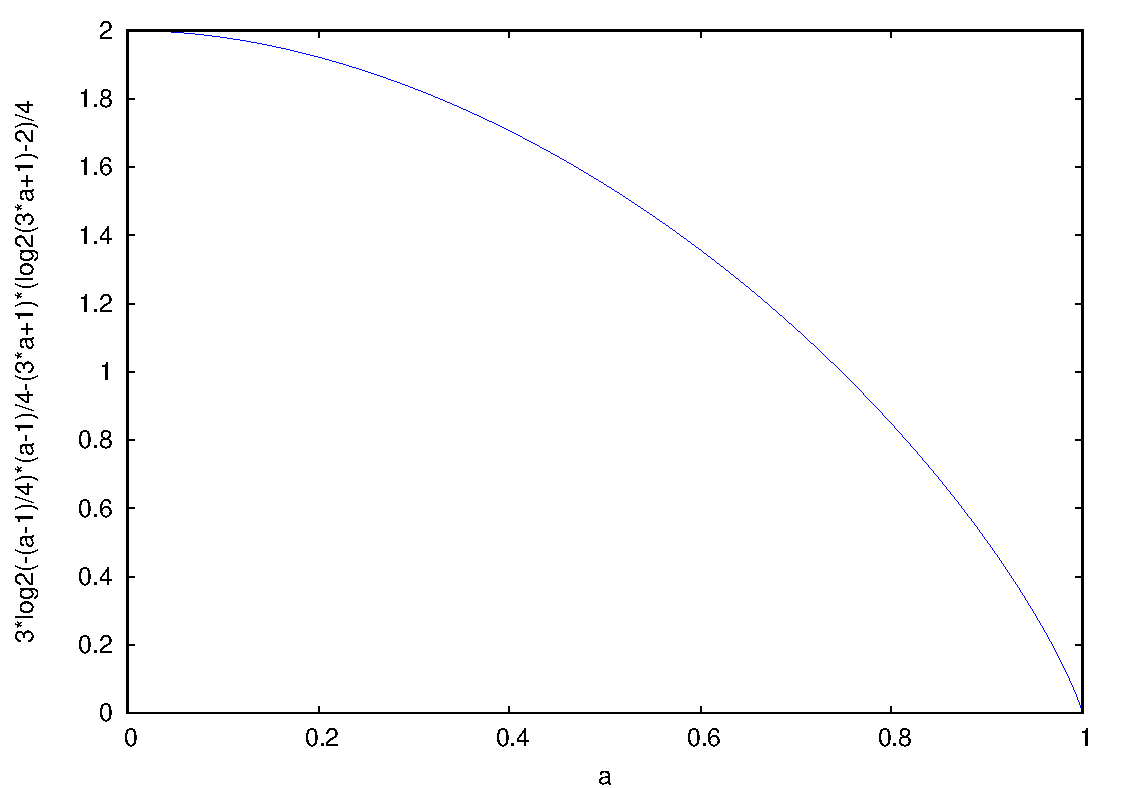
\includegraphics[width=.5\linewidth]{figs/werner_entropy}
\end{dmath}
\ebm

\htmlrule
\section{Creating and using operators}

\subsection{Pauli matrices}\index{pauli matrices}
\subsubsection{\fs{pauli} --- Pauli matrices$.$}
\ibd{pauli}
\marray{pauli}{i}
creates the Pauli matrices $(\sigma_0,\sigma_1,\sigma_2,\sigma_3)
=(\mathbb{1}_2,\sigma_x,\sigma_y,\sigma_z).$
\bbm
\begin{verbatim}
(%i12) [ pauli[0], pauli[1], pauli[2], pauli[3] ];
\end{verbatim}
\begin{dmath}[number={\%o12}]
 \left[ \pmatrix{1&\linebreak[0]0\cr 0&\linebreak[0]1\cr },\linebreak[0]\pmatrix{0&\linebreak[0]1\cr 1&\linebreak[0]0\cr },\linebreak[0]\pmatrix{0&\linebreak[0]-i\cr i&\linebreak[0]0\cr },\linebreak[0]\pmatrix{1&\linebreak[0]0\cr 0&\linebreak[0]-1\cr } \right] \end{dmath}
\ebm
Show that the ket $\ket{1}_x$ is an eigenvector of $\sigma_x$ with eigenvalue $-1$.
\bbm
\begin{verbatim}
(%i8) is (  pauli[1] . ket_n(1,1) = -1 * ket_n(1,1) );
\end{verbatim}
\begin{dmath}[number={\%o8}]
 \mathbf{true}\end{dmath}
\ebm
Here are we check that all our definitions of the Pauli matrices and kets are
consistent in this sense.
\bbm
\begin{verbatim}
(%i9) mapapply( lambda([i,j], is (pauli[i] . ket_n(i,j) = (-1)^j * ket_n(i,j))),
         [[1,0],[1,1],[2,0],[2,1],[3,0],[3,1]  ]);
\end{verbatim}
\begin{dmath}[number={\%o9}]
 \left[ \mathbf{true},\linebreak[0]\mathbf{true},\linebreak[0]\mathbf{true},\linebreak[0]\mathbf{true},\linebreak[0]\mathbf{true},\linebreak[0]\mathbf{true} \right] \end{dmath}
\ebm

Here we use \func{anticommutator}{op_1,op_2} \ibd{anticommutator} to test the anticommutation relations among
the Pauli matrices: $\{\sigma_i,\sigma_j\}= 2\delta_{i,j}$ for $i,j \in\{1,2,3\}.$
\bbm
\ibd{genmatrix}
\begin{verbatim}
(%i3) genmatrix(lambda([i,j],  anticommutator(pauli[i],pauli[j])/2 ), 3,3,1,1);
\end{verbatim}
\begin{dmath}[number={\%o3}]
  \pmatrix{\pmatrix{1&\linebreak[0]0\cr 0&\linebreak[0]1\cr
    }&\linebreak[0]\pmatrix{0&\linebreak[0]0\cr
      0&\linebreak[0]0\cr
    }&\linebreak[0]\pmatrix{0&\linebreak[0]0\cr
      0&\linebreak[0]0\cr }\cr \pmatrix{0&\linebreak[0]0\cr
      0&\linebreak[0]0\cr
    }&\linebreak[0]\pmatrix{1&\linebreak[0]0\cr
      0&\linebreak[0]1\cr
    }&\linebreak[0]\pmatrix{0&\linebreak[0]0\cr
      0&\linebreak[0]0\cr }\cr \pmatrix{0&\linebreak[0]0\cr
      0&\linebreak[0]0\cr
    }&\linebreak[0]\pmatrix{0&\linebreak[0]0\cr
      0&\linebreak[0]0\cr
    }&\linebreak[0]\pmatrix{1&\linebreak[0]0\cr
      0&\linebreak[0]1\cr }\cr }\end{dmath}
\ebm 
The \pname{Maxima} function 
\umaxman{mat\_unblocker}{\maximamatUunblocker}\index{block matrix!flattening block structure},
 flattens the
blocks in the above expression, so we can write \bbm
\begin{verbatim}
(%i4) identitymatrixp( mat_unblocker (genmatrix(lambda([i,j],  
         anticommutator(pauli[i],pauli[j])/2 ), 3,3,1,1)));
\end{verbatim}
\begin{dmath}[number={\%o4}]
  \mathbf{true}\end{dmath} \ebm Now we load the
\umaxman{itensor}{\maximaitensor} package, which provides the \index{levi-civita
  tensor} \umaxman{levi-civita}{\maximaleviUcivita} tensor, and make use of the
\pname{Maxima} functions 
\umaxman{permutations}{\maximapermutations}
(which returns
the \maxman{set}{\maximaSets} of all permutations of a list)
and \umaxman{listify}{\maximalistify} (which converts the set data type into the (ordered) list data type).
The \qinf package provides \ibd{mapapply}
\func{mapapply}{func,[list1, list2,\ldots]}, which
\ifs{apply}s \farg{func} to each of the \farg{list}s and
returns a list of the results.  (see the \pname{Maxima}
documentation for
 \umaxman{apply}{\maximaapply}.)  With all these, we can test
the commutation relations \index{commutator} of the Pauli
matrices. (In reality, the matrix definitions are not
complicated, we are actually testing the other functions.):
$[\sigma_i,\sigma_j] = 2i\epsilon_{i,j,k}\sigma_k$.  \bbm
\begin{verbatim}
(%i5) load("itensor");
\end{verbatim}
\begin{dmath}[number={\%o5}]
 \verb|/usr/share/maxima/5.15.0/share/tensor/itensor.lisp|\end{dmath}
\begin{verbatim}
(%i6) mapapply(lambda([i,j,k],zeromatrixp(commutator(pauli[i],pauli[j]) 
     - 2*%i*levi_civita([i,j,k])*pauli[k])), listify(permutations([1,2,3])));
\end{verbatim}
\begin{dmath}[number={\%o6}]
 \left[ \mathbf{true},\linebreak[0]\mathbf{true},\linebreak[0]\mathbf{true},\linebreak[0]\mathbf{true},\linebreak[0]\mathbf{true},\linebreak[0]\mathbf{true} \right] \end{dmath}
\ebm

\subsubsection{{\bf pauli\_product} ---  tensor product of Pauli matrices$.$}
\ibd{pauli\_product}
\func{pauli\_product}{i_1,\ldots,i_n} returns the tensor product
$\sigma_{i_1} \otimes \cdots \otimes \sigma_{i_n}$, where the indices
$i_j$ are in $\{0,1,2,3\}$. As elsewhere in this document, $\sigma_0$ is
the $2\times 2$ identity matrix.

The next three functions 
\func{pauliexp}{\rho}, \func{invpauliexp}{c}, and \func{correlation\_tensor}{c,i_1,\ldots,i_n}
are related. An example using them follows their definitions.

\subsubsection{\fs{pauliexp} --- expansion of operator in terms of tensor products of Pauli matrices$.$}
\ibd{pauliexp}\index{expansion!in pauli matrices}
\func{pauliexp}{\rho} returns the correlation tensor,
\index{correlation tensor}
 that is, the coefficients in the expansion of the matrix $\rho$
in tensor products of Pauli matrices. Explicitly, \fs{pauliexp}
returns the coefficients $c_{i_1,\ldots,i_n}$ in
\begin{equation}\label{pauliexp}
 \rho = \sum_{i_1,\ldots,i_n=0}^3 c_{i_1,\ldots,i_n} \ \sigma_{i_1} \otimes \cdots \otimes \sigma_{i_n}.
\end{equation}
$\rho$ must be a $2^n\times 2^n$ matrix. The coefficients are returned as a list
of $2^n\times 2^n$ elements. The place of $c_{i_1,\ldots,i_n}$ in the returned list is determined
by taking ${i_1,\ldots,i_n}$ to be the  binary representation of an integer. For convenience,
the coefficient can be retrieved by index with the function \fs{correlation\_tensor}.

\subsubsection{\fs{invpauliexp} --- inverse of expansion in terms of tensor products of Pauli matrices$.$}
\ibd{invpauliexp}\index{expansion!inverse of expansion in Pauli matrices}
\func{invpauliexp}{c} is the inverse of \fs{pauiexp}. Given a list $c$ representing
the correlation tensor (i.e. expansion coefficients),
 \fs{invpauliexp} returns the matrix $\rho$ given by (\ref{pauliexp}).

\subsubsection{\fs{correlation\_tensor} --- retrieve component of correlation tensor by index$.$}
\ibd{correlation\_tensor}
\func{correlation\_tensor}{c,i_1,\ldots,i_n} returns the expansion coefficient for
the term $\sigma_{i_1} \otimes \cdots \otimes \sigma_{i_n}$ in the expansion of
$\rho$, where $c$ is the list of coefficients in the expansion of $\rho$ as given,
for instance, by \fs{pauliexp}.

\subsubsection{Using \fs{pauliexp} and \fs{invpauliexp}; an example$.$}
Here is an example using the three functions defined above.
First we create three generic $2\times2$ (complex) matrices.
\bbm
\begin{verbatim}
(%i2) m1 : matrix([a1,b1],[c1,d1]);
\end{verbatim}
\begin{dmath}[number={\%o2}]
 \pmatrix{\mathrm{a1}&\linebreak[0]\mathrm{b1}\cr \mathrm{c1}&\linebreak[0]\mathrm{d1}\cr }\end{dmath}
\begin{verbatim}
(%i3) m2 : matrix([a2,b2],[c2,d2]) $
(%i4) m3 : matrix([a3,b3],[c3,d3]) $
\end{verbatim}
\ebm
Here is the tensor product of the three matrices. This is {\it not} a generic element in
the three qubit Hilbert space represented by $M(\mathbb{C},8)$. For instance,
the three matrices have $12$ complex parameters while a generic matrix in
the tensor product space  has $64$ complex parameters.
\bbm
\begin{verbatim}
(%i5) mp : m1 otimes m2 otimes  m3 ;
\end{verbatim}
\begin{dmath}[number={\%o5}]
 \pmatrix{\mathrm{a1}\*\mathrm{a2}\*\mathrm{a3}&\linebreak[0]\mathrm{a1}\*\mathrm{a2}\*\mathrm{b3}&\linebreak[0]\mathrm{a1}\*\mathrm{a3}\*\mathrm{b2}&\linebreak[0]\mathrm{a1}\*\mathrm{b2}\*\mathrm{b3}&\linebreak[0]\mathrm{a2}\*\mathrm{a3}\*\mathrm{b1}&\linebreak[0]\mathrm{a2}\*\mathrm{b1}\*\mathrm{b3}&\linebreak[0]\mathrm{a3}\*\mathrm{b1}\*\mathrm{b2}&\linebreak[0]\mathrm{b1}\*\mathrm{b2}\*\mathrm{b3}\cr \mathrm{a1}\*\mathrm{a2}\*\mathrm{c3}&\linebreak[0]\mathrm{a1}\*\mathrm{a2}\*\mathrm{d3}&\linebreak[0]\mathrm{a1}\*\mathrm{b2}\*\mathrm{c3}&\linebreak[0]\mathrm{a1}\*\mathrm{b2}\*\mathrm{d3}&\linebreak[0]\mathrm{a2}\*\mathrm{b1}\*\mathrm{c3}&\linebreak[0]\mathrm{a2}\*\mathrm{b1}\*\mathrm{d3}&\linebreak[0]\mathrm{b1}\*\mathrm{b2}\*\mathrm{c3}&\linebreak[0]\mathrm{b1}\*\mathrm{b2}\*\mathrm{d3}\cr \mathrm{a1}\*\mathrm{a3}\*\mathrm{c2}&\linebreak[0]\mathrm{a1}\*\mathrm{b3}\*\mathrm{c2}&\linebreak[0]\mathrm{a1}\*\mathrm{a3}\*\mathrm{d2}&\linebreak[0]\mathrm{a1}\*\mathrm{b3}\*\mathrm{d2}&\linebreak[0]\mathrm{a3}\*\mathrm{b1}\*\mathrm{c2}&\linebreak[0]\mathrm{b1}\*\mathrm{b3}\*\mathrm{c2}&\linebreak[0]\mathrm{a3}\*\mathrm{b1}\*\mathrm{d2}&\linebreak[0]\mathrm{b1}\*\mathrm{b3}\*\mathrm{d2}\cr \mathrm{a1}\*\mathrm{c2}\*\mathrm{c3}&\linebreak[0]\mathrm{a1}\*\mathrm{c2}\*\mathrm{d3}&\linebreak[0]\mathrm{a1}\*\mathrm{c3}\*\mathrm{d2}&\linebreak[0]\mathrm{a1}\*\mathrm{d2}\*\mathrm{d3}&\linebreak[0]\mathrm{b1}\*\mathrm{c2}\*\mathrm{c3}&\linebreak[0]\mathrm{b1}\*\mathrm{c2}\*\mathrm{d3}&\linebreak[0]\mathrm{b1}\*\mathrm{c3}\*\mathrm{d2}&\linebreak[0]\mathrm{b1}\*\mathrm{d2}\*\mathrm{d3}\cr \mathrm{a2}\*\mathrm{a3}\*\mathrm{c1}&\linebreak[0]\mathrm{a2}\*\mathrm{b3}\*\mathrm{c1}&\linebreak[0]\mathrm{a3}\*\mathrm{b2}\*\mathrm{c1}&\linebreak[0]\mathrm{b2}\*\mathrm{b3}\*\mathrm{c1}&\linebreak[0]\mathrm{a2}\*\mathrm{a3}\*\mathrm{d1}&\linebreak[0]\mathrm{a2}\*\mathrm{b3}\*\mathrm{d1}&\linebreak[0]\mathrm{a3}\*\mathrm{b2}\*\mathrm{d1}&\linebreak[0]\mathrm{b2}\*\mathrm{b3}\*\mathrm{d1}\cr \mathrm{a2}\*\mathrm{c1}\*\mathrm{c3}&\linebreak[0]\mathrm{a2}\*\mathrm{c1}\*\mathrm{d3}&\linebreak[0]\mathrm{b2}\*\mathrm{c1}\*\mathrm{c3}&\linebreak[0]\mathrm{b2}\*\mathrm{c1}\*\mathrm{d3}&\linebreak[0]\mathrm{a2}\*\mathrm{c3}\*\mathrm{d1}&\linebreak[0]\mathrm{a2}\*\mathrm{d1}\*\mathrm{d3}&\linebreak[0]\mathrm{b2}\*\mathrm{c3}\*\mathrm{d1}&\linebreak[0]\mathrm{b2}\*\mathrm{d1}\*\mathrm{d3}\cr \mathrm{a3}\*\mathrm{c1}\*\mathrm{c2}&\linebreak[0]\mathrm{b3}\*\mathrm{c1}\*\mathrm{c2}&\linebreak[0]\mathrm{a3}\*\mathrm{c1}\*\mathrm{d2}&\linebreak[0]\mathrm{b3}\*\mathrm{c1}\*\mathrm{d2}&\linebreak[0]\mathrm{a3}\*\mathrm{c2}\*\mathrm{d1}&\linebreak[0]\mathrm{b3}\*\mathrm{c2}\*\mathrm{d1}&\linebreak[0]\mathrm{a3}\*\mathrm{d1}\*\mathrm{d2}&\linebreak[0]\mathrm{b3}\*\mathrm{d1}\*\mathrm{d2}\cr \mathrm{c1}\*\mathrm{c2}\*\mathrm{c3}&\linebreak[0]\mathrm{c1}\*\mathrm{c2}\*\mathrm{d3}&\linebreak[0]\mathrm{c1}\*\mathrm{c3}\*\mathrm{d2}&\linebreak[0]\mathrm{c1}\*\mathrm{d2}\*\mathrm{d3}&\linebreak[0]\mathrm{c2}\*\mathrm{c3}\*\mathrm{d1}&\linebreak[0]\mathrm{c2}\*\mathrm{d1}\*\mathrm{d3}&\linebreak[0]\mathrm{c3}\*\mathrm{d1}\*\mathrm{d2}&\linebreak[0]\mathrm{d1}\*\mathrm{d2}\*\mathrm{d3}\cr }\end{dmath}
\ebm
We compute the correlation tensor of \verb|mp|
\bbm
\begin{verbatim}
(%i6) pe : pauliexp(mp) $
\end{verbatim}
\ebm
Check that the tensor has $64$ elements and see what a coefficient looks like.
\bbm
\begin{verbatim}
(%i7) length(pe);
\end{verbatim}
\begin{dmath}[number={\%o7}]
 64\end{dmath}
\begin{verbatim}
(%i8) part(pe,10);
\end{verbatim}
\begin{dmath}[number={\%o8}]
 \ifracn{-i\*\mathrm{c1}\*\mathrm{c2}\*\mathrm{d3}-i\*\mathrm{b1}\*\mathrm{c2}\*\mathrm{d3}+i\*\mathrm{b2}\*\mathrm{c1}\*\mathrm{d3}+i\*\mathrm{b1}\*\mathrm{b2}\*\mathrm{d3}-i\*\mathrm{a3}\*\mathrm{c1}\*\mathrm{c2}-i\*\mathrm{a3}\*\mathrm{b1}\*\mathrm{c2}+i\*\mathrm{a3}\*\mathrm{b2}\*\mathrm{c1}+i\*\mathrm{a3}\*\mathrm{b1}\*\mathrm{b2}}{8}\end{dmath}
\ebm
Check that the inverse of the expansion gives the original matrix back
\bbm
\begin{verbatim}
(%i9) is ( ratsimp( invpauliexp( pauliexp(mp) )) = mp);
\end{verbatim}
\begin{dmath}[number={\%o9}]
 \mathbf{true}\end{dmath}
\ebm
Here is the convenience function to return an element of the correlation tensor by index
\bbm
\begin{verbatim}
(%i10) correlation_tensor(pe,1,2,3);
\end{verbatim}
\begin{dmath}[number={\%o10}]
 \ifracn{i\*\mathrm{c1}\*\mathrm{c2}\*\mathrm{d3}+i\*\mathrm{b1}\*\mathrm{c2}\*\mathrm{d3}-i\*\mathrm{b2}\*\mathrm{c1}\*\mathrm{d3}-i\*\mathrm{b1}\*\mathrm{b2}\*\mathrm{d3}-i\*\mathrm{a3}\*\mathrm{c1}\*\mathrm{c2}-i\*\mathrm{a3}\*\mathrm{b1}\*\mathrm{c2}+i\*\mathrm{a3}\*\mathrm{b2}\*\mathrm{c1}+i\*\mathrm{a3}\*\mathrm{b1}\*\mathrm{b2}}{8}\end{dmath}
\ebm

\subsection{\fs{spinor\_rotation}, \fs{spinor\_rotation\_trig}$.$}
\ibd{spinor\_rotation}\ibd{spinor\_rotation\_trig}
\index{rotation!spinor}
\func{spinor\_rotation}{phi,theta,gamma} returns the matrix that represents
the operator that rotates a spinor through an angle \farg{gamma} about the axis specified by 
\farg{phi} (angle about the $z$-axis) and \farg{theta} (inclination from the $z$-axis). The function \func{spinor\_rotation\_trig}{phi,theta,gamma}
returns the same matrix expressed only with cosines and sines. This is the standard
axis-angle parameterization.  Explicitly the matrices are
\bbm
\begin{verbatim}
(%i2) spinor_rotation(phi,theta,gamma);
\end{verbatim}
\begin{dmath}[number={\%o2}]
 \pmatrix{\cos \left(\frac{\gamma}{2}\right)-i\*\cos \vartheta\*\sin \left(\frac{\gamma}{2}\right)&\linebreak[0]-i\*\iexpt{e}{- i\*\varphi }\*\sin \vartheta\*\sin \left(\frac{\gamma}{2}\right)\cr -i\*\iexpt{e}{i\*\varphi}\*\sin \vartheta\*\sin \left(\frac{\gamma}{2}\right)&\linebreak[0]i\*\cos \vartheta\*\sin \left(\frac{\gamma}{2}\right)+\cos \left(\frac{\gamma}{2}\right)\cr }\end{dmath}
\begin{verbatim}
(%i3) spinor_rotation_trig(phi,theta,gamma);
\end{verbatim}
\begin{dmath}[number={\%o3}]
 \pmatrix{\cos \left(\frac{\gamma}{2}\right)-i\*\cos \vartheta\*\sin \left(\frac{\gamma}{2}\right)&\linebreak[0]\left(-\sin \varphi\*\sin \vartheta-i\*\cos \varphi\*\sin \vartheta\right)\*\sin \left(\frac{\gamma}{2}\right)\cr \left(\sin \varphi\*\sin \vartheta-i\*\cos \varphi\*\sin \vartheta\right)\*\sin \left(\frac{\gamma}{2}\right)&\linebreak[0]i\*\cos \vartheta\*\sin \left(\frac{\gamma}{2}\right)+\cos \left(\frac{\gamma}{2}\right)\cr }\end{dmath}.
\ebm

\subsection{\fs{insert\_operator} --- insert single qubit operators in $n$-qubit operator}
 \ibd{insert\_operator}
\func{insert\_operator}{nbits,[op1,i1,i2,..],[op2,j2,j2,...],...} returns
the operator $\mathbb{1}_2^{\otimes \mbox{nbits}}$, with some of the identity operators
$\mathbb{1}_2$ substituted by the operators \farg{op1,op2,\ldots} at the indices specified
by the indices $i1,i2,\ldots,j1,j2,\ldots$. Each replacement operator replaces a single
qubit identity operator $\mathbb{1}_2$, even if the replacement operator has dimension
other than $2$. 
 For example

\begin{center} 
\verb|insert_operator(8,[pauli[1],1,3],[pauli[2],2,5],[pauli[3],8])|
\end{center}
returns
$$
\sigma_x \otimes \sigma_y \otimes \sigma_x \otimes \mathbb{1}_2 
  \otimes \sigma_y \otimes  \mathbb{1}_2 \otimes  \mathbb{1}_2   \otimes \sigma_z.
$$
\fs{insert\_operator} is used to build the operators and gates listed below.

\subsection{Gates}
\index{gates}
\subsubsection{\fs{hadamard} operator$.$}
\ibd{hadamard}
\pname{qinf} defines both a variable and a function named \fs{hadamard}.
The value of the  variable \fs{hadamard} is as follows,
\bbm
\begin{verbatim}
(%i2) hadamard;
\end{verbatim}
\begin{dmath}[number={\%o2}]
 \pmatrix{\ifracd{1}{\isqrt{2}}&\linebreak[0]\ifracd{1}{\isqrt{2}}\cr \ifracd{1}{\isqrt{2}}&\linebreak[0]-\ifracd{1}{\isqrt{2}}\cr }\end{dmath}
\ebm
The function \func{hadamard}{nbits,i1,i2,\ldots}  returns the tensor product
of \farg{nbits} one-qubit operators each of which is $\mathbb{1}_2$ except
for the operators in positions \farg{i1,i2,\ldots} which are the hadamard
operator given by the variable \fs{hadamard}. The function is defined
by
\begin{verbatim}
hadamard(nbits,[t]) := insert_operator(nbits,cons(hadamard,t)),
\end{verbatim}
which is an idiom that will work for similar user defined functions as well.
The dummy argument \verb|[t]| causes all arguments after \verb|nbits| to
be collected in a single list. The \pname{Maxima} function 
\umaxman{cons}{\maximacons}, invoked as \func{cons}{expr,list},
returns the list given by  prepending 
 \verb|expr| to the list \verb|list|. 

\subsubsection{\fs{controlled\_gate} --- gate with $n$ control qubits}
\ibd{controlled\_gate}
A controlled gate applies an operator $m$ to a single qubit (the target) in a register only if
each of a set of control qubits is set. Otherwise the operator is equivalent to
the identity operator. In any case, the operator is the identity on every
qubit other than the target.
The function \func{controlled\_gate}{nbits,qop,t,clst}
creates a controlled gate with one or more control qubits embedded in
a \verb|nbits|-qubit operator. The target qubit is at the index \verb|t|,
while the control qubits are at the indices listed in the list \verb|clst|.
In the returned operator, the $\mathbb{1}_2$ operator is at the remaining positions.
The controlled gate operator applies \verb|qop| at qubit \verb|t| if all of
the control qubits are set (i.e. are $1$) and is equivalent to the identity operator
otherwise.
For instance a \fs{cnot}\index{cnot} operator on $H_2\otimes H_2$ is given by
\verb|controlled_gate(2,pauli[1],2,[1])|.
The controlled gate in an $n$-qubit space with $n-1$ control bits and
the $1$-qubit target operator $m$ is implemented in \pname{qinf} as
$$
 \mathbb{1}_{2^n} + \left(\ket{1}\bra{1}\right)^{\otimes{n-1}}
    \otimes (m-\mathbb{1}_2).
$$
In the case that this  controlled gate operator is embedded in an operator in a larger space,
the same formula is used, with additional factors of $\mathbb{1}_2$ inserted at the 
appropriate places. Also the target qubit may occupy any index. This is implemented
via the \fs{insert\_operator} function described above.

\subsubsection{\fs{cnot}, \fs{cphase}, \fs{crot}$.$}
\ibd{cnot}\ibd{cphase}\ibd{crot}
 \func{cnot}{nbits,t,c1,c2,\ldots} returns a cnot gate on an \verb|nbits|-qubit
register with the target at index \verb|t| and control qubits at indices
\verb|c1,c2,...|. The definition of this function is
\verb|cnot(nbits,t,[c]) := controlled_gate(nbits,pauli[1],t,c)|.
The functions \fs{cphase} and \fs{crot} are defined in the same way except
that operators \verb|pauli[3]| and  \verb|%i*pauli[2]| respectively are
substituted for \verb|pauli[1]|. For example, the elementary cnot gate
is given by \verb|cnot(2,2,1)|.
\subsubsection{\fs{swap}$.$}
\ibd{swap}
\func{swap}{nbits,t1,t2} returns the operator that swaps qubits \verb|t1|
and \verb|t2| in an  \verb|nbits|-qubit register. It is defined by
\verb|swap(nbits,t1,t2) := cnot(nbits,t1,t2) . cnot(nbits,t2,t1) . cnot(nbits,t1,t2)|.
\subsubsection{\fs{toffoli}$.$}
\ibd{toffoli}
This function is provided for convenience. It is defined by
\verb|toffoli(nbits,t,c1,c2) := cnot(nbits,t,c1,c2)|. Note that there
are exactly two control qubits.
\subsubsection{\fs{fredkin}$.$}
\ibd{fredkin}
\func{fredkin}{nbits,t1,t2,c} is controlled swap operator. The qubits at indices
\verb|t1| and \verb|t2| are swapped if the control qubit at index \verb|c| is set.
\htmlrule
%\section{Entanglement-- \func{ptrace}{\rho,i_1,\ldots}, \func{entropy}{\rho}, \func{purity}{\rho}$.$}
\section{Entanglement}

Now we are ready to introduce features that are more
specific to the study quantum entanglement. Included here
are measures of the degree of purity and measures
of the degree of entanglement. For a review of quantum
entanglement, see Ref.\cite{HHH08}.

% namely the partial trace \fs{ptrace}, the von Neumann entropy
%\fs{entropy} and \fs{purity}.


\subsection{\fs{ptrace}, \fs{ptracen} --- partial trace$.$}
\ibd{ptrace}\ibd{ptracen}
\index{trace!partial trace of matrix}
compute the partial trace of the  density 
operator $\rho$ over the component spaces given by the indices.
For \ifunc{ptrace}{\rho,i_1,\ldots} the density matrix $\rho$ is assumed to represent
an operator in
$(H_2)^{\otimes m}$, with $n=2$, that is
a tensor product of qubit spaces. For \ifunc{ptracen}{n,\rho,i_1,\ldots} the component
spaces are all $n$-state qudits.

In this example we create three completely generic $3\times3$ matrices, and check that
$$
\mbox{Tr}_{1,2}\left(m_1\otimes m_2\otimes m_3\right) = \left(\mbox{Tr}(m_1)\mbox{Tr}(m_2)\right) m_3
$$
and that
$$
\mbox{Tr}_{3}\left(m_1\otimes m_2\otimes m_3 \right) = \mbox{Tr}(m_3)(m_1\otimes m_2).
$$
 Notice that we use the \pname{Maxima} function 
\umaxman{ratsimp}{\maximaratsimp} to put both sides of the
equation in the same canonical form.  We also make
use of the
 \umaxman{mat\_trace}{\maximamatUtrace}\index{trace!of matrix}
 function ( so named to avoid conflicting
with the code-execution trace function) and the
\umaxman{matrix}{\maximamatrix} function, which creates a matrix
from a list of rows. \index{matrix!trace} \index{matrix!creating}
\bbm
\begin{verbatim}
(%i1) m1 : matrix([a1,b1,c1],[d1,e1,f1],[g1,h1,i1])$

(%i2) m2 : matrix([a2,b2,c2],[d2,e2,f2],[g2,h2,i2])$

(%i3) m3 : matrix([a3,b3,c3],[d3,e3,f3],[g3,h3,i3])$

(%i4) is ( ratsimp( ptracen(3, m1 otimes m2 otimes m3 , 1,2) = 
            mat_trace(m1)*mat_trace(m2)*m3));
\end{verbatim}
\begin{dmath}[number={\%o4}]
 \mathbf{true}\end{dmath}
\begin{verbatim}
(%i5) is ( ratsimp( ptracen(3, m1 otimes m2 otimes m3 ,3) = mat_trace(m3)* m1 otimes m2));
\end{verbatim}
\begin{dmath}[number={\%o5}]
 \mathbf{true}\end{dmath}
\ebm
Here we trace over one component repeatedly and check that the result is
equal to the full trace. Note that, each time, we are tracing over the new
first component.
\bbm
\begin{verbatim}
(%i10) factor( ptracen(3,ptracen(3,ptracen(3,m1 otimes m2 otimes m3,1),1),1));
\end{verbatim}
\begin{dmath}[number={\%o10}]
 \pmatrix{\left(\mathrm{i1}+\mathrm{e1}+\mathrm{a1}\right)\*\left(\mathrm{i2}+\mathrm{e2}+\mathrm{a2}\right)\*\left(\mathrm{i3}+\mathrm{e3}+\mathrm{a3}\right)\cr }\end{dmath}
\ebm

\subsection{\fs{entropy} --- von Neumann entropy$.$}
\ibd{entropy}
\index{entropy!von Neumann}
\func{entropy}{\rho} returns the von Neumann \fs{entropy} of
the density matrix $\rho$  defined by
\begin{equation}
 S(\rho) = -\mbox{Tr}\left(\rho \log_2 \rho\right).
\end{equation}
\ifs{entropyf} is the floating point version of \fs{entropy}.

\subsection{\fs{renyi\_entropy}$.$}
\ibd{renyi\_entropy}
\index{entropy!R\'enyi}
 \func{renyi\_entropy}{alpha,rho} gives the R\'enyi entropy, defined by
\begin{equation}
 S_{\mbox{renyi}}(\alpha,\rho) = \frac{1}{1-\alpha}\log_2\left(\mbox{Tr}(\rho^\alpha)\right).
\end{equation}
\ifs{renyi\_entropyf} is the floating point version of \fs{renyi\_entropy}.

\subsection{\fs{tsallis\_entropy}$.$}
\ibd{tsallis\_entropy}
\index{entropy!Tsallis}
 \func{tsallis\_entropy}{q,rho} gives the Tsallis entropy, defined by
\begin{equation}
 S_{\mbox{tsallis}}(q,\rho) = \frac{1}{q-1}\left(1-\mbox{Tr}(\rho^q)\right).
\end{equation}
\ifs{tsallis\_entropyf} is the floating point version of \fs{tsallis\_entropy}.

\subsection{\fs{purity}$.$}
\ibd{purity}
 \func{purity}{\rho} returns the purity of the 
density matrix $\rho$ defined by $\mbox{Tr}(\rho^2)$. The purity
is $1$ for a pure state and is less than $1$ for a mixed state.

\subsection{\fs{fidelity}$.$}
\ibd{fidelity}
\func{fidelity}{\rho_1,\rho_2} returns the scalar valued fidelity
of the density matrices $\rho_1$ and $\rho_2$ defined by
$$
 \mbox{Tr}\left(\sqrt{\sqrt{\rho_2}\rho_1\sqrt{\rho_2}}\right).
$$

\subsection{\fs{concurrence} --- Wootters'  concurrence$.$}
\ibd{concurrence}\index{Wootters}
The concurrence of a two-qubit state $\rho$ is defined by 
$\max(0,\sqrt{\lambda_1}-\sqrt{\lambda_2}-\sqrt{\lambda_3}-\sqrt{\lambda_4}$),
where the $\lambda_i$ are the eigenvaluse of
$$
  \rho (\sigma_y \otimes \sigma_y) \rho^{\mbox{*}} (\sigma_y \otimes \sigma_y),
$$
in decreasing order\cite{Wootters97}

\verb|concurrence(rho)| returns the concurrence of the state \verb|rho|.
\verb|concurrence_vals(rho)| returns a list of the square roots of
the eigenvalues in decreasing order, to the extent that \pname{Maxima}
can determine the order.

\subsection{\fs{separable} --- test for separability$.$}\index{separability}
\ibd{separable}
This currently accepts only pure, bipartite states.
\func{separable}{e} attempts to determine if \farg{e} is a separable
state. \fs{separable} returns a scalar value $r$. If $r=1$, then
\farg{e} is separable. If $r<1$, it is not. Explicitly, the value
returned for the state with density operator $\rho_{AB}$ 
is $\mbox{Tr}(\rho_A^2)$

\subsection{Example: An entangled pure global state has mixed reduced states}
We examine a textbook example of entanglement--- the
pure join state of two qubits. The state of the whole system is pure,
but the local states are mixed.  We begin by creating a
joint state of two qubits in Schmidt basis
$\ket{\alpha}=\sqrt{\alpha}\ket{00}+
\sqrt{1-\alpha}\ket{11}.$ In order to see the mixed
character of the local states, we need to express the full
state as a density operator (or equivalently as a projection
operator.) Let's try to make $\ket{\alpha}\bra{\alpha}$.
\bbm
\begin{verbatim}
(%i2)  pr : proj(schmidt_ket(alpha));
\end{verbatim}
\begin{dmath}[number={\%o2}]
 \pmatrix{\isqrt{\alpha}^{\star}\*\isqrt{\alpha}&\linebreak[0]0&\linebreak[0]0&\linebreak[0]\isqrt{1-\alpha}^{\star}\*\isqrt{\alpha}\cr 0&\linebreak[0]0&\linebreak[0]0&\linebreak[0]0\cr 0&\linebreak[0]0&\linebreak[0]0&\linebreak[0]0\cr \isqrt{\alpha}^{\star}\*\isqrt{1-\alpha}&\linebreak[0]0&\linebreak[0]0&\linebreak[0]\isqrt{1-\alpha}^{\star}\*\isqrt{1-\alpha}\cr }
\end{dmath}
\ebm
We see that \pname{Maxima} is allowing that the quantities under the radicals may be negative. So
we set some rules, and try again. \ibd{assume}
\bbm
\begin{verbatim}
(%i3) assume(alpha>0, 1-alpha>0);
\end{verbatim}
\begin{dmath}[number={\%o4}]
 \left[ \alpha>0,\linebreak[0]\alpha<1 \right] \end{dmath}
\begin{verbatim}
(%i5)  pr : proj(schmidt_ket(alpha));
\end{verbatim}
\begin{dmath}[number={\%o5}]
 \pmatrix{\alpha&\linebreak[0]0&\linebreak[0]0&\linebreak[0]\isqrt{1-\alpha}\*\isqrt{\alpha}\cr 0&\linebreak[0]0&\linebreak[0]0&\linebreak[0]0\cr 0&\linebreak[0]0&\linebreak[0]0&\linebreak[0]0\cr \isqrt{1-\alpha}\*\isqrt{\alpha}&\linebreak[0]0&\linebreak[0]0&\linebreak[0]1-\alpha\cr }\end{dmath}
\ebm
The entropy \index{entropy!of a pure state}
 vanishes for a pure state, so that $S(\ket{\alpha}\bra{\alpha})$ is
\bbm
\begin{verbatim}
(%i6)  entropy(pr);
\end{verbatim}
\begin{dmath}[number={\%o7}]
 0\end{dmath}
\ebm
The \ifs{purity} is equal to $1$ if and only if $\rho$ is a pure state.
\bbm
\begin{verbatim}
(%i8) purity(pr);
\end{verbatim}
\begin{dmath}[number={\%o8}]
 \alpha^{2}+2\*\left(1-\alpha\right)\*\alpha+\left(1-\alpha\right)^{2}\end{dmath}
The above line should be 
\maxman{simplified}{maxima_7.html#SEC29} by writing it as a canonical rational expression (CRE)
\ibd{ratsimp} \index{canonical rational expression}
\begin{verbatim}
(%i9) ratsimp(%);
\end{verbatim}
\begin{dmath}[number={\%o9}]
 1\end{dmath}
\ebm
Now we compute the reduced density matrix of the second qubit by tracing over the first---
$\rho_2=\mbox{Tr}_1 \ket{\alpha}\bra{\alpha}.$
\bbm
\begin{verbatim}
(%i10)  pr2 : ptrace(pr,1);
\end{verbatim}
\begin{dmath}[number={\%o10}]
 \pmatrix{\alpha&\linebreak[0]0\cr 0&\linebreak[0]1-\alpha\cr }\end{dmath}
\ebm
Tracing over the second qubit instead gives the same result
\bbm
\begin{verbatim}
(%i11) ptrace(pr,2);
\end{verbatim}
\begin{dmath}[number={\%o11}]
  \pmatrix{\alpha&\linebreak[0]0\cr
    0&\linebreak[0]1-\alpha\cr }\end{dmath} \ebm Computing
the entropy\index{entropy!of a reduced state} of a local state
shows that this state is, in general, mixed \bbm
\ibd{entropy}
\begin{verbatim}
(%i12) entropy(pr2);
\end{verbatim}
\begin{dmath}[number={\%o12}]
 -\alpha\*\mathrm{log2}\left(\alpha\right)-\mathrm{log2}\left(1-\alpha\right)\*\left(1-\alpha\right)\end{dmath}
\ebm
Each eigenvalue $\lambda$ satisfies $0\le \lambda <1$, so that the sum of their squares is less than
one 
\bbm
\begin{verbatim}
(%i13) purity(pr2);
\end{verbatim}
\begin{dmath}[number={\%o13}]
  \alpha^{2}+\left(1-\alpha\right)^{2}\end{dmath} \ebm We
can plot \index{plotting} the results (the plot function \ifs{plot2d} is more
common, depending on your user interface. \ifs{wxplot2d} has
the same calling syntax, but inlines the resulting plot.) We
see that the maximum entanglement occurs at $\alpha=1/2$ and
decreases monotonically from there in both directions, with
$\alpha=0,1$ giving pure joint states.  \bbm
\begin{verbatim}
(%i14)  wxplot2d([entropy(pr2), purity(pr2)],[alpha,0,1]);
\end{verbatim}
\begin{dmath}[number={\%o14}]
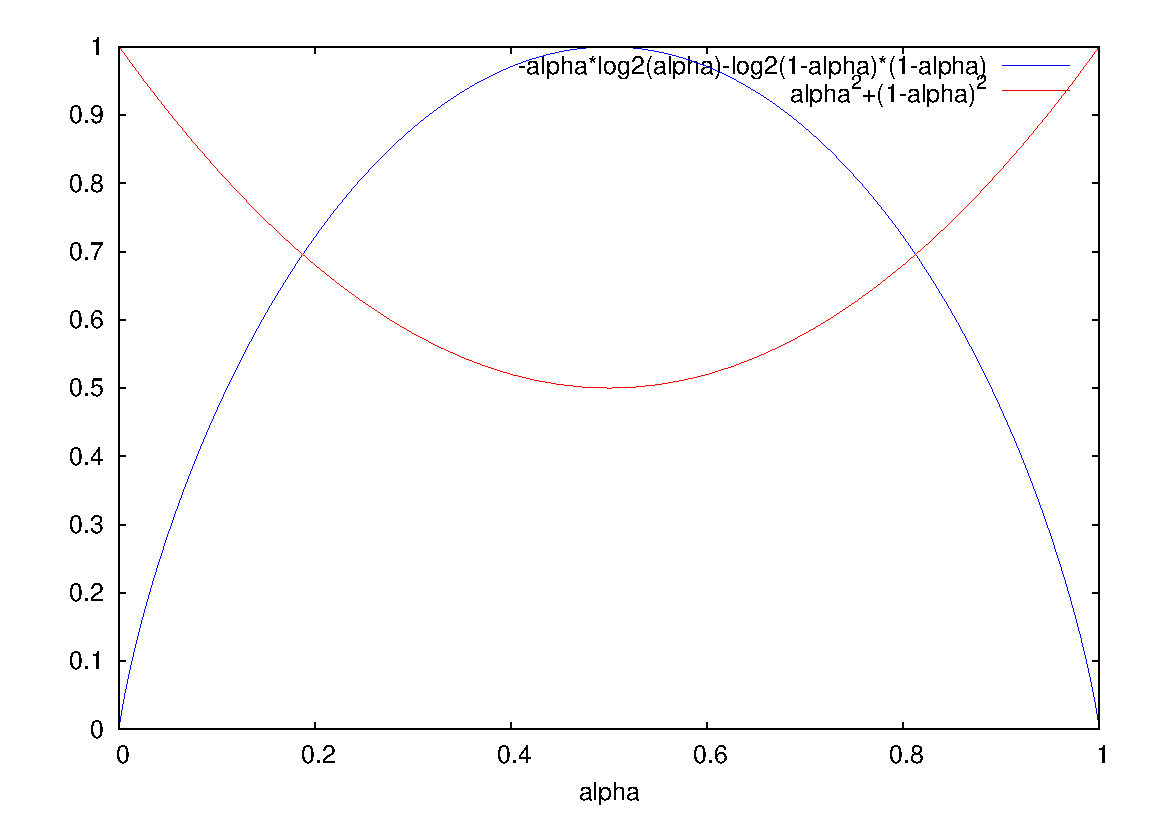
\includegraphics[width=.5\linewidth]{figs/entropy_purity}
\end{dmath}
\ebm

\htmlrule
\section{More operators and functions}

Unless noted, all functions return either true or false.

\subsection{Predicate functions --- testing for properties}
\subsubsection{\fs{identitymatrixp} }\ibd{identitymatrixp}
 \index{identity matrix!testing for}
\func{identitymatrixp}{e} returns  true if \farg{e} is the $n\times n$ identity
 matrix for any $n$.
\subsubsection{\fs{ketp}, \fs{brap}, \fs{braketp}}\ibd{ketp}\ibd{brap}\ibd{braketp}
\func{ketp}{e} returns true if the expression \farg{e} is a ket
(column vector).
\func{brap}{e} returns true if the expression \farg{e} is a bra
(row vector).
 \func{braketp}{e}
returns \verb|(ketp(e) or brap(e))|, i.e. returns true if \farg{e} is either a ket or
a bra.
\subsubsection{\fs{square\_matp}}\ibd{square\_matp}
\func{square\_matp}{e} returns true if \farg{e} is a square matrix.
\subsection{Miscellaneous}
\subsubsection{\fs{normalize\_vector}}\ibd{normalize\_vector}
  \func{normalize\_vector}{v} returns $v/\bracket{v}{v}$.
\subsubsection{\fs{normalize\_operator}}\ibd{normalize\_matrix}
  \func{normalize\_matrix}{m} returns $m/\mbox{Tr}(m)$.

\htmlrule
\section{Reproducible research}

\subsection{Entanglement swapping\index{entanglement swapping}}

In this subsection, we check a calculation 
(appearing in Ref.~\cite{perseguers:022308})
that would
be relatively difficult to check by hand.
Consider a pair of entangled qubits $A$ and $B$, and another
entangled pair $C$ and $D$. By performing a joint
measurement on, say $B$ and $C$, we can put $A$ and $B$ in
an entangled state although they may be widely separated.
We begin by considering the most general projective measure
on $B$ and $C$, and calculate the reduced density matrix for
a single qubit and the probability of outcome. In this
example we calculate these quantities two ways--- one,
directly from the density matrix formalism, and two, via
formulas taking advantage of the particulars of this
problem. To do the first calculation by hand would be
extremely unpleasant, as it involves multiplying $16\times16$
matrices with several factors in a single element. Carrying
it out below with \pname{Maxima} is a concise exercise.

Qubits $A$ and $B$ are in the state
$$
\ket{\alpha}=\sqrt{\alpha}\ket{00}+ \sqrt{1-\alpha}\ket{11},
$$
$C$ and $D$ are in the state
$$
\ket{\beta}=\sqrt{\beta}\ket{00}+ \sqrt{1-\beta}\ket{11},
$$
with the Schmidt coefficients \index{Schmidt coefficients}
satisfying $\alpha,\beta >1/2$.
For now, we only want to tell \pname{Maxima} that the coefficients
of the kets are real.\ibd{assume}
 \bbm
\begin{verbatim}
(%i2) assume(alpha>0,1-alpha>0,beta>0,1-beta>0);
\end{verbatim}
\begin{dmath}[number={\%o2}]
 \left[ \alpha>0,\linebreak[0]\alpha<1,\linebreak[0]\beta>0,\linebreak[0]\beta<1 \right] \end{dmath}
\begin{verbatim}
(%i3) a : schmidt_ket(alpha);
\end{verbatim}
\begin{dmath}[number={\%o3}]
 \pmatrix{\isqrt{\alpha}\cr 0\cr 0\cr \isqrt{1-\alpha}\cr }\end{dmath}
\begin{verbatim}
(%i4) b : schmidt_ket(beta);
\end{verbatim}
\begin{dmath}[number={\%o4}]
 \pmatrix{\isqrt{\beta}\cr 0\cr 0\cr \isqrt{1-\beta}\cr }\end{dmath}
\ebm
We consider the projective measurement\index{projective measure} $\{E_m\}$, that is $E_m=\ket{u_m}\bra{u_m}$
and $\sum_m E_m=\mathbb{1}_4$. We consider only a single basis vector
here, so we don't use the subscript $m$ for \pname{Maxima} vector name.
We need to use the
\umaxman{declare}{\maximadeclare} function to declare that 
the components are complex. \index{complex numbers!declaring variable complex}
The state $\ket{u_m}$ is normalized, but we don't need to impose that condition in
\pname{Maxima} at this point.
\bbm
\begin{verbatim}
(%i5)  declare([u00,u01,u10,u11], complex);
\end{verbatim}
\begin{dmath}[number={\%o5}]
 \mathbf{done}\end{dmath}
\begin{verbatim}
(%i6) u : ket(u00,u01,u10,u11);
\end{verbatim}
\begin{dmath}[number={\%o6}]
 \pmatrix{\mathrm{u00}\cr \mathrm{u01}\cr \mathrm{u10}\cr \mathrm{u11}\cr }\end{dmath}
\ebm
The initial joint state $\ket{\alpha\beta}\bra{\alpha\beta}$ is pure and remains
so after the measurement applying $\ket{u_m}\bra{u_m}$ to qubits $B$ and $C$.
But we write the density operator
because we will examine the reduced states, which are mixed.
In the case that $B$ and $C$ are projected onto $\ket{u_m}$, the state
of the entire system of four qubits after the measurement is given by
\begin{equation}
  \rho = \left( (\mathbb{1}_2 \otimes \ket{u_m}\bra{u_m} \otimes \mathbb{1}_2 )
     \ket{\alpha\beta}\bra{\alpha\beta}\right),   
\end{equation}
with
\bbm
\begin{verbatim}
(%i7) rho : conjsimp((ident(2) otimes proj(u) otimes ident(2)) . proj(a otimes b))$,
\end{verbatim}
\ebm
where \ifs{conjsimp} 
(supplied via the \pname{Maxima} listserv by Barton Willis) replaces $xx^*$ with $|x|^2$,
and $\ifunc{ident}{n}$ \index{identity matrix!creating} is the $n\times n$ identity matrix.
The output was suppressed with the trailing dollar sign because the $\rho$ is
a $16\times16$ matrix with large expressions for entries.
%\everymath{\scriptscriptstyle}
%\newcommand{\myrm}[1]{\scriptscriptstyle{#1}}
%\newcommand{\mylineb}{\scriptscriptstyle \linebreak[0] \scriptscriptstyle }
%\newcommand{\myalpha}{\scriptscriptstyle \alpha }
%\newcommand{\myisqrt}[1]{\scriptscriptstyle\sqrt{#1}}
The reduced state of qubits $A$ and $D$ is obtained by tracing out components $2$ and
$3$ corresponding to qubits $B$ and $C$, i.e. $\rho_{AD} =\mbox{Tr}_{BC}\rho$.
\ibd{ptrace}
\bbm
\begin{verbatim}
(%i8) rho_14 : ptrace(rho,2,3);
\end{verbatim}
\begin{dmath}[number={\%o8},style={\tiny}]
 \pmatrix{\alpha\*\beta\*\left| \mathrm{u00}\right| ^{2}&\linebreak[0]\alpha\*\isqrt{1-\beta}\*\isqrt{\beta}\*\mathrm{u00}^{\star}\*\mathrm{u01}&\linebreak[0]\isqrt{1-\alpha}\*\isqrt{\alpha}\*\beta\*\mathrm{u00}^{\star}\*\mathrm{u10}&\linebreak[0]\isqrt{1-\alpha}\*\isqrt{\alpha}\*\isqrt{1-\beta}\*\isqrt{\beta}\*\mathrm{u00}^{\star}\*\mathrm{u11}\cr \alpha\*\isqrt{1-\beta}\*\isqrt{\beta}\*\mathrm{u00}\*\mathrm{u01}^{\star}&\linebreak[0]\left(\alpha-\alpha\*\beta\right)\*\left| \mathrm{u01}\right| ^{2}&\linebreak[0]\isqrt{1-\alpha}\*\isqrt{\alpha}\*\isqrt{1-\beta}\*\isqrt{\beta}\*\mathrm{u01}^{\star}\*\mathrm{u10}&\linebreak[0]\left(\isqrt{1-\alpha}\*\isqrt{\alpha}-\isqrt{1-\alpha}\*\isqrt{\alpha}\*\beta\right)\*\mathrm{u01}^{\star}\*\mathrm{u11}\cr \isqrt{1-\alpha}\*\isqrt{\alpha}\*\beta\*\mathrm{u00}\*\mathrm{u10}^{\star}&\linebreak[0]\isqrt{1-\alpha}\*\isqrt{\alpha}\*\isqrt{1-\beta}\*\isqrt{\beta}\*\mathrm{u01}\*\mathrm{u10}^{\star}&\linebreak[0]\left(1-\alpha\right)\*\beta\*\left| \mathrm{u10}\right| ^{2}&\linebreak[0]\left(1-\alpha\right)\*\isqrt{1-\beta}\*\isqrt{\beta}\*\mathrm{u10}^{\star}\*\mathrm{u11}\cr \isqrt{1-\alpha}\*\isqrt{\alpha}\*\isqrt{1-\beta}\*\isqrt{\beta}\*\mathrm{u00}\*\mathrm{u11}^{\star}&\linebreak[0]\left(\isqrt{1-\alpha}\*\isqrt{\alpha}-\isqrt{1-\alpha}\*\isqrt{\alpha}\*\beta\right)\*\mathrm{u01}\*\mathrm{u11}^{\star}&\linebreak[0]\left(1-\alpha\right)\*\isqrt{1-\beta}\*\isqrt{\beta}\*\mathrm{u10}\*\mathrm{u11}^{\star}&\linebreak[0]\left(\left(\alpha-1\right)\*\beta-\alpha+1\right)\*\left| \mathrm{u11}\right| ^{2}\cr }\end{dmath}
\ebm
Likewise, the reduced state of just qubit $D$ is
$\rho_{D} =\mbox{Tr}_{ABC}\rho$.\ibd{ptrace}\index{reduced state}
\bbm
\begin{verbatim}
(%i9) rho_4 : ptrace(rho,1,2,3);
\end{verbatim}
\begin{dmath}[number={\%o9}]
 \pmatrix{\left(1-\alpha\right)\*\beta\*\left| \mathrm{u10}\right| ^{2}+\alpha\*\beta\*\left| \mathrm{u00}\right| ^{2}&\linebreak[0]\left(1-\alpha\right)\*\isqrt{1-\beta}\*\isqrt{\beta}\*\mathrm{u10}^{\star}\*\mathrm{u11}+\alpha\*\isqrt{1-\beta}\*\isqrt{\beta}\*\mathrm{u00}^{\star}\*\mathrm{u01}\cr \left(1-\alpha\right)\*\isqrt{1-\beta}\*\isqrt{\beta}\*\mathrm{u10}\*\mathrm{u11}^{\star}+\alpha\*\isqrt{1-\beta}\*\isqrt{\beta}\*\mathrm{u00}\*\mathrm{u01}^{\star}&\linebreak[0]\left(\left(\alpha-1\right)\*\beta-\alpha+1\right)\*\left| \mathrm{u11}\right| ^{2}+\left(\alpha-\alpha\*\beta\right)\*\left| \mathrm{u01}\right| ^{2}\cr }\end{dmath}
\ebm
The second method of calculating $\rho_{D}$ is as follows.
Considering the following map from
$\mathbb{C}^2\otimes\mathbb{C}^2$ to $M(\mathbb{C},2)$:
\begin{equation}\label{ket_to_mat}
    \ket{a}=\sum_{i,j=0}^1 a_{ij}\ket{ij}\quad\mapsto\quad\widehat{a}=
    \pmatrix{
      a_{00} & a_{01} \cr
      a_{10} & a_{11} \cr
    },
\end{equation}
one can show that $\rho_{D}$ is equal to $X_m^{\dagger}X_m$, with
$X_m = \widehat{\alpha}\,\widehat{u}_m\,\widehat{\beta}$.
The \pname{Maxima} function implementing the mapping (\ref{ket_to_mat}) is
\bbm
\begin{verbatim}
(%i10) ket_to_mat(iket) := matrix([iket[1,1],iket[2,1]],[iket[3,1],iket[4,1]])$
\end{verbatim}
\ebm
Then the second calculation of $\rho_D$, which we call \verb|rho_4a| is given by
the following lines.
\bbm
\begin{verbatim}
(%i11) mu : ket_to_mat(u)$
(%i12) X :  ket_to_mat(a) . mu . ket_to_mat(b);
\end{verbatim}
\begin{dmath}[number={\%o12}]
 \pmatrix{\isqrt{\alpha}\*\isqrt{\beta}\*\mathrm{u00}&\linebreak[0]\isqrt{\alpha}\*\isqrt{1-\beta}\*\mathrm{u01}\cr \isqrt{1-\alpha}\*\isqrt{\beta}\*\mathrm{u10}&\linebreak[0]\isqrt{1-\alpha}\*\isqrt{1-\beta}\*\mathrm{u11}\cr }\end{dmath}
\begin{verbatim}
(%i13) rho_4a : conjsimp( ctranspose(X) . X );
\end{verbatim}
\begin{dmath}[number={\%o13}]
 \pmatrix{\left(1-\alpha\right)\*\beta\*\left| \mathrm{u10}\right| ^{2}+\alpha\*\beta\*\left| \mathrm{u00}\right| ^{2}&\linebreak[0]\left(1-\alpha\right)\*\isqrt{1-\beta}\*\isqrt{\beta}\*\mathrm{u10}^{\star}\*\mathrm{u11}+\alpha\*\isqrt{1-\beta}\*\isqrt{\beta}\*\mathrm{u00}^{\star}\*\mathrm{u01}\cr \left(1-\alpha\right)\*\isqrt{1-\beta}\*\isqrt{\beta}\*\mathrm{u10}\*\mathrm{u11}^{\star}+\alpha\*\isqrt{1-\beta}\*\isqrt{\beta}\*\mathrm{u00}\*\mathrm{u01}^{\star}&\linebreak[0]\left(\left(\alpha-1\right)\*\beta-\alpha+1\right)\*\left| \mathrm{u11}\right| ^{2}+\left(\alpha-\alpha\*\beta\right)\*\left| \mathrm{u01}\right| ^{2}\cr }\end{dmath}
\ebm
We compare \verb|(%o9)| and  \verb|(%o13)|, to see that the two methods of calculating
the reduced state for qubit $D$ after the measurement give the same result
\bbm
\begin{verbatim}
(%i14) is ( ratsimp(rho_4a) = ratsimp(rho_4) );
\end{verbatim}
\begin{dmath}[number={\%o14}]
 \mathbf{true}\end{dmath}
\ebm
Now we compute the probability 
$p_m=\mbox{Tr}(\rho)=\mbox{Tr}(\rho_D)$
that the state is in fact projected onto $\ket{u_m}$.
\bbm
\begin{verbatim}
(%i15) P1 : conjsimp( mat_trace(rho));
\end{verbatim}
\begin{dmath}[number={\%o15}]
 \left(\left(\alpha-1\right)\*\beta-\alpha+1\right)\*\left| \mathrm{u11}\right| ^{2}+\left(1-\alpha\right)\*\beta\*\left| \mathrm{u10}\right| ^{2}+\left(\alpha-\alpha\*\beta\right)\*\left| \mathrm{u01}\right| ^{2}+\alpha\*\beta\*\left| \mathrm{u00}\right| ^{2}\end{dmath}
\ebm
Finally, we compare this to the trace computed by hand from the expression following (\ref{ket_to_mat}),
which is given by
\begin{equation}
 p_m=\sum^1_{i,j=0} {\alpha}_{i} {\beta}_{j} |\widehat{u}_{m,ij}|^2,
\end{equation}
where $\alpha_0=\alpha,\  \alpha_1=1-\alpha, \  \beta_0=\beta, \ \beta_1=1-\beta$,
\bbm
\begin{verbatim}
(%i16) av : [alpha,1-alpha]$
(%i17) bv : [beta,1-beta] $
(%i18) P2 : apply( "+", create_list( av[i] * abs(mu[i,j])^2 * bv[j], i,[1,2],j,[1,2]));
\end{verbatim}
\begin{dmath}[number={\%o18}]
 \left(1-\alpha\right)\*\left(1-\beta\right)\*\left| \mathrm{u11}\right| ^{2}+\left(1-\alpha\right)\*\beta\*\left| \mathrm{u10}\right| ^{2}+\alpha\*\left(1-\beta\right)\*\left| \mathrm{u01}\right| ^{2}+\alpha\*\beta\*\left| \mathrm{u00}\right| ^{2}\end{dmath}.
\ebm
Here we have used the
 \umaxman{apply}{\maximaapply} and 
\umaxman{create\_list}{\maximacreateUlist} functions.
Once again we compare the probabilities computed via the two methods
\bbm
\begin{verbatim}
(%i19) is (ratsimp(P1) = ratsimp(P2));
\end{verbatim}
\begin{dmath}[number={\%o19}]
 \mathbf{true}\end{dmath}
\ebm
and see that they give the same result.

Ref.~\cite{perseguers:022308} continues with a
discussion of the measurements that maximize the resulting entanglement
of $A$ and $D$. We have not yet verified this with \pname{qinf}.

\bibliography{qperc}

\htmlrule
\newpage
%\section*{Index}
\addcontentsline{toc}{section}{Index}
\printindex
\htmlrule

%\addcontentsline{toc}{section}{Index}

\end{document}

%  LocalWords:  Lapeyre Chuang Preskill Mermin subexpressions html th
%  LocalWords:  imaxima emacs frontends wxmaxima texmacs qubits qinf
%  LocalWords:  qdensity Dodier Stavros Macrakis Fateman Kets kets
%  LocalWords:  hermitian ctranspose dyad otimes tensorproduct ketz
%  LocalWords:  kronecker braz ketx brax kety multipartite eigenstate
%  LocalWords:  ket partite eigenstates proj expr tovect elementwise
%  LocalWords:  schmidt sqrt belln orthonormality genmatrix ghz ghzn
%  LocalWords:  identitymatrixp zeromatrixp orthonormal gzh gzhn
%  LocalWords:  werner Werner
